\documentclass[11pt]{article}
\usepackage{graphicx}
\usepackage{fullpage}
\usepackage{titlesec}
\usepackage{amsmath}
\usepackage{amsthm}
\usepackage{color}
\usepackage{setspace}
\usepackage{courier}
\usepackage[toc, page]{appendix}
\usepackage{listings}
\usepackage{lmodern}
\usepackage{adjustbox}
\usepackage{amssymb}

\newtheorem{statement}{Statement}

\newcommand{\statenumstate}{8,013-state }
\newcommand{\statenum}{8,013 }
\newcommand{\statenumcomma}{8,013, }
\newcommand{\bbstatenum}{$BB($8,013) }
\newcommand{\bbstatenumcomma}{$BB($8,013), }
\newcommand{\bbstatenumperiod}{$BB($8,013). }

\newcommand{\zhaltstate}{\texttt{7593}}
\newcommand{\ghaltstate}{\texttt{5135}}
\newcommand{\rhaltstate}{\texttt{5137}}

\newcommand{\gbstatenum}{4,888 }
\newcommand{\gbstatenumstate}{4,888-state }
\newcommand{\bbgbstatenum}{$BB($4,888) }

\newcommand{\rmstatenum}{5,372 }
\newcommand{\rmstatenumstate}{5,372-state }
\newcommand{\bbrmstatenum}{$BB($5,372) }

\newenvironment{nscenter}
 {\parskip=0pt\par\nopagebreak\centering}
 {\par\noindent\ignorespacesafterend}

\setcounter{secnumdepth}{4}

\begin{document}

\title{A Relatively Small Turing Machine Whose Behavior Is Independent of Set Theory}
\author{
    Adam Yedidia\\
    \small\texttt{MIT}\\
    \small\texttt{adamy@mit.edu}
    \and
    Scott Aaronson\\
    \small\texttt{MIT}\\
    \small\texttt{aaronson@csail.mit.edu}
}
\maketitle

\begin{abstract}

Since the definition of the Busy Beaver function by Rad\'{o} in 1962, an interesting open question has been what the smallest value of $n$ for which $BB(n)$ is independent of ZFC set theory. Is this $n$ approximately 10, or closer to 1,000,000, or is it even larger? In this paper, we show that it is at most \statenum by presenting an explicit description of a \statenumstate Turing machine $Z$ with 1 tape and a 2-symbol alphabet that cannot be proved to run forever in ZFC (even though it presumably does), assuming ZFC is consistent. The machine is based on work of Harvey Friedman on independent statements involving order-invariant graphs. In doing so, we give the first known upper bound on the highest provable Busy Beaver number in ZFC. We also present an explicit description of a \gbstatenumstate Turing machine $G$ that halts if and only if there is a counterexample to Goldbach's conjecture, and an explicit description of a \rmstatenumstate Turing machine $R$ that halts if and only if the Riemann hypothesis is false. To create $G$, $R$, and $Z$, we develop and use a higher-level language, Laconic, which is much more convenient than direct state manipulation. 

\end{abstract}

\section{Introduction}

%\subsection{Contributions}

%This paper is devoted to demonstrating the extreme difficulty of finding the values of the Busy Beaver function beyond a certain point. We cannot ever prove an upper bound on $BB(x)$ for any $x \ge \gbstatenum$ or $x \ge \rmstatenum$ without simultaneously providing a proof (or disproof) of the Goldbach or Riemann hypotheses, respectively. And we cannot ever prove an upper bound on $BB(x)$ for any $x \ge \statenum$ without assuming axioms more powerful than those of Zermelo-Fraenkel Set Theory with the Axiom of Choice (a.k.a. ZFC), assuming ZFC is consistent.\footnotemark  
%\footnotetext{While we will talk about ZFC throughout this paper, rather than simple Zermelo-Fraenkel set theory, this is simply convention brought about by the fact that ZFC is a more powerful and more commonly-used set of axioms. In fact, for the purposes of this paper, the Axiom of Choice is irrelevant: the consistency of ZFC is equivalent to the consistency of simple ZF set theory,~\cite{godelcohen} and ZFC and ZF prove exactly the same arithmetical statements (which include, among other things, Turing machine execution histories).~\cite{schoenfield}}

%We demonstrate these results by presenting explicit descriptions of Turing machines, $G$, $R$, and $Z$ whose \emph{behavior} (whether or not they halt) implies the truth or falsehood of the Goldbach and Riemann hypotheses and the consistency of ZFC, respectively. If one knew a proof that $\bbstatenum < u_G$ for some $u_G$, one could find out if $G$ halts or loops by running $G$ for $u_G$ steps and seeing if it had halted by then; if it had not, we would be certain that $G$ will never halt. Thus, an execution history of $G$ for $u_G$ steps would constitute a proof of the truth or falsehood of Goldbach's conjecture. The same logic holds for $R$, \bbrmstatenum, and the Riemann hypothesis. 

%Likewise, if one knew a proof that \bbstatenum$ \le u_Z$, one could find out if $Z$ halts or loops by running $Z$ for $u_Z$ steps $Z$ for $u_Z$ steps and seeing if it had halted by then; if it had not, we would be certain that $Z$ will never halt. Thus, an execution history of $Z$ for $u_Z$ steps would constitute a proof in ZFC (since ZFC can encode arithmetic, and therefore Turing machine execution histories) of the consistency or inconsistency of ZFC. By G\"{o}del's second incompleteness theorem, such a proof cannot exist if ZFC is consistent. Thus, no proof in ZFC exists of an upper bound on the value of \bbstatenum, assuming ZFC is consistent.

\subsection{Background and Motivation \label{sec:background}}

\emph{Zermelo-Fraenkel set theory with the axiom of choice}, more commonly known as ZFC, is an axiomatic system invented in the twentieth which has since been used as the foundation of most of modern mathematics. It encodes arithmetic by describing natural numbers as increasing sets of sets. 

Like any axiomatic system capable of encoding arithmetic, ZFC is constrained by G\"{o}del's two incompleteness theorems. The first incompleteness theorem states that if ZFC is \emph{consistent} (it never proves both a statement and its opposite), then ZFC cannot also be \emph{complete} (able to prove every true statement). The second incompleteness theorem states that if ZFC is consistent, then ZFC cannot prove its own consistency. Because we have built modern mathematics on top of ZFC, we can reasonably be said to have assumed ZFC's consistency. This means that we must also believe that ZFC cannot prove its own consistency. This fact carries with it certain surprising conclusions. 

In particular, consider a Turing machine $Z$ that enumerates, one after the other, each of the provable statements in ZFC. To describe how such a machine might be constructed, $Z$ could iterate over the axioms and inference rules of ZFC, applying each in every possible way to each conclusion or pair of conclusions that had been reached so far. We might ask $Z$ to halt if it ever reaches a contradiction; in other words, $Z$ will halt if and only if it ever finds a proof of $0 = 1$. Because we know that this machine will enumerate \emph{every} provable statement in ZFC, we know that it will run forever if and only if ZFC is consistent. 

It follows that $Z$ is a Turing machine for which the question of its behavior (whether or not it halts when run indefinitely) is equivalent to the consistency of ZFC. While we will talk about ZFC throughout this paper, rather than simple Zermelo-Fraenkel set theory, this is simply convention brought about by the fact that ZFC is a more powerful and more commonly-used set of axioms. In more detail, for the purposes of this paper, the Axiom of Choice is irrelevant: the consistency of ZFC is equivalent to the consistency of simple ZF set theory,~\cite{godelcohen} and ZFC and ZF prove exactly the same arithmetical statements (which include, among other things, statements about whether Turing machines halt).~\cite{schoenfield} Therefore, just as ZFC cannot prove its own consistency (assuming ZFC is consistent), ZFC also cannot prove that $Z$ will run forever. 

This is interesting because, while the undecidability of the halting problem tells us that there cannot exist an algorithmic method for determining whether an \emph{arbitrary} Turing machine loops or halts, $Z$ is an example of a \emph{specific} Turing machine whose behavior cannot be proven one way or the other using the foundation of modern mathematics. Mathematicians and computer scientists think of themselves as being able to determine how a given algorithm will behave if we are given enough time to stare at it; despite this intuition, $Z$ is a machine whose behavior we can never prove without assuming axioms more powerful than those generally assumed in most of modern mathematics. 

\subsection{Turing Machines \label{sec:tm}}

There are many definitions for Turing machines, each differing slightly from the other. For example, some definitions allow the machine to have multiple tapes; others only allow it to have one. Some definitions allow an arbitrarily large alphabet, while others allow only two symbols. Some definitions allow the tape head to remain in place, while others require it to move at every time-step. In most research regarding Turing machines, mathematicians don't concern themselves with which of these models to use, because any one of them can simulate the others. However, because this work is concerned with upper-bounding the exact number of states required to perform certain tasks, it is important to define precisely what model of Turing machine is being used. 

Formally, a $k$-state Turing machine is a 7-tuple $M = (Q, \Gamma, b, \Sigma, \delta, q_0, F)$, where: \\ \\
$Q$ is the set of $k$ \emph{states} $\{q_0, q_1, \dots, q_{k-2}, q_{k-1}\}$ \\
$\Gamma = \{a, b\}$ is the set of \emph{tape alphabet symbols} \\
\texttt{a} is the \emph{blank symbol} \\
$\Sigma = \empty$ is the set of \emph{input symbols} \\\
$\delta = Q \times \Gamma \rightarrow (Q \cup F) \times \Gamma \times \{L, R\}$ is the \emph{transition function} \\
$q_0$ is the \emph{start state} \\
$F = \{\textrm{ACCEPT}, \textrm{REJECT}, \textrm{ERROR}\}$ is the set of \emph{halting transitions}. \\

A Turing machine's \emph{states} make up the Turing machine's easily-accessible, finite memory. The Turing machine's state is initialized to $q_0$. 

The \emph{tape alphabet symbols} correspond to the symbols that can be written on the Turing machine's infinite tape. 

In this work, all Turing machines discussed are run on the all-\texttt{a} input. 

The \emph{transition function} encodes the Turing machine's behavior. It takes two inputs: the current state of the Turing machine (an element of $Q$) and the symbol read off the tape (an element of $\Gamma$). It outputs three separate instructions: what state to enter (an element of $Q$), what symbol to write onto the tape (an element of $\Gamma$) and what direction to move the head in (an element of $\{L, R\}$). A transition function specifies the entire behavior of the Turing machine in all cases. 

The \emph{start state} is the state that the Turing machine is in at initialization. 

A \emph{halting transition} is a transition that causes the Turing machine to halt. While having three possible halting transitions is not necessary for our purposes, being able to differentiate between three different types of halting (ACCEPT, REJECT, and ERROR) is useful for testing.

\subsection{The Busy Beaver Function}

Consider the set of all Turing machines with $k$ states, for some positive integer $k$. We call a Turing machine $B$ a $k$\emph{-state Busy Beaver} if when run on the empty tape as input, $B$ halts, and also runs for at least as many steps before halting as all other halting $k$-state Turing machines.~\cite{busybeaver} 

In other words, a Busy Beaver is a Turing machine that runs for at least as long as all other halting Turing machines with as many states as it. Another common definition for a Busy Beaver is a Turing machine that writes as many 1's on the tape as possible; because the number of 1's written is a somewhat arbitrary measure, it is not used in this work. 

The \emph{Busy Beaver function}, written $BB(k)$, equals the number of steps it takes for a $k$-state Busy Beaver to halt. The Busy Beaver function has many striking properties. To begin with, it is not \emph{computable}; in other words, there does not exist an algorithm that takes $k$ as input and returns $BB(k)$, for arbitrary values of $k$. This follows directly from the undecidability of the halting problem. Suppose an algorithm existed to compute the Busy Beaver function; then given a $k$-state Turing machine $M$ as input, we could compute $BB(k)$ and run $M$ for $BB(k)$ steps. If, after $BB(k)$ steps, $M$ had not yet halted, we could safely conclude that $M$ would never halt. Thus, we could solve the halting problem, which we know is impossible. 

By the same argument, $BB(k)$ must grow faster than any computable function. (To check this, assume that some computable function $f(k)$ grows faster than $BB(k)$, and substitute $f(k)$ for $BB(k)$ in the rest of the proof.) In particular, the Busy Beaver grows even faster than (for instance) the Ackermann function, a well-known fast-growing function. 

Because finding the value of $BB(k)$ for a given $k$ requires so much work (one must fully explore the behavior of all $k$-state Turing machines), few explicit values of the Busy Beaver function are known. The known values are~\cite{bbsmall}~\cite{bbfour}: 

$$BB(1) = 1$$
$$BB(2) = 6$$
$$BB(3) = 21$$
$$BB(4) = 107$$

For $BB(5)$ and $BB(6)$, only lower bounds are known: $BB(5) \ge$ 47,176,870, and $BB(6) \ge 7.4 \times 10^{36,534}$. Researchers are currently working on pinning down the value of $BB(5)$ exactly, and some consider it to be possibly within reach. A summary of the current state of human knowledge about Busy Beaver values can be found at \cite{bbvalues}.


Another way to discuss the Busy Beaver sequence is to say that modern mathematics has established a \emph{lower bound} of 4 on the highest provable Busy Beaver value. In this paper, we prove the first known \emph{upper bound} on the highest provable Busy Beaver value in ZFC; that is, we give a value of $k$, namely \statenumcomma such that the value of $BB(k)$ cannot be proven in ZFC. 

Intuitively, one might expect that while no algorithm may exist to compute $BB(k)$ for \emph{all} values of $k$, we could find the value of $BB(k)$ for any \emph{specific} $k$ using a procedure similar to the one we used to find the value of $BB(k)$ for $k \le 4$. The reason this is not so is closely tied to the existence of a machine like the G\"{o}delian machine $Z$, as described in Section~\ref{sec:background}. Suppose that $Z$ has $k$ states. Because $Z$'s behavior (whether it halts or loops) cannot be proven in ZFC, it follows that the value of $BB(k)$ also cannot be proven in ZFC; if it could, then a proof would exist of $Z$'s behavior in ZFC. Such a proof would consist of a \emph{computation history} for $Z$, which is an explicit step-by-step description of $Z$'s behavior for a certain number of steps. If $Z$ halts, a computation history leading up to $Z$'s halting would be the entire proof; if $Z$ loops, then a computation history that takes $BB(k)$ steps, combined with a proof of the value of $BB(k)$, would constitute a proof that $Z$ will run forever. 

In this paper we construct a machine like $Z$, for which a proof that $Z$ runs forever would imply that ZFC was consistent. In doing so, we give an explicit upper bound on the highest Busy Beaver value provable in ZFC assuming the consistency of a slightly stronger set theory. Our machine, which we shall refer to as $Z$ hereafter, contains \statenum states. Therefore, we will never be able to prove the value of \bbstatenum without assuming more powerful axioms than those of ZFC. This upper bound is presumably very far from tight, but it is a first step.

Nontrivial ideas are needed to achieve such a small state count, without which the size of $Z$ might range in the hundreds of thousands or even millions of states. We briefly introduce these ideas in the subsection following this one, and explore them in much greater detail later in the paper. These ideas constitute this paper's main technical contribution.

\subsection{Parsimony}

In most algorithmic study, efficiency is the primary concern. In designing $Z$, however, parsimony is the only thing that matters. One historical analogue is the practice of ``code-golfing'': a recreational pursuit adopted by some programmers in which the goal is to produce a piece of code in a given programming language, using as few characters as possible. Many examples of code-golfing can be found at~\cite{codegolf}. The goal of designing a Turing machine with as few states as possible to accomplish a certain task, without concern for the machine's efficiency or space usage, can be thought of as code-golfing with a particularly low-level programming language. 

Part of the charm of Turing machines is that they give us a ``standard reference point'' for measuring complexity, unencumbered by the details of more sophisticated programming languages. Also, with Turing machines, there can be no suspicion that we engineered a programming formalism just for the purpose of code-golfing, or for making the concepts we want expressed artificially simple to describe. This is why we prefer Turing machines as a tool for measuring complexity; not because they are particularly special, but simply because they are so primitive and so minimal that their specifics will interfere minimally with what we mean by an algorithm being ``complicated.''

In this paper, we use three ideas for generating parsimonious Turing machines: Harvey Friedman's mathematical statements, \emph{on-tape processing}, and \emph{introspective} Turing machines. The last of these ideas was proposed, under a different name and with some variations, by Ben-Amram and Petersen in 2002.~\cite{benamram} These three ideas are explained in more detail in Subsections~\ref{sec:friedmanstate},~\ref{sec:ontape}, and~\ref{sec:introspect}, respectively, but we will summarize them very briefly here. 

The first idea, that of using Friedman's mathematical statements, is simply to use the research done by Friedman into finding simple-to-express statements that are equivalent to the consistency of various axiomatic systems. In particular, we make use of a statement discovered by Friedman to be equivalent to the consistency of a set theory known to be stronger than ZFC (and whose consistency, therefore, would imply the consistency of ZFC).~\cite{friedman}

The second idea, on-tape processing, is a way to encode high-level commands into a Turing machine parsimoniously. Instead of converting commands to groups of states directly, which incurs a multiplicative overhead based on how large these groups need to be, on-tape processing begins by writing the commands onto the tape, using as efficient an encoding as possible. Then, once the commands are on the tape, the commands are processed by a single group of states that understands how to interpret them.

The third idea, introspective Turing machines, is a way to write long strings onto the tape using as few states as possible. The idea is to encode information one of each state's transitions, instead of encoding information in each state's write field. This is advantageous because there are many choices for which state to point a transition to, but only two choices for what bit to write. Therefore, more information can be encoded in each state using this method.

\subsection{Implementation Overview}

To generate descriptions of Turing machines with nice mathematical properties entirely by hand is a daunting task. Rather than approach the problem directly, we created tools for generating parsimonious Turing machines while presenting an interface that is comfortably familiar to most programmers (and to us!) 

We created two tools. At the top level is the Laconic programming language, whose syntax and capabilities are similar to those of most programming languages, such as Java or Python. Beneath it we created a lower-level language called Turing Machine Descriptor (TMD). TMD is quite unlike most programming languages, and is better thought of as a convenient way to describe a multi-tape, 3-symbol Turing machine plus a function stack. The style of multi-tape Turing machine used in TMD is the commonly used ``one-tape-at-a-time'' abstraction: only one tape at a time can be interacted with, for reading, writing, and moving the head. Laconic compiles down to a TMD program, and TMD compiles down to a description of a single-tape, 2-symbol Turing machine. This process is illustrated in Figure~\ref{fig:compilation}. 

\begin{figure} 
\begin{center} 
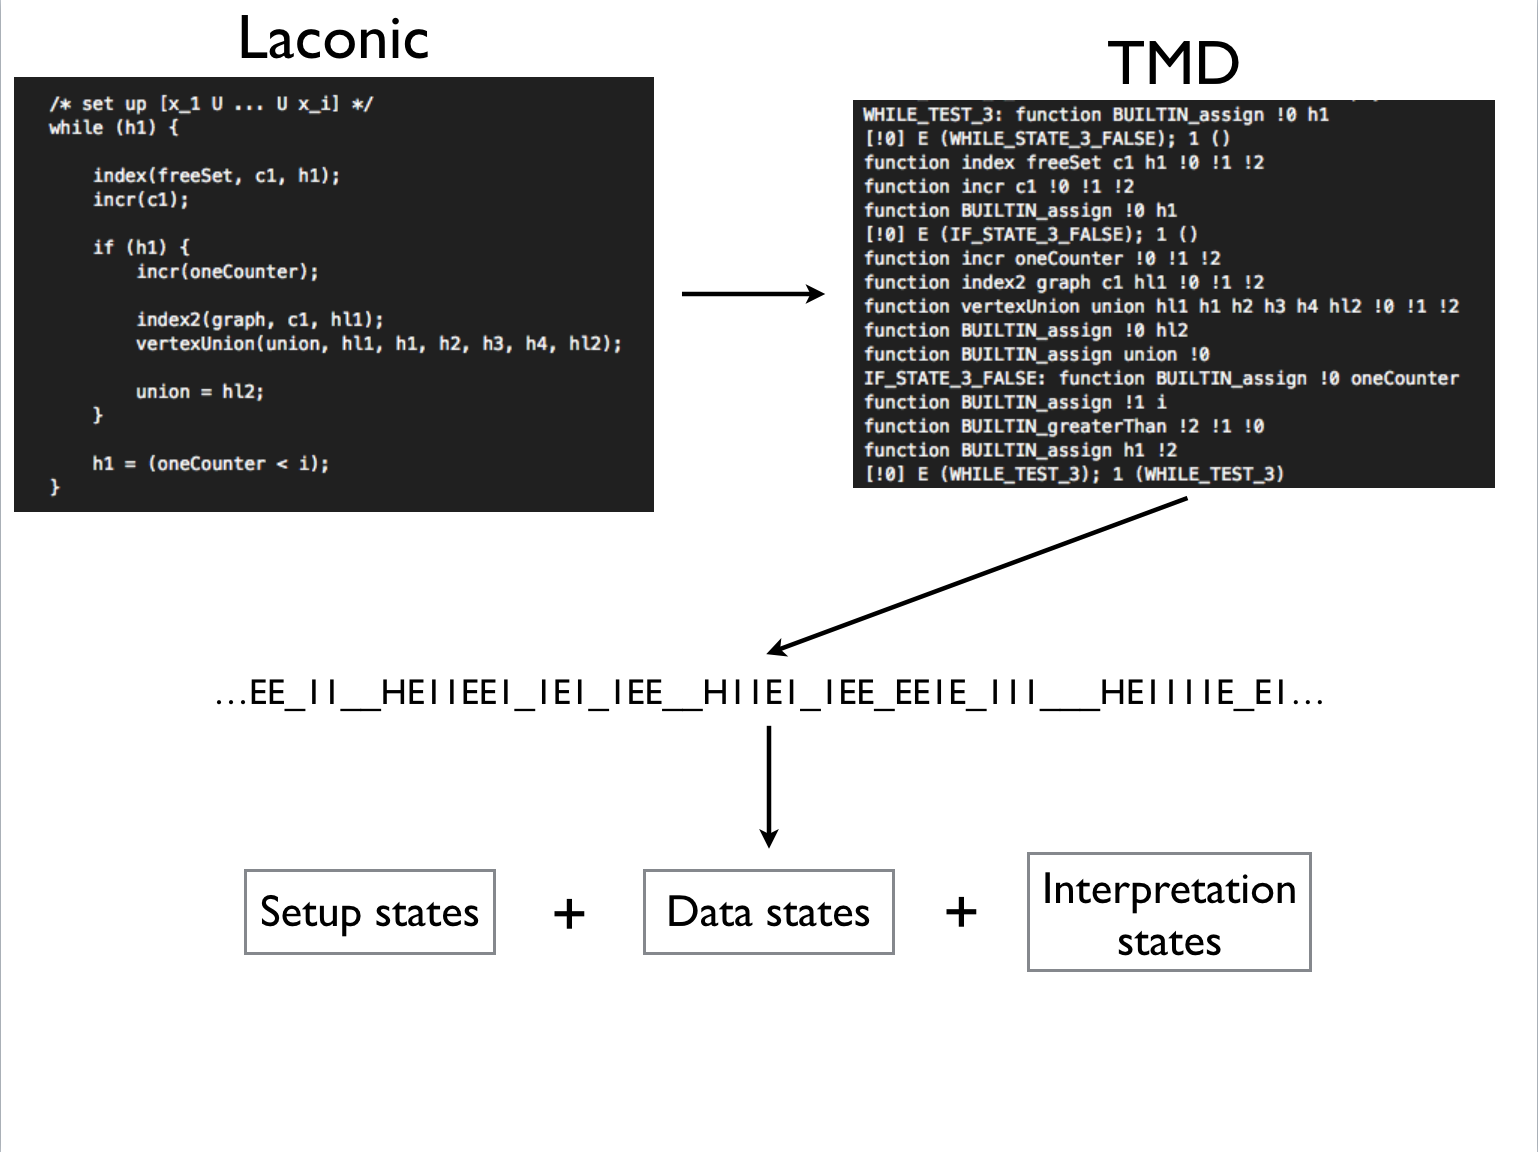
\includegraphics[scale=0.42]{figs/compilation.png}
\caption{A visual overview of the compilation process. \label{fig:compilation}} 
\end{center} 
\end{figure}

We recommend that programmers hoping to use our tools to generate their own encodings of mathematical statements or algorithms as Turing machines use Laconic. Laconic's interface is perfect for somebody hoping to write in a ``traditional'' language. On the other hand, if the programmer wishes to improve upon Laconic's compilation process, writing code directly in TMD is likely to be the better option.

\section{Related Work}

This paper is not the first to attempt to quantify the complexity of arithmetical statements. Calude and Calude~\cite{calude} define a register machine of their own design, and provide quantifications of the complexity of Legendre's conjecture, Fermat's last theorem, Goldbach's conjecture, Dyson's conjecture, the Riemann hypothesis, and the four color theorem.\footnotemark
\footnotetext{Because Fermat's last theorem and the four color theorem have been proved, their complexity is now known to be 0.}
In addition, Koza~\cite{koza} and Pargellis~\cite{pargellis} each invent instruction sets that are particularly well-suited to representing self-reproducing programs simply, and show that starting from a ``primordial soup'' of such instructions distributed about a large memory, along with an increasing number of program threads, a rich ecosystem of increasingly efficient self-reproducing programs start to dominate the ``landscape.'' 

This paper differs from the previous work in two ways: firstly, it is the first to give explicit, relatively small machines whose behavior is provably independent of the standard axioms of modern mathematics. Secondly, to our knowledge, this paper is the first concrete study of parsimony to use Turing machines as the model of computation---rather than (for example) a new programming language proposed by the authors! We consider it important to use the weakest and most common model of computation for complexity comparisons across different mathematical statements. This is because the more powerful and complex the model of computation used, the more of the complexity of the algorithm can be ``shunted'' onto the model of computation, and the greater the potential distortion created by the choice of model. As a reductio ad absurdum, we could imagine a programming language that included ``test the Riemann hypothesis'' and ``test the consistency of ZFC'' as primitive operations. By using the ``weakest'' model of computation that is commonly known, and one which is generally accepted as the mathematical basis of algorithms, we hope to avoid this pitfall and make it easier to interpret our results in a model-independent way.



\section{A Turing Machine that Cannot Be Shown to Run Forever Using ZFC}

We present a \statenumstate Turing machine whose behavior is \emph{independent of ZFC}; it would not be possible to prove that this machine would halt or wouldn't halt using the axioms of ZFC, assuming a slightly stronger set theory is consistent. It is therefore impossible to prove the value of \bbstatenum to be any given value without assuming axioms more powerful than ZFC, assuming that ZFC is consistent.

For an explicit listing of this machine, see Appendix~\ref{sec:explicitz}. 

We call this machine $Z$. One way to build this machine would be to start with the axioms of ZFC and apply the inference rules of first-order logic repeatedly in each possible way so as to enumerate every statement ZFC could prove, and to halt if ever a contradiction was found. While this method is conceptually simple, to actually construct such a machine would lead to a huge number of states, because it would require writing a program to manipulate the axioms of ZFC and the inference rules of first-order logic, and then compiling that program all the way down to Turing machine states. 

\subsection{Friedman's Mathematical Statement} \label{sec:friedmanstate}

Thankfully, a simpler method exists for creating $Z$. Friedman~\cite{friedman}
was able to derive a graph-theoretic statement whose truth implies the consistency of ZFC, and which will be false if ZFC is inconsistent.\footnotemark
\footnotetext{In fact, Friedman's statement is equivalent to the consistency of SRP (``stationary Ramsey property''), which is a system of axioms more powerful than ZFC. Because SRP is strictly more powerful than ZFC (it in fact consists of ZFC plus some additional axioms), the consistency of SRP implies the consistency of ZFC, and the inconsistency of ZFC implies the inconsistency of SRP.}
Here is Friedman's statement (the notation will be explained in the rest of this section): 

\begin{statement} \label{eq:friedman}
For all $k, n, r > 0$, every order invariant graph on $[\mathbb{Q}]^{\le k}$ has a free $\{x_1,\dots,x_r, \\
\textrm{ush}(x_1),...,\textrm{ush}(x_r)\}$ of complexity $\le (8knr)!$, each $\{x_1, \dots, x_{(8kni)!}\}$
reducing $[x_1 \cup \dots \cup x_i \cup \{0,\dots,n\}]^{\le k}$. \cite{friedman}
\end{statement}

A number of \emph{complexity} at most $c$ refers to a number that can be written as a fraction $a/b$, where $a$ and $b$ are both integers less than or equal to $c$. A set has complexity at most $c$ if all the numbers it contains have complexity at most $c$.  

An \emph{order invariant graph} is a graph containing a countably infinite number of nodes. In particular, it has one node for each finite set of rational numbers. The only numbers relevant to the statement are numbers of complexity $(8knr)!$ or smaller. In every description of nodes that follows, the term \emph{node} refers both to the object in the order invariant graph and to the set of numbers that it represents. 

In an order invariant graph, two nodes $(a,b)$ have an edge between them if and only if each other pair of nodes $(c,d)$ that is \emph{order equivalent} with $(a,b)$ has an edge between them. Two pairs of nodes $(a, b)$ and $(c, d)$ are \emph{order equivalent} if $a$ and $c$ are the same size and $b$ and $d$ are the same size and if for all $1 \le i \le |a|$ and $1 \le j \le |b|$, the $i$-th element of $a$ is less than the $j$-th element of $b$ if and only if the $i$-th element of $c$ is less than the $j$-th element of $d$. 

To give some trivial examples of order invariant graphs: the graph with no edges is order invariant, as is the complete graph. A less trivial example is a graph on $[\mathbb{Q}]^2$, in which each node corresponds to a set of two rational numbers of a given complexity, and there is an edge between two nodes if and only if their corresponding sets $a$ and $b$ satisfy $a_1 < b_1 < a_2 < b_2$. (Because edges are undirected in order invariant graphs, such an edge will exist if \emph{either} assignment of the vertices to $a$ and $b$ satisfies the inequality above). 

The \emph{ush()} function takes as input a set and returns a copy of that set with all non-negative numbers in that set incremented by 1. 

For vertices $x$ and $y$, $x \le_{rlex} y$ if and only if $x = y$ or $x_i < y_i$ where $i$ is least such that $x_i \not= y_i$.

Finally, a set of vertices $X$ \emph{reduces} a set of vertices $Y$ if and only if for all $y \in Y$, there exists $x \in X$ such that $x \le_{rlex} y$ and an edge exists between $x$ and $y$. 

\subsection{Implementation Methods}

To create $Z$, we needed to design a Turing machine that halts if Statement~\ref{eq:friedman} is false, and loops if Statement~\ref{eq:friedman} is true. Such a Turing Machine's behavior would necessarily be independent of ZFC, because the truth or falsehood of Statement~\ref{eq:friedman} is independent of ZFC, assuming the consistency of SRP, a slightly more powerful set theory.~\cite{friedman} 

To design such a Turing machine, we wrote a Laconic program which encoded Friedman's statement, then compiled the program down to a description of a single-tape, 2-symbol Turing machine. What follows is an extremely brief description of the design of the Laconic program; for the documented Laconic code itself, along with a detailed explanation of the full compilation process, please see~\cite{github}. 

Our Laconic program begins by looping over all non-negative values for $k$, $n$, and $r$. For each trio $(k, n, r)$, our program generates a list $N$ of all numbers of complexity at most $(8knr)!$. These numbers represent the vertices in our putative order invariant graph. Because Laconic does not support floating-point numbers, the list is entirely composed of integers; it is a list of all numbers that can be written in the form $(((8knr)!)!)((8kni)!)/((8knj)!)$, where $i$ and $j$ are integers satisfying $-(8knr)! \le i \le (8knr)!$ and $1 \le j \le (8knr)!$. (Note that any number that can be expressed in this form is necessarily an integer, because of the large scaling factor in front.) 

After we generate $N$, we generate the nodes in a potential order invariant graph by adding to $N$ all possible lists of $k$ or fewer numbers from $N$. We call this list of lists $V$. 

We iterate over all binary lists of length $|V|^2$. Any such list $E$ represents a possible set of edges in the graph. To be more precise, we say that an edge exists between node $i$ and node $j$ (represented by $V_i$ and $V_j$ respectively) if and only if $E_{i|V| + j}$ is 1. 

For any graph $(V, E)$, we say that it is ``valid'' if the following three conditions hold:

\begin{enumerate}

\item No node has an edge to itself.
\item If an edge exists between node $i$ and node $j$, an edge also exists between node $j$ and node $i$.
\item The graph has a free $\{x_1,\dots,x_r, \textrm{ush}(x_1),...,\textrm{ush}(x_r)\}$, each  $\{x_1, \dots, x_{(8kni)!}\}$ reducing $[x_1 \cup \dots \cup x_i \cup \{0,\dots,n\}]^{\le k}$.

\end{enumerate}

For each list of nodes $V$, we loop over every possible binary list $E$, and if no pair $(V, E)$ yields a valid graph, we halt. 

When verifying the validity of a graph, checking the first two conditions is trivial, but the third merits further explanation. In order to verify that a given graph $(V, E)$ has a free \\ $\{x_1,\dots,x_r, ush(x_1),...,ush(x_r)\}$, each  $\{x_1, \dots, x_{(8kni)!}\}$ reducing $[x_1 \cup \dots \cup x_i \cup \{0,\dots,n\}]^{\le k}$, we look at every possible subset of the nodes in $V$. For each subset, we verify that it has length $r$, that $\textrm{ush}(x_1),...,\textrm{ush}(x_r)$ all exist in $V$, and for each $i$ such that $(8kni)! \le r$, that $\{x_1, \dots, x_{(8kni)!}\}$ reduces $[x_1 \cup \dots \cup x_i \cup \{0,\dots,n\}]^{\le k}$. Once we have found such a subset, we know that the third conditon is satisfied.

{\color{red} I want to argue that the home for the paragraph from Appendix C about actually running the machine belongs in Appendix C instead of here. First, I think that the paragraph is not as technically ``serious'' as the rest of the material in this subsection. Second, I think that we're likely to have two sorts of readers: ``mathematicians'' and ``engineers.'' This subsection definitely belongs to the mathematicians; Appendix C, with its goofy font and giant list of states, is the home of the engineers. Mathematicians won't care what happens when you run the Turing machine, but engineers will be curious to hear if we tried it. And the paragraph fits nicely in Appendix C, since we're talking about the nitty-gritty details of $Z$.}

\section{A Turing Machine that Encodes Goldbach's Conjecture} \label{sec:g}

We present a \gbstatenumstate Turing machine that \emph{encodes Goldbach's conjecture}; in other words, to know whether this machine halts is to know whether Goldbach's conjecture is true. It is therefore impossible to prove the value of \bbgbstatenum without simultaneously proving or disproving Goldbach's conjecture.

Recall that Goldbach's conjecture is as follows:

\begin{statement}
\emph{Every even integer greater than 2 can be expressed as the sum of two primes.}
\label{goldbachstatement}
\end{statement}

Because Goldbach's conjecture is so simple to state, the Laconic program encoding the statement is also quite simple. It can be found in Appendix~\ref{sec:applac}. A detailed explanation of the compilation process, documentation for the Laconic language, and an explicit description of this Turing machine are available at~\cite{github}.

\section{A Turing Machine that Encodes Riemann's Hypothesis}

We present a \rmstatenumstate Turing machine that \emph{encodes Riemann's hypothesis}; in other words, to know whether this machine halts is to know whether Riemann's hypothesis is true. An explicit description of this machine can be found at~\cite{github}

Riemann's hypothesis is traditionally stated as follows:

\begin{statement}
\emph{The Riemann zeta function has its zeros only at the negative even integers and the complex numbers with real part 1/2.}
\label{goldbachstatement}
\end{statement}

\subsection{Equivalent Statement}

Instead of encoding the Riemann zeta function into a Laconic program, it is simpler to use the following statement, which was shown by Lagarias to be equivalent to the Riemann hypothesis~\cite{riemann}:

\begin{statement} \label{eq:riemann}
For all integers $n \ge 1$, 
$$\left(\left(\sum_{k \le \delta(n)} \frac{1}{k}\right) - \frac{n^2}{2}\right)^2 < 36n^3$$
\end{statement}

The function $\delta(n)$ used in Statement~\ref{eq:riemann} is defined as follows: 

\begin{nscenter}
$\eta(j) = p$ if $j = p^k$, $p$ is prime, $k$ is a positive integer \\
$\eta(j) = 1$ otherwise
\end{nscenter}
$$\delta(x) = \prod_{n<x}\prod_{j \le n} \eta(j)$$

\subsection{Implementation Methods}

This statement is equivalent to the following statement, which contains only positive integers\footnotemark:
\footnotetext{Although it is not immediately obvious at first glance, $\frac{\delta(n)!}{k}$ is necessarily an integer for all $k \le \delta(n)$, and $\frac{\delta(n)!}{2}$ is an integer for all $n > 1$.}

$$l(n) < r(n)$$ for all positive integers $n$, where

$$l(n) = (a(n))^2 + (b(n))^2$$
$$r(n) = 36n^3(\delta(n)!)^2 + 2a(n)b(n)$$.
$$a(n) = \sum_{k \le \delta(n)} \frac{\delta(n)!}{k}$$
$$b(n) = n^2\frac{\delta(n)!}{2}$$

To check the Riemann hypothesis, our program computes $a(n)$, $b(n)$, $l(n)$, and $r(n)$, in that order, for each possible value of $n$. If $l(n) \ge r(n)$, our program halts.

\section{Laconic}

Laconic is a programming language designed to be both user-friendly and easy to compile down to parsimonious Turing machine descriptions. 

Laconic is a strongly-typed language that supports recursive functions. Laconic compiles to an intermediate language called TMD. TMD programs are spread across multiple files and grouped into directories. TMD directories are meant to represent a sequence of commands that could be given to a multi-tape, 3-symbol Turing machine, using the Turing machine abstraction that allows the machine to read and write from one head at a time. 

For an example of a Laconic program, see Appendix~\ref{sec:applac}. For a visual illustration of the compilation process, see Figure~\ref{fig:compilation}.

\section{TMD}

TMD is a programming language designed to help the user describe the behavior of a multi-tape, 3-symbol Turing machine with a function stack. Each tape is infinite in one direction and supports three symbols: \texttt{\_}, \texttt{1}, and \texttt{E}. The blank symbol is \texttt{\_}: that is, \texttt{\_} is the only symbol that can appear on the tape an infinite number of times. The tape must always have the form $\texttt{\_}?(1|E)^+\texttt{\_}^{\infty}$; in other words, each tape must always contain a string of \texttt{1}'s and \texttt{E}'s of size at least 1, possibly preceded by a \texttt{\_} symbol, and necessarily followed by an infinite number of copies of the \texttt{\_} symbol. 

What is the purpose of having a language like TMD as an intermediary between Laconic and a description of a single-tape machine? The concept of tapes in a multi-tape Turing machine and the concept of variables in standard imperative programming languages map to one another very nicely. The idea of the Laconic-to-TMD compiler is to encode the value of each variable on one tape. Then, each Laconic command that manipulates the value of one or more variables compiles down to a TMD function call that manipulates the tapes that correspond to those variables appropriately. 

As an example, consider the following Laconic command: \\ \\
\texttt{a=b*c;} \\

This Laconic command assigns the value of \texttt{a} to the value of \texttt{b*c}. It compiles down to the following TMD function call: \\ \\
\texttt{function BUILTIN\_multiply a b c} \\

This function call will result in \texttt{BUILTIN\_multiply} being run on the three tapes \texttt{a}, \texttt{b}, and \texttt{c}. This will cause the symbols on tape \texttt{a} to take on a representation of an integer whose value is equal to $bc$.

In turn, the TMD code compiles directly to a string of bits that are written onto the tape at the start of the Turing machine's execution.

A TMD directory consists of three types of files:

\begin{enumerate}
\item The \texttt{functions} file. This file contains a list of the names of all the functions used by the TMD program. The top function in the file is pushed onto the stack at initialization. Moreover, when this top function returns, the Turing machine halts.
\item The \texttt{initvar} file. This file contains the non-\texttt{\_} symbols that start in each register at initialization. 
\item Any files used to describe TMD functions. These files all end in a \texttt{.tfn} extension and only have any relevance to the compiled program if they show up in the functions file.
\end{enumerate}

\section{Compilation and Processing}

When discussing the layout of the tape symbols and patterns, there are two ways to think about it: one is with a 4-symbol alphabet ($\{\texttt{\_}, \texttt{1}, \texttt{H}, \texttt{E}\}$, blank symbol \texttt{\_}), and one is with a 2-symbol alphabet ($\{\texttt{a}, \texttt{b}\}$, blank symbol \texttt{a}). The 2-symbol alphabet version is the one that's ultimately used for the results in this paper, since we advertised a Turing machine that used only two symbols. However, in nearly all parts of the Turing machine, the 2-symbol version of the machine is a direct translation of the 4-symbol version, according to the following mapping:

\begin{itemize}
\item $\texttt{\_} \leftrightarrow \texttt{aa}$
\item $\texttt{1} \leftrightarrow \texttt{ab}$
\item $\texttt{H} \leftrightarrow \texttt{ba}$
\item $\texttt{E} \leftrightarrow \texttt{bb}$
\end{itemize}

Additionally, the sections that follow may make reference to the \texttt{ERROR} state. Transitions to the \texttt{ERROR} state are stand-ins for transitions that should never be taken under any circumstances and are useful for debugging purposes.

\subsection{Concept} \label{sec:ontape}

A directory of TMD functions is converted at compilation time to a string of bits to be written onto the tape, along with other states designed to interpret these bits. The resulting Turing machine has three main components, or \emph{submachines}:

\begin{enumerate}
\item The \emph{initializer} sets up the basic structure of the variable registers and the function stack.
\item The \emph{printer} writes down the binary string that corresponds to the compiled TMD code.
\item The \emph{processor} interprets the compiled binary, modifying the variable registers and the function stack as necessary.
\end{enumerate}

The Turing machine's control flow proceeds from the initializer to the the printer to the interpreter. In other words, initializer states point only to initializer states or to printer states, printer states point only to printer states or to interpreter states, and interpreter states point only to interpreter states or the \texttt{HALT} state. 

This division of labor, while seemingly straightforward, actually constitutes a very important and non-obvious idea. The problem of the compiler is to convert a higher-level representation---a machine with many tapes, a larger alphabet, and a function stack---to the lower-level representation of a machine with a single tape, a 2-symbol alphabet and no function stack. The immediately obvious solution, and the one taught in every computability theory class as a proof of the equivalence of different kinds of Turing machines, is to have every ``state'' in the higher-level machine compile down to many states in the lower-level machine. %See Figure~\ref{fig:mttost} for a visual representation of what such a conversion might look like. 

While simple, this approach is suboptimal in terms of the number of states. As is nearly always true when designing systems to be parsimonious, the clue that improvement is possible lies in the presence of repetition. Each state transition in the higher-level machine is converted to a group of lower-level states with the same basic structure. Why not instead explain how to perform this conversion exactly once, and then apply the conversion many times?

This idea is at the core of the division of labor described previously. We begin by writing a description of the higher-level machine onto the tape, and then ``run'' the higher-level machine by reading what is on the tape with a set of states that understands how to interpret the encoded higher-level machine. We refer to this idea as \emph{on-tape processing}.

In this paper, we use TMD as the representation of the higher-level machine.\footnotemark
\footnotetext{Note that instead of TMD, the on-tape processing scheme could be used for any language, assuming the designer provides both a processor and an encoding for that language. We chose TMD because it made the interpreter easy to write, but other minimalist languages, like Unlambda~\cite{unlambda}, Brainf*ck~\cite{brainfuck}, or Iota and Jot~\cite{iota}, might be good candidates for parsimonious designs, with the additional advantage of being already known to some programmers! Thanks to Luke Schaeffer for this point. {\color{red} I don't think these languages need to be mentioned in the Related Work section---they have little to do with the Busy Beaver sequence or parsimony in general. They're just languages with very few primitives.}}
The printer writes the TMD program onto the tape, and the processor executes it. As a result of using this scheme, we incur a constant \emph{additive} overhead---we have to include the processor in our final Turing machine---but we avoid the constant \emph{multiplicative} overhead required for the na\"ive scheme. 

Is this additive overhead small enough to be worth it? We found that it is. Our implementation of the processor requires 3,860 states. (See Section~\ref{sec:cost} for a detailed breakdown of the state cost by submachine.) In contrast to this additive overhead of 3,860, the na\"ive approach incurs a large multiplicative overhead that depends in part on how many states must be used to represent each higher-level state transition, and in part on how efficient an encoding scheme can be devised for the on-tape approach. The following table compares the performance of on-tape processing to the performance of an implementation that used the na\"ive approach. The comparison is shown for three kinds of machines: a machine that halts if and only if Goldbach's conjecture is false, a machine that halts if and only if the Riemann hypothesis is false, and a machine whose behavior is independent of ZFC. 

\begin{center}
    \begin{tabular}{||c c c||}
    \hline
    Program & States (Na\"ive) & States (On-Tape Processing) \\ [0.5ex]
    \hline
    Goldbach & 7,902 & \gbstatenum\\
    \hline
    Riemann & 36,146 & \rmstatenum\\
    \hline 
    ZFC & 340,943 & \statenum\\
    \hline
    \end{tabular}
\end{center}

As can be seen from this table, on-tape interpretation results in huge gains, particularly in large and complex programs. 

The subsections that follow describe each of the three submachines---the initializer, the printer, and the processor---in greater detail.
 
\subsection{The Initializer}

The initializer starts by writing a counter onto the tape which encodes how many registers there will be in the program. Using the value in that counter, it creates each register, with demarcation patterns between registers, and unique identifiers for each register. Each register's value begins with the pattern of non-\texttt{\_} symbols laid out in the \texttt{initvar} file. The initializer also creates the program counter, which starts at 0, and the function stack, which starts out with only a single function call to the top function in the \texttt{functions} file.

Figure~\ref{fig:postinit} is a detailed diagram describing the tape's state when the initializer passes control to the printer. 

\begin{figure} 
\begin{center} 
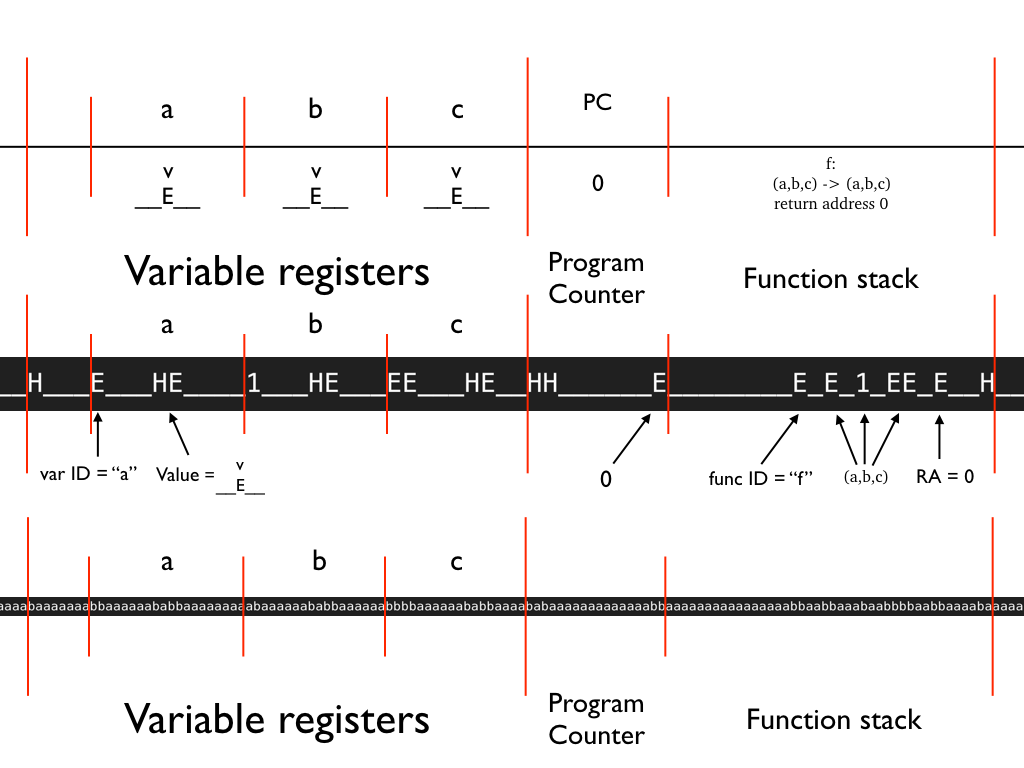
\includegraphics[scale=0.42]{figs/postinit.png}
\caption{The state of the Turing machine tape after the initializer completes. The TMD program being expressed in Turing machine form is described in full in Appendix~\ref{sec:apptmd}. The top bar is a high-level description of what each part of the Turing machine tape represents. The middle bar is an encoding of the tape in the standard 4-symbol alphabet; the bottom bar is simply the translation of that tape into the 2-symbol alphabet. For a more detailed explanation of how to interpret the tape patterns, see~\cite{github}. \label{fig:postinit}} 
\end{center} 
\end{figure}

\subsection{The Printer} \label{sec:introspect}

\subsubsection{Specification}

The printer writes down a long binary string which encodes the entirety of the TMD program onto the tape.

Figure~\ref{fig:postprog} is a detailed diagram describing the tape's state when the printer passes control to the processor.

\begin{figure}
\begin{center}
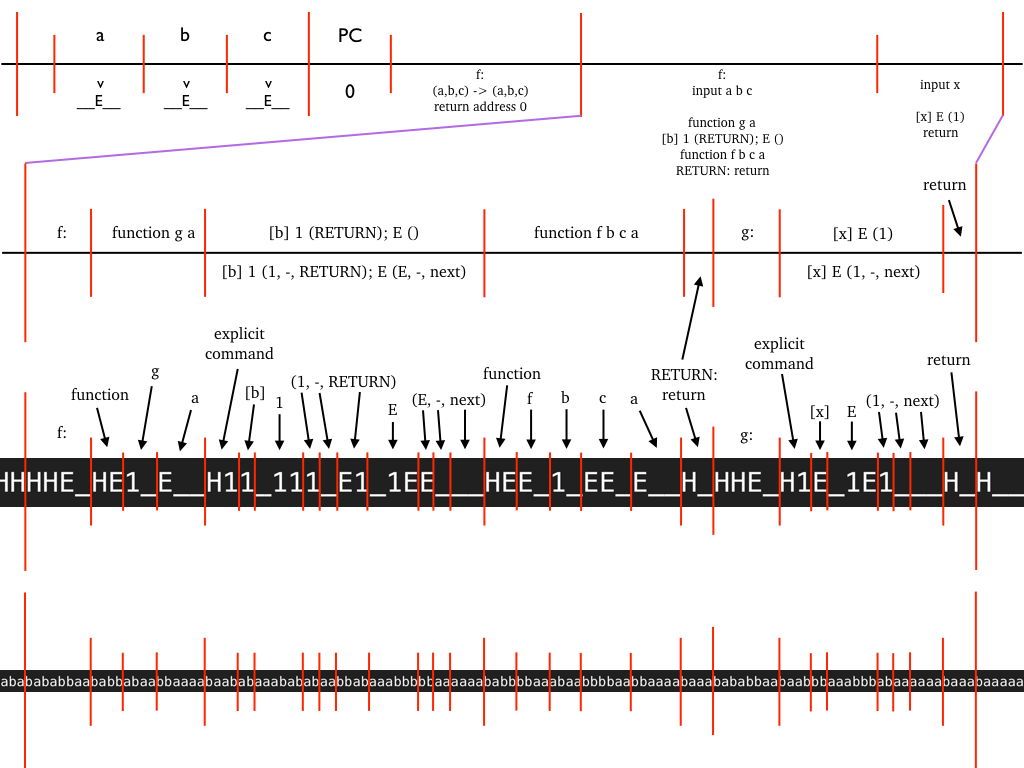
\includegraphics[scale=0.42]{figs/postprog.png}
\caption{The state of the Turing machine tape after the printer completes. The TMD program being expressed in Turing machine form is described in full in Appendix~\ref{sec:apptmd}. The top bar is a high-level description of the entire tape; unfortunately, at this point there are so many symbols on the tape that it is impossible to see everything at once. For a detailed view of the first two-thirds of the tape (registers, program counter, and stack), see Figure~\ref{fig:postinit}. The bottom three bars show a zoomed-in view of the program binary. From the top, the second bar gives a high-level description of what each part of the program binary means; the third bar gives the direct correspondence between 4-symbol alphabet symbols on the tape and their meaning in TMD; the fourth and final bar gives the translation of the third bar into the 2-symbol alphabet. For a more detailed explanation of the encoding of TMD into tape symbols, see~\cite{github}. \label{fig:postprog}}
\end{center}
\end{figure}

\subsubsection{Introspection}

Writing down a long binary string onto a Turing machine tape in a parsimonious fashion is not as straightforward as it might initially appear. The first idea that comes to mind is simply to use one state per symbol, with each state pointing to the next, as shown in Figure~\ref{fig:naiveprog}. 

\begin{figure}
\begin{center}
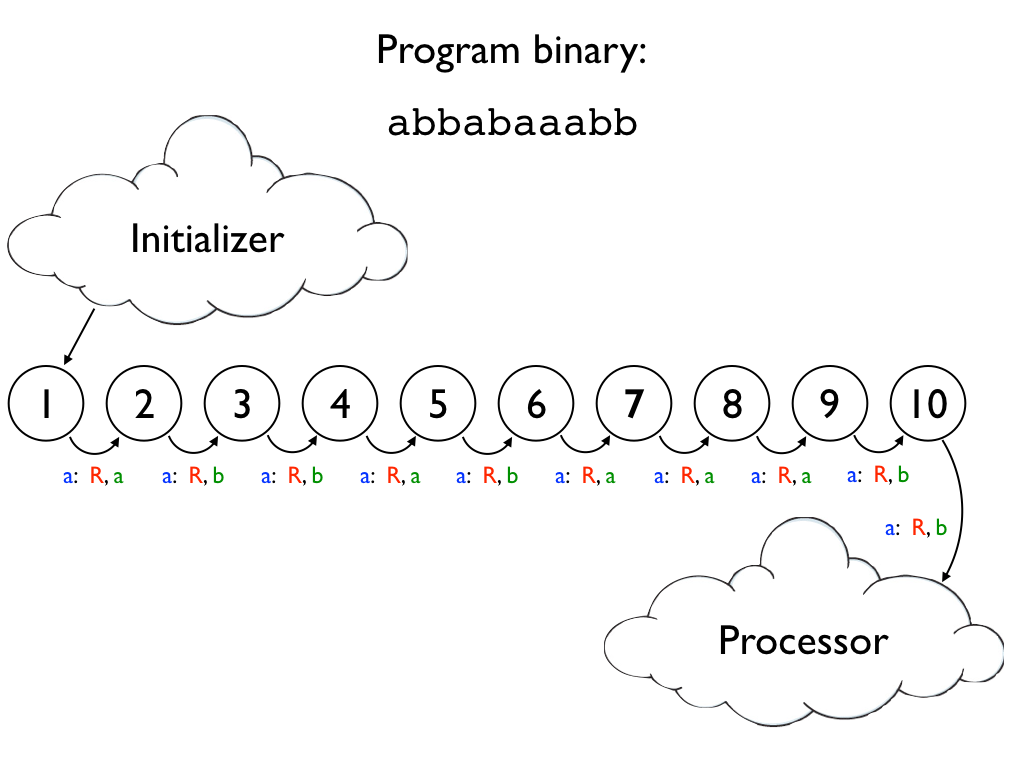
\includegraphics[scale=0.28]{figs/naiveprog.png}
\caption{A na\"ive implementation of the printer. In this example, the hypothetical program is ten bits long, and the printer uses ten states, one for each bit. In the diagram, the blue symbol is the symbol that is read on a transition, the red letter indicates the direction the head moves, and the green symbol indicates the symbol that it written. Note the lack of transitions on reading a \texttt{b}; this is because in this implementation, the printer will only ever read the blank symbol, which is \texttt{a}, since the head is always proceeding to untouched parts of the tape. It therefore makes no difference what behavior the Turing machine adopts upon reading a \texttt{b} in states 1-10 (and therefore \texttt{b} transitions are presumed to lead to the \texttt{ERROR} state) \label{fig:naiveprog}}
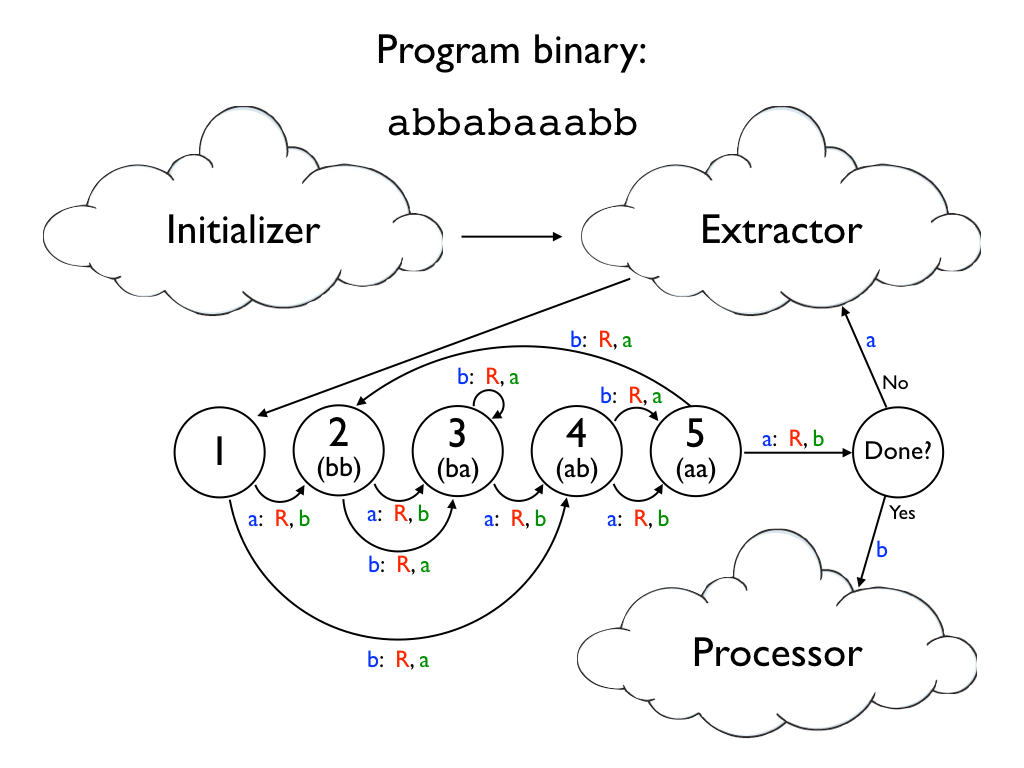
\includegraphics[scale=0.28]{figs/introspectprog.png}
\caption{An introspective implementation of the printer. In this example, the hypothetical program is $k=10$ bits long, and so the word size must be 2 (since $w=2$ is the largest $w$ such that $w2^w \le 10$). There are therefore $n_w = \left \lceil{\frac{k}{w}}\right \rceil = 5$ data states, each encoding two bits. The \texttt{b} transitions carry the information about the encoding; note that each one only points to one of the last four data states. The last four data states have in parentheses what word we mean to encode if we point to them. \label{fig:introspectprog}}
\end{center}
\end{figure}

Upon closer examination, however, it is apparent that this approach is quite wasteful for all but the smallest binary files. Every \texttt{a} transition points to the next state in the sequence, and none of the \texttt{b} transitions are used at all! Indeed, the only information-bearing part of the state is the single bit contained in the choice of which symbol to write. But in theory, far more information than that could be encoded with each state. In a machine that contains $n$ states, each state could contain $2(\log(n) + 1)$ bits of information, because each of its two transitions could point to any of the $n$ states, and write either an \texttt{a} or a \texttt{b} onto the tape. Of course, this is only in theory; in practice, to extract the information contained in the Turing machine's states and translate it into bits on the tape is nontrivial. 

What we propose here is a scheme originally conceived by Ben-Amram and Petersen~\cite{benamram} and refined further and suggested to us by Luke Schaeffer. It does not achieve the optimal theoretical encoding described above, but is relatively simple to implement and understand, and is within a factor of 2 of optimal for large binary strings. Schaeffer named Turing machines that use this idea \emph{introspective}.  

Introspection works as follows. If the binary string contains $k$ bits, then let $w$ be the \emph{word size}. $w$ takes the largest value it can such that $w2^w \le k$. We can split the binary string into $n_w = \left \lceil{\frac{k}{w}}\right \rceil$ different \emph{words} of size $w$ bits each (we can pad the last word with copies of the blank symbol). In our scheme, each word in the bit-string will be represented by a \emph{data state}. Each data state points to the state representing the next word in the sequence for its \texttt{a} transition, but which state the \texttt{b} transition points will encode the next word. Every \texttt{b} transition points to one of the last $2^w$ data states, thereby encoding $w$ bits of information. 

Of course, the encoding is useless until we specify how to extract the encoded bit-string from the data states. The extraction scheme works as follows. To query the $i^\textrm{th}$ data state for the bits it encodes, we run the data states on the string $\texttt{a}^{i-1}\texttt{b}\texttt{a}^{\infty}$ (a string of $i-1$ \texttt{a}'s followed by a \texttt{b} in the $i^\textrm{th}$ position). After running the data states on that string, what remains on the tape is the string $\texttt{b}^{i-1}\texttt{a}\texttt{b}^r\texttt{a}^{\infty}$, assuming that the $i^\textrm{th}$ data state pointed to the $r^\textrm{th}$-to-last data state. Thus, what we are left with is essentially a unary encoding of the ``value'' of the word in binary. Thus, the job of the extractor is to set up a binary counter which removes one \texttt{b} at a time and increments the counter appropriately. Then, afterward, the extractor reverts the tape back to the form $\texttt{a}^i\texttt{b}\texttt{a}^{\infty}$, shifts all symbols on the tape over by $w$ bits, and repeats the process. Finally, when the state beyond the last data state sees a \texttt{b} on the tape, we know that the process has completed, and we can pass control to the processor. Figure~\ref{fig:introspectprog} depicts the introspection algorithm.

How much have we gained by using an introspective technique for encoding the program binary, instead of the na\"ive approach? It depends on how large the program binary is. By using introspection, we incur an $O(\log k)$ \emph{additive} overhead, because we have to include the extractor in our machine. (Our implementation of the extractor takes $10w + 17$ states.) But in return, we save a \emph{multiplicative} factor of $w$ (which scales with $\log k$) on the number of data states needed. 

This is plainly not worth it for the 10-bit example binary shown in Figs.~\ref{fig:naiveprog} and~\ref{fig:introspectprog}. For that binary, we require 69 additional states for the extractor in order to save 5 states on the data states. For real programs, however, it is worth it, as can be seen from the following table.

\begin{center}
    \begin{tabular}{||c c c c c c c||}
    \hline
    Program & Binary Size & $w$ & $n_w$ & Extractor Size & States (Na\"ive) & States (Introspective) \\ [0.5ex]
    \hline\hline
    Example TMD & 116 & 4 & 29 & 57 & 116 & 86 \\
    \hline
    Goldbach & 4,964 & 9 & 552 & 107 & 4,964 & 659 \\
    \hline
    Riemann & 9,532 & 10 & 1,024 & 117 & 9,532 & 1,141 \\
    \hline 
    ZFC & 35,906 & 11 & 3,265 & 127 & 35,906 & 3,392 \\
    \hline
    \end{tabular}
\end{center}

One minor detail concerns the numbers presented for the Riemann program. Ordinarily, with a binary of size 9,532, we would opt to split the program into 1,060 words of 9 bits each plus a 107-state extractor, since 9 is the greatest $w$ such that $w2^w <$ 9,532. But because 9,532 is so close to the ``magic number'' 10,240, it's actually more parsimonious to pad the program with copies of the blank symbol until it's 10,240 bits long, and split it into 1,024 words of 10 bits each plus a 117-state extractor.
{\color{red} It's okay to take the greatest $w$ such that $w2^w <$ 9,532, because we use $n_w = \left \lceil{\frac{9532}{w}}\right \rceil$ data states (and NOT $2^w$ data states, as I believe you are assuming, and which you correctly note would be insufficient to encode the whole bit-string). The scheme that I originally used was what you are suggesting (take the least $w$ such that $w2^w \ge$ 9,532, and use $2^w$ data states) but after I emailed as much to you and Luke, Luke pointed out that we could do better by a multiplicative factor between 1 and 2 by taking $w$ to be one smaller and just having more some extra data states that can't be pointed to; that way, you don't have all that wasted space at the end! (In fact, Luke's method is \emph{almost} always better than the one I originally suggest here and that you suggested in your comments, so what I actually do is check which of the two methods uses less states and use that one; that's what this paragraph is all about.)}


\subsection{The Processor}

The processor's job is to interpret the code written onto the tape and modify the variable registers and function stack accordingly. The processor does this by the following sequence of steps:  \\ \\
START:
\begin{enumerate}
\item Find the function call at the top of the stack. Mark the function $f$ in the code whose ID matches that of the top function call.
\item Read the current program counter. Mark the line of code $l$ in $f$ whose line number matches the program counter.
\item Read $l$. Depending on what type of command $l$ is, carry out one of the following three lists of tasks.
\end{enumerate}

IF $l$ IS AN EXPLICIT TAPE COMMAND:
\begin{enumerate}
\item Read the variable name off $l$. Index the variable name into the list of variables in the top function on the stack. This list of variables corresponds to the mapping between the function's local variables and the register names.
\item Match the indexed variable to its corresponding register $r$. Mark $r$. Read the symbol $s_r$ to the right of the head marker in that register.
\item Travel back to $l$, remembering the value of $s_r$ using states. Find and mark the reaction $x$ corresponding to the symbol. See what symbol $s_w$ should be written in response to reading $s_r$.
\item Travel back to $r$, remembering the value of $s_w$ using states. Replace $s_r$ with $s_w$.
\item Travel back to $x$. See which direction $d$ the head should move in response to reading $s_r$.
\item Travel back to $r$, remembering the value of $d$ using states. Move the head marker accordingly.
\item Travel back to $x$. See if a jump is specified. If a jump is specified, copy the jump address onto the program counter. Otherwise, increment the program counter by 1.
\item Go back to START.
\end{enumerate}

IF $l$ IS A FUNCTION CALL:
\begin{enumerate}
\item Write the function's name to the top of the stack.
\item For each variable in the function call, index the variable name into the list of variables in the top function on the stack. This list of variables corresponds to the mapping between the function's local variables and the register names. Push the corresponding register names in the order that they correspond to the variables in the function call. 
\item Copy the current program counter to the return address of the newborn function call at the top of the stack.
\item Replace the current program counter with 0 (meaning ``read the first line of code'').
\item Go back to START.
\end{enumerate}

IF $l$ IS A RETURN STATEMENT:
\begin{enumerate}
\item Replace the current program counter with $f$'s return address.
\item Increment the program counter by 1.
\item Erase the call to $f$ from the top of the stack.
\item Check if the stack is now empty. If so, halt.
\item Go back to START.
\end{enumerate}

\subsection{Cost Analysis} \label{sec:cost}

It is worthwhile to analyze the relative contributions of the initializer, the printer, and the processor to the machine's final state count. The following table lists the number of states in each submachine for each of the four different TMD programs under discussion. 

\begin{center}
    \begin{tabular}{||c c c c c||}
    \hline
    Program & Initializer & Printer & Processor & Total \\ [0.5ex]
    \hline\hline
    Example TMD & 349 & 86 & 3,860 & 4,295 \\
    \hline
    Goldbach & 369 & 659 & 3,860 & \gbstatenum \\
    \hline
    Riemann & 371 & 1,141 & 3,860 & \rmstatenum \\
    \hline 
    ZFC & 389 & 3,392 & 3,860 & \statenum \\
    \hline
    \end{tabular}
\end{center}

As can be seen from this table, the processor makes the largest contribution to all four programs. Improving the processor, therefore, is probably the best approach for improving upon the bounds we present. Equally clear, however, is that for programs more complicated than the ones presented here, the cost of the printer will grow almost linearly but the cost of the processor will stay the same. The cost of the initializer grows very slightly with the complexity of programs because of the need to initialize additional registers. 

Improving the printer, and with it the TMD and Laconic languages, is probably the best approach for reducing state count for very large and complex programs.

\section{Future Work}

How much further can $Z$'s state count be reduced? Without a significant new insight, further order-of-magnitude reductions seem unlikely via tweaks to our existing system: note that such tweaks would need to reduce the sizes of both the printer and the processor by an order of magnitude. However, improvement is possible by (for example) a redesigned processor, combined with a simpler independent mathematical statement than Friedman's. 

Other future work might involve further use of our Laconic language to upper-bound the `complexities' of mathematical statements and algorithms, in as standardized and model-independent a way as possible. Perhaps Laconic could be used to measure the complexity of other well-known conjectures, or even to compare different algorithms for solving the same problem to each other (e.g. to try to quantify the notion that an insertion sort is simpler than a merge sort)!

\section{Acknowledgements}

%First and foremost, I would like to acknowledge my advisor, Prof. Scott Aaronson, for having suggested this problem to me and for having provided me with indispensable aid throughout. Prof. Aaronson explained the finer points of set theory to me in great detail, and put a huge amount of time into helping me refine my writing into something readable. His kindness, his constant availability to talk, and his friendliness made this Master's thesis a great pleasure to write.

We thank Prof. Harvey Friedman for having done the crucial theoretical work that made this project feasible. Prof. Friedman was endlessly available over email, and provided us with immediate and detailed clarifications when we needed them.

We thank Luke Schaeffer for his early help, as well as his help designing introspective Turing machines. 

We thank Adam Hesterberg for his help explaining the meaning of various common mathematical terms used in Friedman's work. {\color{red} This sentence fits just fine in my thesis, but maybe it should be removed now that you are an author---I imagine that you would have understood the meaning of those mathematical terms just fine without asking Adam! \texttt{:)}} 

We thank Alex Arkhipov for introducing us to the term ``code golfing.''

Supported by an Alan T. Waterman Award from the National Science Foundation, under grant no. 1249349.

\begin{thebibliography}{100}
\bibitem{iota} Barker, C. ``Iota and Jot: the simplest languages?'' http://semarch.linguistics.fas.nyu.edu/barker/Iota/ [A website describing the Iota and Jot programming languages]
\bibitem{benamram} Ben-Amram, A., Petersen, H. ``Improved Bounds for Functions Related to Busy Beavers'' Theory of Computing Systems 35, 1-11 (2002) 
\bibitem{bbfour} Brady, A.H. ``Solution of the Non-computable `Busy Beaver' game for $k=4$.'' Abstracts for: ACM Computer Science Conference (Washington, DC, February 18-20, 1975), p. 27, ACM, 1975.
\bibitem{riemann} Browder, F. ``Mathematical Developments Arising from Hilbert Problems.'' American Mathematical Society. Volume 28, Part 1. {\color{red} I tried to find a page number for this, but among all the papers I found that cited this, nobody else provided a page number for some reason. Perhaps Part 1 of Volume 28 of the AMS only has one page in it?}
\bibitem{calude} Calude, C., Calude, E. ``Evaluating the Complexity of Mathematical Problems: Part 1,'' ``Evaluating the Complexity of Mathematical Problems: Part 2.'' Complex Systems 18, pp. 387-401. 2010.
\bibitem{friedman} Friedman, H. ``Order Invariant Graphs and Finite Incompleteness.'' https://u.osu.edu/friedman.8/files/2014/01/FIiniteSeqInc062214a-v9w7q4.pdf
\bibitem{friedmanlist} Friedman, H. ``Order Theoretic Equations, Maximality, and Incompleteness.'' June 7, 2014. http://u.osu.edu/friedman.8/foundational-adventures/downloadable-manuscripts \#78.
\bibitem{godelcohen} G\"odel, K. ``The Consistency of the Axiom of Choice and of the Generalized Continuum-Hypothesis with the Axioms of Set Theory.'' Published in 1940 by the Princeton University Press. Annals of Mathematics Studies.
\bibitem{koza} Koza, J. ``Spontaneous Emergence of Self-Replicating and Evolutionarily Self-Improving Computer Programs.'' in Artificial Life III (SFI Studies in the Sciences of Complexity, vol. XVII), C. G. Langton, Ed. Reading, MA: Addison-Wesley. pp. 225-262. 1994. 
\bibitem{bbsmall} Lin, S., Rado, T. ``Computer Studies of Turing Machine Problems.'' Published in Journal of the ACM, Volume 12, Issue 2, April 1965. Pages 196-212.
\bibitem{unlambda} Madore, D. ``The Unlambda Programming Language.'' http://www.madore.org/~david/programs/unlambda/ [A website describing the Unlambda programming language]
\bibitem{bbimpossible} Marxen, H., Buntrock, J. ``Attacking the Busy Beaver 5.'' Bull EATCS, Vol. 40, pp. 247-251. 1990. {\color{red} You wrote: ``Ref. [8] should probably have H. Marxen as the {`author.'}'' I'm unsure what you mean---haven't I already listed H. Marxen as the author here?}
\bibitem{brainfuck} M\"uller, U. ``Brainfuck.'' http://www.muppetlabs.com/~breadbox/bf/ [A website describing the Brainf*ck programming language]
\bibitem{pargellis} Pargellis, A. ``The Spontaneous Generation of Digital {`Life.'}'' Physica D, 91, 86-96. 1996.
\bibitem{busybeaver} Rado, T. ``On Non-Computable Functions.'' Bell System Technical Journal, 41: 3. May 1962 pp 877-884.
\bibitem{schoenfield} Schoenfield, J. ``The Problem of Predicativity.'' Essays on the foundations of mathematics, Y. Bar-Hillel et al., eds., pp. 132-142. 1961.
\bibitem{bbvalues} http://www.drb.insel.de/\symbol{126}heiner/BB/ [A list of the known busy beaver values]
\bibitem{codegolf} http://codegolf.stackexchange.com/ [A place where programmers go for recreational code golfing]
\bibitem{github} https://github.com/adamyedidia/parsimony A link to a GitHub repository containing all programs, Turing machines related to this paper, along with related documentation. 
\end{thebibliography}

\begin{appendices}
    
\section{Example Laconic Program: Goldbach's Conjecture} \label{sec:applac}

The following is an example Laconic program, which compiles down to the Turing machine $G$ mentioned in Section~\ref{sec:g} (which halts if and only Goldbach's Conjecture is false).

{\tiny \tt \noindent \onehalfspacing \parskip 0pt
func zero(x) \{ \\
\hspace{5mm} x = 0; \\
    return; \\
\} \\
\\
func one(x) \{ \\
    x = 1; \\
    return; \\
\} \\
\\
func incr(x) \{ \\
    x = x + 1; \\
    return; \\
\} \\
\\
/* Computes x modulo y */ \\
func modulus(x, y, out) \{ \\
    out = x; \\
\\    
    while (out >= y) \{ \\
        out = out - y; \\
    \} \\
\\     
    return; \\
\} \\
\\
func assignXtoYminusX(x, y) \{ \\
    x = y - x; \\
    return; \\
\} \\
\\
/* Figures out if x is prime, and puts the output in y */ \\
/* Does not modify x, modifies y */ \\
func isPrime(x, h, y) \{ \\
    if (x == 1) \{ \\ 
        zero(y); \\
        return; \\
    \} \\
\\    
    y = 2; \\
\\    
    while (x > y) \{ \\
        modulus(x, y, h); \\
\\    
        if (h == 0) \{ \\
            zero(y); \\
            return; \\
        \} \\
        incr(y); \\
    \} \\
\\    
    return; \\
\} \\
\\
int evenNumber; \\
int primeCounter; \\
int isThisOnePrime; \\
int foundSum; \\
int h; \\
\\
evenNumber = 2;\\
one(foundSum);\\
\\
while (foundSum) \{\\
    zero(foundSum);\\
    evenNumber = evenNumber + 2;\\
    one(primeCounter);\\
    \\
    while (primeCounter < evenNumber) \{\\    
        isPrime(primeCounter, h, isThisOnePrime);\\
        \\
        if (isThisOnePrime) \{\\
            assignXtoYminusX(primeCounter, evenNumber);\\
            isPrime(primeCounter, h, isThisOnePrime);\\
            assignXtoYminusX(primeCounter, evenNumber);\\
            \\
            if (isThisOnePrime) \{\\
                print evenNumber;\\
                print primeCounter;\\
                \\
                one(foundSum);\\
            \}\\
        \}\\
        \\
        incr(primeCounter);  \\
    \}         \\
\}\\
\\
halt;\\ }

For detailed documentation of the Laconic programming language, see~\cite{github}. To find this file specifically, navigate to \texttt{parsimony/src/laconic/laconic\_files/goldbach.lac} at~\cite{github}.

\section{Example TMD Program} \label{sec:apptmd}

The following is an example TMD directory, which compiles down to a binary string to be written on a Turing machine tape. It is the example that is used in illustrations throughout this paper, most notably in the example compilation shown in Figs.~\ref{fig:postinit} and~\ref{fig:postprog}. The program calls itself recursively three times until the starting symbol on each tape, \texttt{E}, is replaced with a \texttt{1}, at which point the program halts.

This TMD directory is called \texttt{example\_tmd\_dir}, and contains four files: \texttt{f.tmd}, \texttt{g.tmd}, \texttt{initvar}, and \texttt{functions}. \\ \\

\texttt{f.tmd}:
{ \scriptsize \tt
\begin{lstlisting}
input a b c

// Recursively writes a 1 on every tape.

function g a 
[b] 1 (RETURN); E ()
function f b c a
RETURN: return
\end{lstlisting}
}
\texttt{g.tmd}:
{ \scriptsize \tt
\begin{lstlisting}
input x

// Writes a 1 on the input tape.

[x] E (1)
return
\end{lstlisting}
}

\texttt{functions}:
../busybeaver/functions.tex
\texttt{initvar}:
{ \scriptsize \tt
\begin{lstlisting}
E
\end{lstlisting}
} 

For detailed documentation of the TMD programming language, see~\cite{github}. To find this directory specifically, navigate to \texttt{parsimony/src/tmd/tmd\_dirs/example\_tmd\_dir/} at~\cite{github}.

\section{Explicit Listing of $Z$} \label{sec:explicitz}

We present below an explicit listing of $Z$. For a more easily readable version of $Z$, complete with descriptive state names, see~\cite{github}. 

We ran this Turing Machine for 10,000,000,000 steps (more than half a day on our simulators) and within that time it did not halt. We note, however, that it was designed for parsimony and not for efficiency, and that this ``experiment'' is of little consequence! We similarly designed and ran a Turing machine designed to test the conjecture that all perfect squares are less than 5, and it ran for 2,895,083,899 steps (a couple hours on our simulators) before it found the counterexample 9 and halted.

{\color{red} See Section 3.2 for why I kept the paragraph here}

Figure~\ref{fig:syntax} presents useful information for how to interpret the description shown below. In addition, note the following:

\begin{enumerate}

\item The tape has a 2-symbol alphabet, with tape symbols $\{\texttt{a}, \texttt{b}\}$ and blank symbol \texttt{a} (in other words, \texttt{a} is the only symbol that can appear an infinite times on the tape).
\item The start state of $Z$ is \texttt{0000}.
\item $Z$ will never transition to the \texttt{ERROR} state. Any transition to the \texttt{ERROR} state could be replaced by a transition to any other state (including \texttt{HALT}) and the Turing machine's behavior would remain identical.
\item $Z$ contains only one transition to the \texttt{HALT} state, out of state \zhaltstate.

\end{enumerate}

\begin{figure} 
\begin{center} 
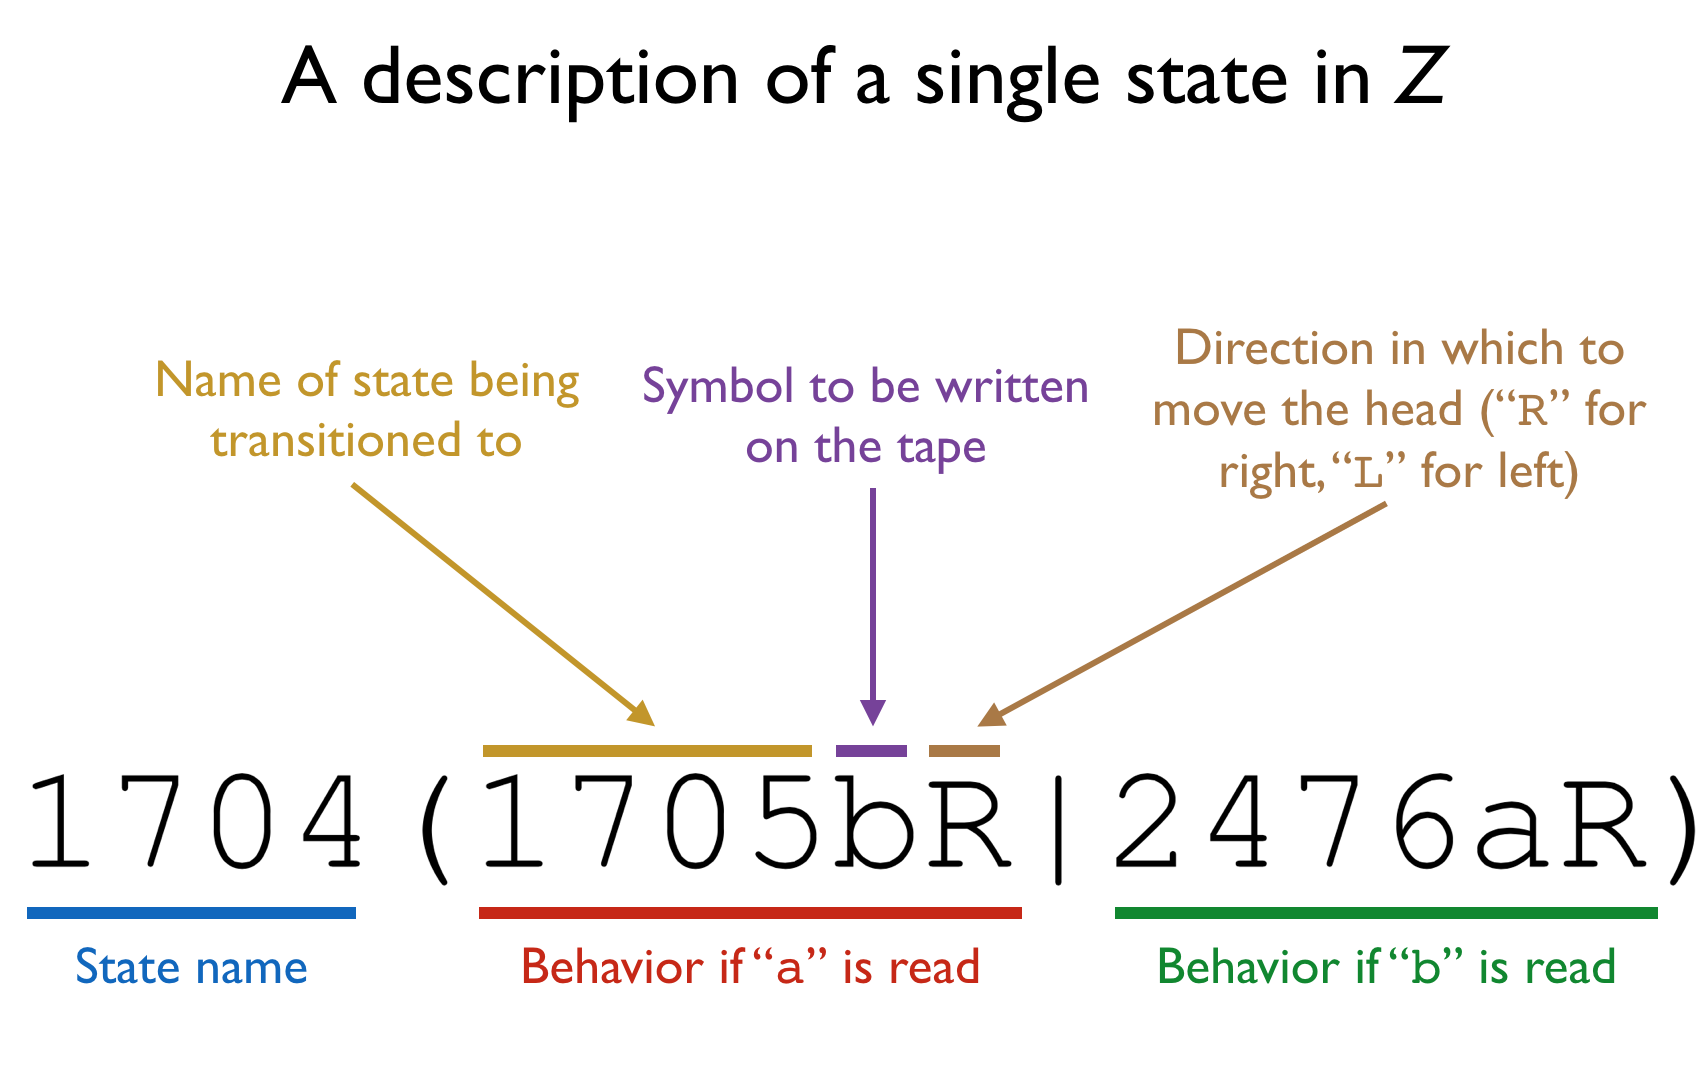
\includegraphics[scale=0.4]{figs/syntax.png}
\caption{This figure explains how to read a description of a single state. Note that ``\texttt{ERROR-}'' or ``\texttt{HALT--}'' denote transitions to the \texttt{ERROR} or \texttt{HALT} states, respectively (no further information is provided because what symbol is written and which direction the head moves are at that point irrelevant). \label{fig:syntax}} 
\end{center} 
\end{figure}
%\clearpage
\resizebox{17cm}{!}{\centering\tt\begin{tabular}{@{}l@{}}0000(0001bR|ERROR-) 0001(0004bR|ERROR-) 0002(0003bR|ERROR-) 0003(0012aR|0012bR) 0004(0005bR|ERROR-) 0005(0006bR|ERROR-) 0006(0007aR|ERROR-) 0007(0008bR|ERROR-) 0008(0009bR|ERROR-) \\0009(0010bR|ERROR-) 0010(0011bR|ERROR-) 0011(0002bR|ERROR-) 0012(0013aR|ERROR-) 0013(0014aR|0014bR) 0014(0015aR|ERROR-) 0015(0057aR|0057bR) 0016(0017bR|ERROR-) 0017(0018bR|ERROR-) \\0018(0019aR|ERROR-) 0019(0020aR|0020bR) 0020(0021aR|ERROR-) 0021(0022aR|0022bR) 0022(0023aR|ERROR-) 0023(0024aR|0024bR) 0024(0025aR|ERROR-) 0025(0067aR|0067bR) 0026(0027aR|0032bR) \\0027(0028aL|0030bL) 0028(0029aL|0029bL) 0029(0026aL|0026bL) 0030(0031aL|0031bL) 0031(0026aL|0026bL) 0032(0033aL|0035bL) 0033(0034aL|0034bL) 0034(0037aL|0037bL) 0035(0036aL|0036bL) \\0036(0026aL|0026bL) 0037(0038aR|0041bR) 0038(0044aR|0039bL) 0039(0040bR|0040bR) 0040(0049aL|0049bL) 0041(ERROR-|0042bL) 0042(0043aL|0043aL) 0043(0037aL|0037bL) 0044(0045aR|0048bR) \\0045(ERROR-|0046aL) 0046(0047aR|0047aR) 0047(0049aL|0049bL) 0048(0071aR|ERROR-) 0049(0050aR|0051bR) 0050(0049aR|0049bR) 0051(0052aR|0049bR) 0052(0053aR|0054bR) 0053(0052aR|0052bR) \\0054(0055aL|0052bR) 0055(0056aR|0056aR) 0056(0012aR|0012bR) 0057(0058aR|ERROR-) 0058(0059aR|0059bR) 0059(0060aR|ERROR-) 0060(0061aR|0061bR) 0061(0062aR|ERROR-) 0062(0063aR|0063bR) \\0063(0064aR|ERROR-) 0064(0065aR|0065bR) 0065(0066aR|ERROR-) 0066(0016aR|0016bR) 0067(0068bR|ERROR-) 0068(0069bR|ERROR-) 0069(0070bL|ERROR-) 0070(0026aL|0026bL) 0071(0072aR|0075bR) \\0072(0071aR|0073bL) 0073(0074aR|0074bR) 0074(0078aL|0078bL) 0075(ERROR-|0076bL) 0076(0077aR|0077bR) 0077(0078aL|0078bL) 0078(0079aR|0082bR) 0079(0080aL|0078bR) 0080(0081bR|0081bR) \\0081(0083aR|0083bR) 0082(0078aR|0078bR) 0083(0084aR|0085bR) 0084(0083aR|0083bR) 0085(0086aL|0083bR) 0086(0087aL|0087bL) 0087(0088aL|0088bL) 0088(0089aR|0094bR) 0089(0090aL|0092bL) \\0090(0091aR|0091bR) 0091(0099aL|0099bL) 0092(0093aL|0093bL) 0093(0088aL|0088bL) 0094(0095aL|0097bL) 0095(0096aL|0096bL) 0096(0088aL|0088bL) 0097(0098aL|0098bL) 0098(0088aL|0088bL) \\0099(0100aR|0105bR) 0100(0101aL|0103bL) 0101(0102aL|0102bL) 0102(0099aL|0099bL) 0103(0104aR|0104bR) 0104(0110aL|0110bL) 0105(0106aL|0108bL) 0106(0107aR|0107aR) 0107(0139aL|0139bL) \\0108(0109aR|0109bR) 0109(0110aL|0110bL) 0110(0111aR|0116bR) 0111(0112bL|0114bL) 0112(0113bL|0113bL) 0113(0130aL|0130bL) 0114(0115bL|0115bL) 0115(0110aL|0110bL) 0116(ERROR-|0117bL) \\0117(0118aR|0118aR) 0118(0119aL|0119bL) 0119(0120aR|0125bR) 0120(0121aL|0123bL) 0121(0122aR|0122bR) 0122(0130aL|0130bL) 0123(0124aL|0124bL) 0124(0119aL|0119bL) 0125(0126aL|0128bL) \\0126(0127aL|0127bL) 0127(0119aL|0119bL) 0128(0129aL|0129bL) 0129(0119aL|0119bL) 0130(0131aR|0136bR) 0131(0132aL|0134bL) 0132(0133aL|0133bL) 0133(0130aL|0130bL) 0134(0135aR|0135bR) \\0135(0088aL|0088bL) 0136(ERROR-|0137bL) 0137(0138aR|0138bR) 0138(0088aL|0088bL) 0139(0140aR|0143bR) 0140(0139aR|0141bL) 0141(0142aR|0142bR) 0142(0146aL|0146bL) 0143(ERROR-|0144bL) \\0144(0145aR|0145bR) 0145(0146aL|0146bL) 0146(0147aR|0150bR) 0147(0148aL|0146bR) 0148(0149aR|0149bR) 0149(0071aL|0071bL) 0150(0151aL|0146bR) 0151(0152aR|0152aR) 0152(0153aR|0153bR) \\0153(0154aR|ERROR-) 0154(0155aR|0155bR) 0155(0156bL|ERROR-) 0156(0157aL|0157bL) 0157(0158aR|0163bR) 0158(0159aL|0161bL) 0159(0160aL|0160bL) 0160(0157aL|0157bL) 0161(0162aR|0162bR) \\0162(0166aL|0166bL) 0163(0197aR|0164bL) 0164(0165aR|0165bR) 0165(0166aL|0166bL) 0166(0167aR|0172bR) 0167(0168aL|0170bL) 0168(0169bL|0169bL) 0169(0177aL|0177bL) 0170(0171aL|0171bL) \\0171(0166aL|0166bL) 0172(0173aL|0175bL) 0173(0174aL|0174bL) 0174(0166aL|0166bL) 0175(0176aL|0176bL) 0176(0166aL|0166bL) 0177(0178aR|0183bR) 0178(0179aL|0181bL) 0179(0180aL|0180bL) \\0180(0177aL|0177bL) 0181(0182aR|0182bR) 0182(0186aL|0186bL) 0183(ERROR-|0184bL) 0184(0185aR|0185bR) 0185(0186aL|0186bL) 0186(0187aR|0192bR) 0187(0188aL|0190bL) 0188(0189aR|0189bR) \\0189(0157aL|0157bL) 0190(0191aL|0191bL) 0191(0186aL|0186bL) 0192(0193aL|0195bL) 0193(0194aL|0194bL) 0194(0186aL|0186bL) 0195(0196aL|0196bL) 0196(0186aL|0186bL) 0197(0198aR|0199bR) \\0198(0197aR|0197bR) 0199(0200aR|0197bR) 0200(0201aR|0204bR) 0201(0202aL|0197bR) 0202(0203bR|0203bR) 0203(0205aR|0205bR) 0204(0200aR|0197bR) 0205(0206aR|ERROR-) 0206(0207aR|0207bR) \\0207(0208aR|ERROR-) 0208(0209aR|0209bR) 0209(0210aR|ERROR-) 0210(0219aR|0219bR) 0211(0212bR|ERROR-) 0212(0213bR|ERROR-) 0213(0214aR|ERROR-) 0214(0233aR|0233bR) 0215(0216bR|ERROR-) \\0216(0217bR|ERROR-) 0217(0218bL|ERROR-) 0218(0263aL|0263bL) 0219(0220aR|ERROR-) 0220(0221aR|0221bR) 0221(0222aR|ERROR-) 0222(0223aR|0223bR) 0223(0224aR|ERROR-) 0224(0225aR|0225bR) \\0225(0226aR|ERROR-) 0226(0227aR|0227bR) 0227(0228aR|ERROR-) 0228(0229aR|0229bR) 0229(0230aR|ERROR-) 0230(0231aR|0231bR) 0231(0232aR|ERROR-) 0232(0211aR|0211bR) 0233(0234bR|ERROR-) \\0234(0237bR|ERROR-) 0235(0236bR|ERROR-) 0236(0245aR|0245bR) 0237(0238bR|ERROR-) 0238(0239bR|ERROR-) 0239(0240aR|ERROR-) 0240(0241bR|ERROR-) 0241(0242bR|ERROR-) 0242(0243bR|ERROR-) \\0243(0244aR|ERROR-) 0244(0235bR|ERROR-) 0245(0246aR|ERROR-) 0246(0247aR|0247bR) 0247(0248aR|ERROR-) 0248(0249aR|0249bR) 0249(0250aR|ERROR-) 0250(0251aR|0251bR) 0251(0252aR|ERROR-) \\0252(0253aR|0253bR) 0253(0254aR|ERROR-) 0254(0255aR|0255bR) 0255(0256aR|ERROR-) 0256(0257aR|0257bR) 0257(0258aR|ERROR-) 0258(0259aR|0259bR) 0259(0260aR|ERROR-) 0260(0261aR|0261bR) \\0261(0262aR|ERROR-) 0262(0215aR|0215bR) 0263(0264aR|0269bR) 0264(0265aL|0267bL) 0265(0266aL|0266bL) 0266(0263aL|0263bL) 0267(0268aL|0268bL) 0268(0263aL|0263bL) 0269(0270aL|0272bL) \\0270(0271aL|0271bL) 0271(0274aL|0274bL) 0272(0273aL|0273bL) 0273(0263aL|0263bL) 0274(0275aR|0278bR) 0275(0281aR|0276bL) 0276(0277bR|0277bR) 0277(0288aL|0288bL) 0278(ERROR-|0279bL) \\0279(0280aL|0280aL) 0280(0274aL|0274bL) 0281(0282aR|0285bR) 0282(ERROR-|0283aL) 0283(0284aR|0284aR) 0284(0288aL|0288bL) 0285(0286aL|ERROR-) 0286(0287aR|0287aR) 0287(0300aR|0300bR) \\0288(0289aR|0290bR) 0289(0288aR|0288bR) 0290(0291aR|0288bR) 0291(0292aR|0293bR) 0292(0291aR|0291bR) 0293(0294aL|0291bR) 0294(0295aR|0295aR) 0295(0296aR|0296bR) 0296(0297bR|ERROR-) \\0297(0298bR|ERROR-) 0298(0299bL|ERROR-) 0299(0263aL|0263bL) 0300(0301aR|0302bR) 0301(0300aR|0300bR) 0302(0300aR|0303bR) 0303(0304aR|0305bR) 0304(0386aR|0386bR) 0305(0386aR|0386bR) \\0306(0307bR|ERROR-) 0307(0308aR|0308bR) 0308(0309aR|0310bR) 0309(0308aR|0308bR) 0310(0311aL|0308bR) 0311(0312aL|0312bL) 0312(0313aL|0313bL) 0313(0314aR|0317bR) 0314(0338aR|0315bL) \\0315(0316bL|0316bL) 0316(0313aL|0313bL) 0317(0338aR|0318bL) 0318(0319aR|0319aR) 0319(0360aL|0360bL) 0320(0321aR|0324bR) 0321(0320aR|0322aL) 0322(0323aR|0323aR) 0323(0329aR|0329bR) \\0324(0325aL|0327aL) 0325(0326aR|0326aR) 0326(0347aR|0347bR) 0327(0328aR|0328aR) 0328(0338aR|0338bR) 0329(0330aR|0333bR) 0330(0331bL|0329bR) 0331(0332aR|0332aR) 0332(0320aR|0320bR) \\0333(0334bL|0336bL) 0334(0335aR|0335aR) 0335(0347aR|0347bR) 0336(0337aR|0337aR) 0337(0338aR|0338bR) 0338(0339aR|0344bR) 0339(0340bL|0342bL) 0340(0341bR|0341bR) 0341(0320aR|0320bR) \\0342(0343bR|0343bR) 0343(0329aR|0329bR) 0344(0345bL|0338bR) 0345(0346bR|0346bR) 0346(0347aR|0347bR) 0347(0348bL|ERROR-) 0348(0349aL|0349bL) 0349(0350aR|0355bR) 0350(0351aL|0353bL) \\0351(0352aL|0352bL) 0352(0349aL|0349bL) 0353(0354aR|0354bR) 0354(0313aL|0313bL) 0355(0356aL|0358bL) 0356(0357aR|0357aR) 0357(0371aR|0371bR) 0358(0359aL|0359bL) 0359(0349aL|0349bL) \\0360(0361aR|0366bR) 0361(0362aL|0364bL) 0362(0363aL|0363bL) 0363(0313aL|0313bL) 0364(0365aL|0365bL) 0365(0360aL|0360bL) 0366(0367aL|0369bL) 0367(0368aR|0368aR) 0368(0371aR|0371bR) \\0369(0370aL|0370bL) 0370(0360aL|0360bL) 0371(0372aR|0375bR) 0372(0373aL|0371bR) 0373(0374bR|0374bR) 0374(0308aR|0308bR) 0375(0376aL|0371bR) 0376(0377aR|0377aR) 0377(0378aR|0378bR) \\0378(0379bR|ERROR-) 0379(0380bR|ERROR-) 0380(0381aR|ERROR-) 0381(0382aR|0382bR) 0382(0383aR|ERROR-) 0383(0384aR|0384bR) 0384(0385bR|ERROR-) 0385(0389aR|0389bR) 0386(0387aR|0388bR) \\0387(0306aR|0306bR) 0388(0306aR|0306bR) 0389(0390aR|ERROR-) 0390(0391bL|ERROR-) 0391(0395aR|ERROR-) 0392(0393aL|0392aL) 0393(0393aL|0394bR) 0394(3781aR|ERROR-) 0395(0396bR|2290aR) \\0396(0397bR|2812aR) 0397(0398bR|3152aR) 0398(0399bR|2588aR) 0399(0400bR|2732aR) 0400(0401bR|2172aR) 0401(0402bR|3580aR) 0402(0403bR|1754aR) 0403(0404bR|1728aR) 0404(0405bR|1670aR) \\0405(0406bR|3142aR) 0406(0407bR|2356aR) 0407(0408bR|1997aR) 0408(0409bR|1856aR) 0409(0410bR|1892aR) 0410(0411bR|1754aR) 0411(0412bR|2666aR) 0412(0413bR|2671aR) 0413(0414bR|1633aR) \\0414(0415bR|2697aR) 0415(0416bR|1874aR) 0416(0417bR|1743aR) 0417(0418bR|1633aR) 0418(0419bR|2644aR) 0419(0420bR|3580aR) 0420(0421bR|2138aR) 0421(0422bR|1725aR) 0422(0423bR|2182aR) \\0423(0424bR|3142aR) 0424(0425bR|2358aR) 0425(0426bR|3021aR) 0426(0427bR|1856aR) 0427(0428bR|1892aR) 0428(0429bR|1754aR) 0429(0430bR|2986aR) 0430(0431bR|2671aR) 0431(0432bR|1633aR) \\0432(0433bR|2697aR) 0433(0434bR|1874aR) 0434(0435bR|1743aR) 0435(0436bR|1633aR) 0436(0437bR|2644aR) 0437(0438bR|3580aR) 0438(0439bR|2138aR) 0439(0440bR|1725aR) 0440(0441bR|1670aR) \\0441(0442bR|3142aR) 0442(0443bR|2316aR) 0443(0444bR|1708aR) 0444(0445bR|2185aR) 0445(0446bR|1682aR) 0446(0447bR|1647aR) 0447(0448bR|1613aR) 0448(0449bR|3470aR) 0449(0450bR|1997aR) \\0450(0451bR|2319aR) 0451(0452bR|3292aR) 0452(0453bR|2388aR) 0453(0454bR|1997aR) 0454(0455bR|2316aR) 0455(0456bR|2759aR) 0456(0457bR|1644aR) 0457(0458bR|3411aR) 0458(0459bR|1647aR) \\0459(0460bR|2987aR) 0460(0461bR|2892aR) 0461(0462bR|2076aR) 0462(0463bR|2550aR) 0463(0464bR|3148aR) 0464(0465bR|2552aR) 0465(0466bR|3090aR) 0466(0467bR|2180aR) 0467(0468bR|1713aR) \\0468(0469bR|2326aR) 0469(0470bR|2077aR) 0470(0471bR|2639aR) 0471(0472bR|2729aR) 0472(0473bR|2316aR) 0473(0474bR|2732aR) 0474(0475bR|2300aR) 0475(0476bR|2666aR) 0476(0477bR|2671aR) \\0477(0478bR|1629aR) 0478(0479bR|3195aR) 0479(0480bR|2141aR) 0480(0481bR|2646aR) 0481(0482bR|3427aR) 0482(0483bR|2924aR) 0483(0484bR|2000aR) 0484(0485bR|1804aR) 0485(0486bR|2732aR) \\0486(0487bR|2313aR) 0487(0488bR|1683aR) 0488(0489bR|2318aR) 0489(0490bR|1734aR) 0490(0491bR|2156aR) 0491(0492bR|3240aR) 0492(0493bR|1788aR) 0493(0494bR|1898aR) 0494(0495bR|2671aR) \\0495(0496bR|1629aR) 0496(0497bR|2825aR) 0497(0498bR|1682aR) 0498(0499bR|1655aR) 0499(0500bR|3014aR) 0500(0501bR|2168aR) 0501(0502bR|1874aR) 0502(0503bR|1655aR) 0503(0504bR|1629aR) \\0504(0505bR|3500aR) 0505(0506bR|2664aR) 0506(0507bR|1804aR) 0507(0508bR|1985aR) 0508(0509bR|2624aR) 0509(0510bR|1629aR) 0510(0511bR|3196aR) 0511(0512bR|1898aR) 0512(0513bR|2670aR) \\0513(0514bR|3085aR) 0514(0515bR|2520aR) 0515(0516bR|3021aR) 0516(0517bR|1804aR) 0517(0518bR|2989aR) 0518(0519bR|1673aR) 0519(0520bR|2640aR) 0520(0521bR|2511aR) 0521(0522bR|2707aR) \\0522(0523bR|2308aR) 0523(0524bR|2758aR) 0524(0525bR|1752aR) 0525(0526bR|1683aR) 0526(0527bR|1856aR) 0527(0528bR|2897aR) 0528(0529bR|2646aR) 0529(0530bR|3152aR) 0530(0531bR|2596aR) \\0531(0532bR|1699aR) 0532(0533bR|1668aR) 0533(0534bR|1641aR) 0534(0535bR|2377aR) 0535(0536bR|1616aR) 0536(0537bR|2358aR) 0537(0538bR|3409aR) 0538(0539bR|3194aR) 0539(0540bR|1637aR) \\0540(0541bR|2302aR) 0541(0542bR|2736aR) 0542(0543bR|2359aR) 0543(0544bR|1981aR) 0544(0545bR|2776aR) 0545(0546bR|2988aR) 0546(0547bR|2391aR) 0547(0548bR|2088aR) 0548(0549bR|2180aR) \\0549(0550bR|2988aR) 0550(0551bR|1798aR) 0551(0552bR|1985aR) 0552(0553bR|1804aR) 0553(0554bR|2732aR) 0554(0555bR|2300aR) 0555(0556bR|2660aR) 0556(0557bR|2171aR) 0557(0558bR|2141aR) \\0558(0559bR|2644aR) 0559(0560bR|3485aR) 0560(0561bR|3500aR) 0561(0562bR|1896aR) 0562(0563bR|1814aR) 0563(0564bR|1729aR) 0564(0565bR|2624aR) 0565(0566bR|1872aR) 0566(0567bR|2551aR) \\0567(0568bR|2659aR) 0568(0569bR|1798aR) 0569(0570bR|1996aR) 0570(0571bR|2540aR) 0571(0572bR|3489aR) 0572(0573bR|2636aR) 0573(0574bR|3493aR) 0574(0575bR|2520aR) 0575(0576bR|2737aR) \\0576(0577bR|2383aR) 0577(0578bR|1701aR) 0578(0579bR|3151aR) 0579(0580bR|1954aR) 0580(0581bR|2264aR) 0581(0582bR|2725aR) 0582(0583bR|1660aR) 0583(0584bR|2989aR) 0584(0585bR|1804aR) \\0585(0586bR|3085aR) 0586(0587bR|3340aR) 0587(0588bR|2732aR) 0588(0589bR|2300aR) 0589(0590bR|2660aR) 0590(0591bR|2171aR) 0591(0592bR|2141aR) 0592(0593bR|2644aR) 0593(0594bR|3526aR) \\0594(0595bR|2254aR) 0595(0596bR|3153aR) 0596(0597bR|2382aR) 0597(0598bR|2104aR) 0598(0599bR|1655aR) 0599(0600bR|2661aR) 0600(0601bR|2138aR) 0601(0602bR|3018aR) 0602(0603bR|3612aR) \\0603(0604bR|1613aR) 0604(0605bR|3159aR) 0605(0606bR|2993aR) 0606(0607bR|2778aR) 0607(0608bR|2060aR) 0608(0609bR|2382aR) 0609(0610bR|1997aR) 0610(0611bR|2318aR) 0611(0612bR|1734aR) \\0612(0613bR|1752aR) 0613(0614bR|1683aR) 0614(0615bR|1627aR) 0615(0616bR|2141aR) 0616(0617bR|3159aR) 0617(0618bR|1629aR) 0618(0619bR|3500aR) 0619(0620bR|1896aR) 0620(0621bR|1804aR) \\0621(0622bR|1985aR) 0622(0623bR|2380aR) 0623(0624bR|3124aR) 0624(0625bR|1655aR) 0625(0626bR|1613aR) 0626(0627bR|2644aR) 0627(0628bR|3153aR) 0628(0629bR|2388aR) 0629(0630bR|2104aR) \\0630(0631bR|1647aR) 0631(0632bR|2660aR) 0632(0633bR|1670aR) 0633(0634bR|3020aR) 0634(0635bR|2588aR) 0635(0636bR|1699aR) 0636(0637bR|2296aR) 0637(0638bR|1682aR) 0638(0639bR|1655aR) \\0639(0640bR|1677aR) 0640(0641bR|3500aR) 0641(0642bR|1896aR) 0642(0643bR|1814aR) 0643(0644bR|3490aR) 0644(0645bR|2313aR) 0645(0646bR|1617aR) 0646(0647bR|2540aR) 0647(0648bR|3152aR) \\0648(0649bR|2382aR) 0649(0650bR|3024aR) 0650(0651bR|1858aR) 0651(0652bR|1629aR) 0652(0653bR|3162aR) 0653(0654bR|2081aR) 0654(0655bR|3209aR) 0655(0656bR|1617aR) 0656(0657bR|2392aR) \\0657(0658bR|1682aR) 0658(0659bR|1655aR) 0659(0660bR|1677aR) 0660(0661bR|3500aR) 0661(0662bR|1896aR) 0662(0663bR|1850aR) 0663(0664bR|3011aR) 0664(0665bR|3104aR) 0665(0666bR|3277aR) \\0666(0667bR|3392aR) 0667(0668bR|1893aR) 0668(0669bR|3395aR) 0669(0670bR|2278aR) 0670(0671bR|1791aR) 0671(0672bR|3297aR) 0672(0673bR|2883aR) 0673(0674bR|2278aR) 0674(0675bR|2175aR) \\0675(0676bR|3347aR) 0676(0677bR|2298aR) 0677(0678bR|1706aR) 0678(0679bR|3207aR) 0679(0680bR|3219aR) 0680(0681bR|2266aR) 0681(0682bR|1642aR) 0682(0683bR|3206aR) 0683(0684bR|3496aR) \\0684(0685bR|2555aR) 0685(0686bR|2409aR) 0686(0687bR|1860aR) 0687(0688bR|2119aR) 0688(0689bR|2969aR) 0689(0690bR|2753aR) 0690(0691bR|1668aR) 0691(0692bR|1641aR) 0692(0693bR|3593aR) \\0693(0694bR|3314aR) 0694(0695bR|2776aR) 0695(0696bR|3564aR) 0696(0697bR|1819aR) 0697(0698bR|2129aR) 0698(0699bR|2883aR) 0699(0700bR|2279aR) 0700(0701bR|1838aR) 0701(0702bR|1730aR) \\0702(0703bR|2627aR) 0703(0704bR|2279aR) 0704(0705bR|1846aR) 0705(0706bR|2748aR) 0706(0707bR|2183aR) 0707(0708bR|3271aR) 0708(0709bR|2969aR) 0709(0710bR|1701aR) 0710(0711bR|3511aR) \\0711(0712bR|2963aR) 0712(0713bR|1614aR) 0713(0714bR|3529aR) 0714(0715bR|1858aR) 0715(0716bR|2088aR) 0716(0717bR|2350aR) 0717(0718bR|1991aR) 0718(0719bR|1848aR) 0719(0720bR|1980aR) \\0720(0721bR|1801aR) 0721(0722bR|2755aR) 0722(0723bR|3392aR) 0723(0724bR|1957aR) 0724(0725bR|3395aR) 0725(0726bR|2278aR) 0726(0727bR|1656aR) 0727(0728bR|3564aR) 0728(0729bR|2363aR) \\0729(0730bR|2549aR) 0730(0731bR|2926aR) 0731(0732bR|3245aR) 0732(0733bR|3392aR) 0733(0734bR|2981aR) 0734(0735bR|3521aR) 0735(0736bR|2029aR) 0736(0737bR|2441aR) 0737(0738bR|3004aR) \\0738(0739bR|1846aR) 0739(0740bR|3235aR) 0740(0741bR|3066aR) 0741(0742bR|3625aR) 0742(0743bR|2372aR) 0743(0744bR|2119aR) 0744(0745bR|1668aR) 0745(0746bR|1729aR) 0746(0747bR|2519aR) \\0747(0748bR|3341aR) 0748(0749bR|3399aR) 0749(0750bR|2987aR) 0750(0751bR|1675aR) 0751(0752bR|2205aR) 0752(0753bR|2831aR) 0753(0754bR|3128aR) 0754(0755bR|2551aR) 0755(0756bR|2728aR) \\0756(0757bR|1838aR) 0757(0758bR|3569aR) 0758(0759bR|2441aR) 0759(0760bR|2753aR) 0760(0761bR|2519aR) 0761(0762bR|3341aR) 0762(0763bR|3160aR) 0763(0764bR|1985aR) 0764(0765bR|2624aR) \\0765(0766bR|2917aR) 0766(0767bR|3343aR) 0767(0768bR|3281aR) 0768(0769bR|2556aR) 0769(0770bR|3590aR) 0770(0771bR|2854aR) 0771(0772bR|3485aR) 0772(0773bR|3160aR) 0773(0774bR|3128aR) \\0774(0775bR|1846aR) 0775(0776bR|1724aR) 0776(0777bR|2624aR) 0777(0778bR|2995aR) 0778(0779bR|3104aR) 0779(0780bR|3347aR) 0780(0781bR|2311aR) 0781(0782bR|2661aR) 0782(0783bR|2588aR) \\0783(0784bR|3050aR) 0784(0785bR|3612aR) 0785(0786bR|3050aR) 0786(0787bR|2808aR) 0787(0788bR|3590aR) 0788(0789bR|2844aR) 0789(0790bR|1700aR) 0790(0791bR|1673aR) 0791(0792bR|1682aR) \\0792(0793bR|1656aR) 0793(0794bR|3568aR) 0794(0795bR|1660aR) 0795(0796bR|2732aR) 0796(0797bR|1804aR) 0797(0798bR|3124aR) 0798(0799bR|2172aR) 0799(0800bR|1731aR) 0800(0801bR|2924aR) \\0801(0802bR|1997aR) 0802(0803bR|2388aR) 0803(0804bR|3149aR) 0804(0805bR|3470aR) 0805(0806bR|2061aR) 0806(0807bR|2647aR) 0807(0808bR|3280aR) 0808(0809bR|2380aR) 0809(0810bR|3411aR) \\0810(0811bR|2900aR) 0811(0812bR|3153aR) 0812(0813bR|2697aR) 0813(0814bR|1869aR) 0814(0815bR|2671aR) 0815(0816bR|1618aR) 0816(0817bR|1659aR) 0817(0818bR|2141aR) 0818(0819bR|3192aR) \\0819(0820bR|1898aR) 0820(0821bR|2636aR) 0821(0822bR|2065aR) 0822(0823bR|3324aR) 0823(0824bR|1996aR) 0824(0825bR|2382aR) 0825(0826bR|3165aR) 0826(0827bR|3470aR) 0827(0828bR|1996aR) \\0828(0829bR|2383aR) 0829(0830bR|3277aR) 0830(0831bR|2300aR) 0831(0832bR|1964aR) 0832(0833bR|1856aR) 0833(0834bR|1893aR) 0834(0835bR|2382aR) 0835(0836bR|3564aR) 0836(0837bR|1624aR) \\0837(0838bR|1729aR) 0838(0839bR|3192aR) 0839(0840bR|1636aR) 0840(0841bR|1788aR) 0841(0842bR|2758aR) 0842(0843bR|1740aR) 0843(0844bR|3170aR) 0844(0845bR|1627aR) 0845(0846bR|2141aR) \\0846(0847bR|2639aR) 0847(0848bR|1990aR) 0848(0849bR|1752aR) 0849(0850bR|1700aR) 0850(0851bR|1856aR) 0851(0852bR|2724aR) 0852(0853bR|2172aR) 0853(0854bR|1964aR) 0854(0855bR|1858aR) \\0855(0856bR|1683aR) 0856(0857bR|1660aR) 0857(0858bR|2729aR) 0858(0859bR|2377aR) 0859(0860bR|1981aR) 0860(0861bR|2639aR) 0861(0862bR|3280aR) 0862(0863bR|2380aR) 0863(0864bR|3434aR) \\0864(0865bR|2671aR) 0865(0866bR|1634aR) 0866(0867bR|1673aR) 0867(0868bR|1890aR) 0868(0869bR|1752aR) 0869(0870bR|1700aR) 0870(0871bR|1673aR) 0871(0872bR|2653aR) 0872(0873bR|3160aR) \\0873(0874bR|1699aR) 0874(0875bR|2315aR) 0875(0876bR|2141aR) 0876(0877bR|2639aR) 0877(0878bR|1990aR) 0878(0879bR|1752aR) 0879(0880bR|1704aR) 0880(0881bR|2368aR) 0881(0882bR|2642aR) \\0882(0883bR|1752aR) 0883(0884bR|1636aR) 0884(0885bR|1801aR) 0885(0886bR|1682aR) 0886(0887bR|1626aR) 0887(0888bR|2100aR) 0888(0889bR|2159aR) 0889(0890bR|1634aR) 0890(0891bR|1752aR) \end{tabular}\par}\\ \resizebox{17cm}{!}{\tt\begin{tabular}{@{}l@{}}0891(0892bR|1642aR) 0892(0893bR|2671aR) 0893(0894bR|2988aR) 0894(0895bR|2368aR) 0895(0896bR|1889aR) 0896(0897bR|2682aR) 0897(0898bR|3090aR) 0898(0899bR|1624aR) 0899(0900bR|1700aR) \\0900(0901bR|2185aR) 0901(0902bR|2637aR) 0902(0903bR|3160aR) 0903(0904bR|2985aR) 0904(0905bR|2326aR) 0905(0906bR|3124aR) 0906(0907bR|1655aR) 0907(0908bR|1964aR) 0908(0909bR|1804aR) \\0909(0910bR|3024aR) 0910(0911bR|2596aR) 0911(0912bR|1640aR) 0912(0913bR|1806aR) 0913(0914bR|2081aR) 0914(0915bR|2671aR) 0915(0916bR|3281aR) 0916(0917bR|2300aR) 0917(0918bR|3045aR) \\0918(0919bR|1814aR) 0919(0920bR|3492aR) 0920(0921bR|1844aR) 0921(0922bR|3240aR) 0922(0923bR|2551aR) 0923(0924bR|1618aR) 0924(0925bR|1656aR) 0925(0926bR|1898aR) 0926(0927bR|2671aR) \\0927(0928bR|1619aR) 0928(0929bR|2313aR) 0929(0930bR|1616aR) 0930(0931bR|1804aR) 0931(0932bR|3020aR) 0932(0933bR|2588aR) 0933(0934bR|2752aR) 0934(0935bR|2382aR) 0935(0936bR|3590aR) \\0936(0937bR|2844aR) 0937(0938bR|1893aR) 0938(0939bR|3478aR) 0939(0940bR|3271aR) 0940(0941bR|2969aR) 0941(0942bR|1633aR) 0942(0943bR|2880aR) 0943(0944bR|2995aR) 0944(0945bR|3104aR) \\0945(0946bR|3280aR) 0946(0947bR|1819aR) 0947(0948bR|2210aR) 0948(0949bR|2601aR) 0949(0950bR|2228aR) 0950(0951bR|2168aR) 0951(0952bR|3569aR) 0952(0953bR|2441aR) 0953(0954bR|3314aR) \\0954(0955bR|2676aR) 0955(0956bR|3270aR) 0956(0957bR|2303aR) 0957(0958bR|3382aR) 0958(0959bR|2446aR) 0959(0960bR|2995aR) 0960(0961bR|2935aR) 0961(0962bR|2106aR) 0962(0963bR|2944aR) \\0963(0964bR|1715aR) 0964(0965bR|2935aR) 0965(0966bR|2106aR) 0966(0967bR|2944aR) 0967(0968bR|1971aR) 0968(0969bR|2924aR) 0969(0970bR|3108aR) 0970(0971bR|2596aR) 0971(0972bR|3411aR) \\0972(0973bR|1856aR) 0973(0974bR|2706aR) 0974(0975bR|2395aR) 0975(0976bR|2473aR) 0976(0977bR|2135aR) 0977(0978bR|2667aR) 0978(0979bR|2932aR) 0979(0980bR|3049aR) 0980(0981bR|2697aR) \\0981(0982bR|1949aR) 0982(0983bR|2872aR) 0983(0984bR|2106aR) 0984(0985bR|2946aR) 0985(0986bR|2060aR) 0986(0987bR|2551aR) 0987(0988bR|1735aR) 0988(0989bR|1851aR) 0989(0990bR|3105aR) \\0990(0991bR|3622aR) 0991(0992bR|3405aR) 0992(0993bR|3322aR) 0993(0994bR|2105aR) 0994(0995bR|2570aR) 0995(0996bR|3491aR) 0996(0997bR|3521aR) 0997(0998bR|2032aR) 0998(0999bR|2441aR) \\0999(1000bR|1889aR) 1000(1001bR|2875aR) 1001(1002bR|2204aR) 1002(1003bR|2441aR) 1003(1004bR|3314aR) 1004(1005bR|3334aR) 1005(1006bR|2748aR) 1006(1007bR|2395aR) 1007(1008bR|2408aR) \\1008(1009bR|2170aR) 1009(1010bR|3251aR) 1010(1011bR|2932aR) 1011(1012bR|2090aR) 1012(1013bR|3487aR) 1013(1014bR|2408aR) 1014(1015bR|1801aR) 1015(1016bR|2753aR) 1016(1017bR|2311aR) \\1017(1018bR|3260aR) 1018(1019bR|1859aR) 1019(1020bR|2278aR) 1020(1021bR|1784aR) 1021(1022bR|3526aR) 1022(1023bR|1656aR) 1023(1024bR|2106aR) 1024(1025bR|2946aR) 1025(1026bR|3105aR) \\1026(1027bR|2692aR) 1027(1028bR|2118aR) 1028(1029bR|2295aR) 1029(1030bR|2104aR) 1030(1031bR|1846aR) 1031(1032bR|3432aR) 1032(1033bR|1865aR) 1033(1034bR|1953aR) 1034(1035bR|2883aR) \\1035(1036bR|2279aR) 1036(1037bR|1844aR) 1037(1038bR|2065aR) 1038(1039bR|2825aR) 1039(1040bR|2753aR) 1040(1041bR|1796aR) 1041(1042bR|2759aR) 1042(1043bR|1848aR) 1043(1044bR|3498aR) \\1044(1045bR|3206aR) 1045(1046bR|2659aR) 1046(1047bR|1850aR) 1047(1048bR|3626aR) 1048(1049bR|3206aR) 1049(1050bR|2118aR) 1050(1051bR|1656aR) 1051(1052bR|3590aR) 1052(1053bR|2844aR) \\1053(1054bR|1635aR) 1054(1055bR|2392aR) 1055(1056bR|3124aR) 1056(1057bR|2174aR) 1057(1058bR|3526aR) 1058(1059bR|1754aR) 1059(1060bR|2026aR) 1060(1061bR|2775aR) 1061(1062bR|3005aR) \\1062(1063bR|2825aR) 1063(1064bR|2984aR) 1064(1065bR|1838aR) 1065(1066bR|3491aR) 1066(1067bR|3468aR) 1067(1068bR|1961aR) 1068(1069bR|2820aR) 1069(1070bR|3498aR) 1070(1071bR|2671aR) \\1071(1072bR|1965aR) 1072(1073bR|3470aR) 1073(1074bR|2067aR) 1074(1075bR|2590aR) 1075(1076bR|1641aR) 1076(1077bR|2426aR) 1077(1078bR|2100aR) 1078(1079bR|2172aR) 1079(1080bR|3498aR) \\1080(1081bR|3194aR) 1081(1082bR|1731aR) 1082(1083bR|2311aR) 1083(1084bR|3382aR) 1084(1085bR|2444aR) 1085(1086bR|1893aR) 1086(1087bR|2697aR) 1087(1088bR|1986aR) 1088(1089bR|1859aR) \\1089(1090bR|2278aR) 1090(1091bR|1799aR) 1091(1092bR|3280aR) 1092(1093bR|2439aR) 1093(1094bR|3382aR) 1094(1095bR|2446aR) 1095(1096bR|2085aR) 1096(1097bR|3468aR) 1097(1098bR|3178aR) \\1098(1099bR|2644aR) 1099(1100bR|2019aR) 1100(1101bR|2395aR) 1101(1102bR|2141aR) 1102(1103bR|2839aR) 1103(1104bR|3382aR) 1104(1105bR|2446aR) 1105(1106bR|3271aR) 1106(1107bR|2358aR) \\1107(1108bR|3153aR) 1108(1109bR|3151aR) 1109(1110bR|3363aR) 1110(1111bR|2618aR) 1111(1112bR|1737aR) 1112(1113bR|2377aR) 1113(1114bR|2665aR) 1114(1115bR|2324aR) 1115(1116bR|3405aR) \\1116(1117bR|3500aR) 1117(1118bR|3529aR) 1118(1119bR|3163aR) 1119(1120bR|2987aR) 1120(1121bR|2894aR) 1121(1122bR|1971aR) 1122(1123bR|2926aR) 1123(1124bR|3049aR) 1124(1125bR|3503aR) \\1125(1126bR|2665aR) 1126(1127bR|2368aR) 1127(1128bR|1693aR) 1128(1129bR|3343aR) 1129(1130bR|3363aR) 1130(1131bR|2314aR) 1131(1132bR|1729aR) 1132(1133bR|2588aR) 1133(1134bR|1890aR) \\1134(1135bR|2590aR) 1135(1136bR|1957aR) 1136(1137bR|3394aR) 1137(1138bR|2061aR) 1138(1139bR|2807aR) 1139(1140bR|3293aR) 1140(1141bR|2328aR) 1141(1142bR|2104aR) 1142(1143bR|2511aR) \\1143(1144bR|1955aR) 1144(1145bR|3023aR) 1145(1146bR|2980aR) 1146(1147bR|1836aR) 1147(1148bR|2104aR) 1148(1149bR|1851aR) 1149(1150bR|3085aR) 1150(1151bR|3575aR) 1151(1152bR|3564aR) \\1152(1153bR|2266aR) 1153(1154bR|3178aR) 1154(1155bR|3334aR) 1155(1156bR|3089aR) 1156(1157bR|3163aR) 1157(1158bR|3277aR) 1158(1159bR|1791aR) 1159(1160bR|3347aR) 1160(1161bR|1670aR) \\1161(1162bR|3125aR) 1162(1163bR|2168aR) 1163(1164bR|3501aR) 1164(1165bR|3521aR) 1165(1166bR|2045aR) 1166(1167bR|3151aR) 1167(1168bR|3347aR) 1168(1169bR|2443aR) 1169(1170bR|2549aR) \\1170(1171bR|3034aR) 1171(1172bR|2920aR) 1172(1173bR|1815aR) 1173(1174bR|3363aR) 1174(1175bR|2255aR) 1175(1176bR|2667aR) 1176(1177bR|3034aR) 1177(1178bR|2984aR) 1178(1179bR|1801aR) \\1179(1180bR|3314aR) 1180(1181bR|2671aR) 1181(1182bR|2090aR) 1182(1183bR|2806aR) 1183(1184bR|3271aR) 1184(1185bR|2969aR) 1185(1186bR|1677aR) 1186(1187bR|2569aR) 1187(1188bR|1682aR) \\1188(1189bR|2569aR) 1189(1190bR|3314aR) 1190(1191bR|2680aR) 1191(1192bR|3590aR) 1192(1193bR|2844aR) 1193(1194bR|3050aR) 1194(1195bR|2766aR) 1195(1196bR|3501aR) 1196(1197bR|3500aR) \\1197(1198bR|3485aR) 1198(1199bR|3162aR) 1199(1200bR|2105aR) 1200(1201bR|2548aR) 1201(1202bR|1724aR) 1202(1203bR|2383aR) 1203(1204bR|3296aR) 1204(1205bR|1807aR) 1205(1206bR|3347aR) \\1206(1207bR|1750aR) 1207(1208bR|3506aR) 1208(1209bR|1856aR) 1209(1210bR|2914aR) 1210(1211bR|2556aR) 1211(1212bR|3569aR) 1212(1213bR|2175aR) 1213(1214bR|3027aR) 1214(1215bR|3104aR) \\1215(1216bR|3281aR) 1216(1217bR|1663aR) 1217(1218bR|3043aR) 1218(1219bR|1847aR) 1219(1220bR|3276aR) 1220(1221bR|2300aR) 1221(1222bR|3240aR) 1222(1223bR|2555aR) 1223(1224bR|2549aR) \\1224(1225bR|2900aR) 1225(1226bR|3173aR) 1226(1227bR|3470aR) 1227(1228bR|2019aR) 1228(1229bR|2588aR) 1229(1230bR|2915aR) 1230(1231bR|1807aR) 1231(1232bR|1990aR) 1232(1233bR|1752aR) \\1233(1234bR|3434aR) 1234(1235bR|3487aR) 1235(1236bR|2141aR) 1236(1237bR|2875aR) 1237(1238bR|2145aR) 1238(1239bR|1816aR) 1239(1240bR|2106aR) 1240(1241bR|2944aR) 1241(1242bR|2739aR) \\1242(1243bR|2894aR) 1243(1244bR|1971aR) 1244(1245bR|3066aR) 1245(1246bR|2988aR) 1246(1247bR|2508aR) 1247(1248bR|3585aR) 1248(1249bR|3399aR) 1249(1250bR|2987aR) 1250(1251bR|1675aR) \\1251(1252bR|2128aR) 1252(1253bR|2331aR) 1253(1254bR|2408aR) 1254(1255bR|1806aR) 1255(1256bR|3564aR) 1256(1257bR|1819aR) 1257(1258bR|2193aR) 1258(1259bR|2439aR) 1259(1260bR|3281aR) \\1260(1261bR|2439aR) 1261(1262bR|3382aR) 1262(1263bR|2452aR) 1263(1264bR|1637aR) 1264(1265bR|2348aR) 1265(1266bR|3427aR) 1266(1267bR|2924aR) 1267(1268bR|3005aR) 1268(1269bR|2871aR) \\1269(1270bR|1724aR) 1270(1271bR|2519aR) 1271(1272bR|2922aR) 1272(1273bR|2671aR) 1273(1274bR|2665aR) 1274(1275bR|2598aR) 1275(1276bR|1724aR) 1276(1277bR|2391aR) 1277(1278bR|2987aR) \\1278(1279bR|2892aR) 1279(1280bR|2753aR) 1280(1281bR|3163aR) 1281(1282bR|2193aR) 1282(1283bR|2319aR) 1283(1284bR|2739aR) 1284(1285bR|2348aR) 1285(1286bR|3427aR) 1286(1287bR|2185aR) \\1287(1288bR|2899aR) 1288(1289bR|1660aR) 1289(1290bR|3490aR) 1290(1291bR|1856aR) 1291(1292bR|1896aR) 1292(1293bR|1847aR) 1293(1294bR|3296aR) 1294(1295bR|1796aR) 1295(1296bR|3085aR) \\1296(1297bR|3508aR) 1297(1298bR|3085aR) 1298(1299bR|2799aR) 1299(1300bR|2987aR) 1300(1301bR|2932aR) 1301(1302bR|2738aR) 1302(1303bR|1847aR) 1303(1304bR|1637aR) 1304(1305bR|2511aR) \\1305(1306bR|2729aR) 1306(1307bR|1856aR) 1307(1308bR|2705aR) 1308(1309bR|3351aR) 1309(1310bR|3004aR) 1310(1311bR|2519aR) 1311(1312bR|2922aR) 1312(1313bR|2671aR) 1313(1314bR|2665aR) \\1314(1315bR|2590aR) 1315(1316bR|2659aR) 1316(1317bR|1796aR) 1317(1318bR|2105aR) 1318(1319bR|1796aR) 1319(1320bR|2000aR) 1320(1321bR|2551aR) 1321(1322bR|3569aR) 1322(1323bR|2264aR) \\1323(1324bR|2993aR) 1324(1325bR|3162aR) 1325(1326bR|1984aR) 1326(1327bR|2588aR) 1327(1328bR|1613aR) 1328(1329bR|2684aR) 1329(1330bR|2001aR) 1330(1331bR|2778aR) 1331(1332bR|3043aR) \\1332(1333bR|1668aR) 1333(1334bR|3101aR) 1334(1335bR|3470aR) 1335(1336bR|2061aR) 1336(1337bR|2825aR) 1337(1338bR|1682aR) 1338(1339bR|1836aR) 1339(1340bR|3584aR) 1340(1341bR|1836aR) \\1341(1342bR|3171aR) 1342(1343bR|2300aR) 1343(1344bR|3130aR) 1344(1345bR|2944aR) 1345(1346bR|1873aR) 1346(1347bR|3392aR) 1347(1348bR|2641aR) 1348(1349bR|2695aR) 1349(1350bR|3280aR) \\1350(1351bR|2428aR) 1351(1352bR|3590aR) 1352(1353bR|2844aR) 1353(1354bR|3050aR) 1354(1355bR|2766aR) 1355(1356bR|2025aR) 1356(1357bR|3521aR) 1357(1358bR|2032aR) 1358(1359bR|2441aR) \\1359(1360bR|1629aR) 1360(1361bR|2441aR) 1361(1362bR|3009aR) 1362(1363bR|1754aR) 1363(1364bR|1641aR) 1364(1365bR|3532aR) 1365(1366bR|3564aR) 1366(1367bR|2168aR) 1367(1368bR|3564aR) \\1368(1369bR|1819aR) 1369(1370bR|2408aR) 1370(1371bR|1807aR) 1371(1372bR|3281aR) 1372(1373bR|2439aR) 1373(1374bR|3382aR) 1374(1375bR|2452aR) 1375(1376bR|2661aR) 1376(1377bR|2820aR) \\1377(1378bR|3568aR) 1378(1379bR|2168aR) 1379(1380bR|3501aR) 1380(1381bR|3206aR) 1381(1382bR|3155aR) 1382(1383bR|3104aR) 1383(1384bR|3276aR) 1384(1385bR|2175aR) 1385(1386bR|1734aR) \\1386(1387bR|1740aR) 1387(1388bR|3501aR) 1388(1389bR|3521aR) 1389(1390bR|2029aR) 1390(1391bR|1815aR) 1391(1392bR|2100aR) 1392(1393bR|2180aR) 1393(1394bR|3526aR) 1394(1395bR|2164aR) \\1395(1396bR|3496aR) 1396(1397bR|2590aR) 1397(1398bR|1981aR) 1398(1399bR|3326aR) 1399(1400bR|3565aR) 1400(1401bR|1807aR) 1401(1402bR|2759aR) 1402(1403bR|2969aR) 1403(1404bR|1701aR) \\1404(1405bR|3511aR) 1405(1406bR|2643aR) 1406(1407bR|3066aR) 1407(1408bR|3617aR) 1408(1409bR|3151aR) 1409(1410bR|2987aR) 1410(1411bR|2892aR) 1411(1412bR|3271aR) 1412(1413bR|2358aR) \\1413(1414bR|1896aR) 1414(1415bR|1851aR) 1415(1416bR|2145aR) 1416(1417bR|2875aR) 1417(1418bR|2549aR) 1418(1419bR|2902aR) 1419(1420bR|1714aR) 1420(1421bR|2351aR) 1421(1422bR|2988aR) \\1422(1423bR|2590aR) 1423(1424bR|2643aR) 1424(1425bR|2392aR) 1425(1426bR|3091aR) 1426(1427bR|2316aR) 1427(1428bR|3590aR) 1428(1429bR|2844aR) 1429(1430bR|1698aR) 1430(1431bR|2426aR) \\1431(1432bR|2083aR) 1432(1433bR|2926aR) 1433(1434bR|1971aR) 1434(1435bR|2392aR) 1435(1436bR|3091aR) 1436(1437bR|2371aR) 1437(1438bR|2278aR) 1438(1439bR|1752aR) 1439(1440bR|3526aR) \\1440(1441bR|2296aR) 1441(1442bR|3590aR) 1442(1443bR|2846aR) 1443(1444bR|1698aR) 1444(1445bR|1816aR) 1445(1446bR|3091aR) 1446(1447bR|2316aR) 1447(1448bR|3171aR) 1448(1449bR|2900aR) \\1449(1450bR|3493aR) 1450(1451bR|2598aR) 1451(1452bR|3085aR) 1452(1453bR|3194aR) 1453(1454bR|3018aR) 1454(1455bR|2798aR) 1455(1456bR|3108aR) 1456(1457bR|2426aR) 1457(1458bR|3021aR) \\1458(1459bR|2683aR) 1459(1460bR|2141aR) 1460(1461bR|3326aR) 1461(1462bR|3585aR) 1462(1463bR|2511aR) 1463(1464bR|1897aR) 1464(1465bR|2377aR) 1465(1466bR|1949aR) 1466(1467bR|2428aR) \\1467(1468bR|3429aR) 1468(1469bR|2552aR) 1469(1470bR|1709aR) 1470(1471bR|2598aR) 1471(1472bR|3085aR) 1472(1473bR|2810aR) 1473(1474bR|2993aR) 1474(1475bR|2588aR) 1475(1476bR|1698aR) \\1476(1477bR|1847aR) 1477(1478bR|1636aR) 1478(1479bR|2368aR) 1479(1480bR|2705aR) 1480(1481bR|2687aR) 1481(1482bR|1985aR) 1482(1483bR|2648aR) 1483(1484bR|1991aR) 1484(1485bR|2308aR) \\1485(1486bR|2089aR) 1486(1487bR|2363aR) 1487(1488bR|2549aR) 1488(1489bR|2900aR) 1489(1490bR|3237aR) 1490(1491bR|3470aR) 1491(1492bR|2067aR) 1492(1493bR|2590aR) 1493(1494bR|2899aR) \\1494(1495bR|2327aR) 1495(1496bR|2758aR) 1496(1497bR|1752aR) 1497(1498bR|2083aR) 1498(1499bR|3104aR) 1499(1500bR|3281aR) 1500(1501bR|2882aR) 1501(1502bR|3084aR) 1502(1503bR|2596aR) \\1503(1504bR|2080aR) 1504(1505bR|2511aR) 1505(1506bR|3015aR) 1506(1507bR|2358aR) 1507(1508bR|2060aR) 1508(1509bR|2598aR) 1509(1510bR|3485aR) 1510(1511bR|1836aR) 1511(1512bR|1642aR) \\1512(1513bR|3334aR) 1513(1514bR|2657aR) 1514(1515bR|3151aR) 1515(1516bR|3277aR) 1516(1517bR|1791aR) 1517(1518bR|3363aR) 1518(1519bR|2302aR) 1519(1520bR|3085aR) 1520(1521bR|3620aR) \\1521(1522bR|3433aR) 1522(1523bR|2185aR) 1523(1524bR|3009aR) 1524(1525bR|1836aR) 1525(1526bR|3475aR) 1526(1527bR|2892aR) 1527(1528bR|3271aR) 1528(1529bR|1836aR) 1529(1530bR|3235aR) \\1530(1531bR|2932aR) 1531(1532bR|3049aR) 1532(1533bR|2697aR) 1533(1534bR|3314aR) 1534(1535bR|2798aR) 1535(1536bR|3049aR) 1536(1537bR|2820aR) 1537(1538bR|3492aR) 1538(1539bR|1856aR) \\1539(1540bR|1889aR) 1540(1541bR|2686aR) 1541(1542bR|3517aR) 1542(1543bR|3324aR) 1543(1544bR|2106aR) 1544(1545bR|2944aR) 1545(1546bR|1892aR) 1546(1547bR|2441aR) 1547(1548bR|1682aR) \\1548(1549bR|2363aR) 1549(1550bR|2209aR) 1550(1551bR|2351aR) 1551(1552bR|1713aR) 1552(1553bR|3470aR) 1553(1554bR|2024aR) 1554(1555bR|2601aR) 1555(1556bR|2228aR) 1556(1557bR|2175aR) \\1557(1558bR|3125aR) 1558(1559bR|1647aR) 1559(1560bR|2003aR) 1560(1561bR|3104aR) 1561(1562bR|3299aR) 1562(1563bR|1804aR) 1563(1564bR|3568aR) 1564(1565bR|1786aR) 1565(1566bR|3249aR) \\1566(1567bR|3324aR) 1567(1568bR|2001aR) 1568(1569bR|2779aR) 1569(1570bR|2141aR) 1570(1571bR|2648aR) 1571(1572bR|3128aR) 1572(1573bR|1668aR) 1573(1574bR|2077aR) 1574(1575bR|3323aR) \\1575(1576bR|3280aR) 1576(1577bR|2383aR) 1577(1578bR|2100aR) 1578(1579bR|2172aR) 1579(1580bR|3114aR) 1580(1581bR|2804aR) 1581(1582bR|2013aR) 1582(1583bR|2648aR) 1583(1584bR|1990aR) \\1584(1585bR|1752aR) 1585(1586bR|2013aR) 1586(1587bR|3468aR) 1587(1588bR|1634aR) 1588(1589bR|1839aR) 1589(1590bR|1964aR) 1590(1591bR|2588aR) 1591(1592bR|1629aR) 1592(1593bR|3196aR) \\1593(1594bR|3154aR) 1594(1595bR|1790aR) 1595(1596bR|2101aR) 1596(1597bR|1783aR) 1597(1598bR|3010aR) 1598(1599bR|2424aR) 1599(1600bR|1709aR) 1600(1601bR|2415aR) 1601(1602bR|3340aR) \\1602(1603bR|2511aR) 1603(1604bR|1729aR) 1604(1605bR|2395aR) 1605(1606bR|2549aR) 1606(1607bR|2892aR) 1607(1608bR|2733aR) 1608(1609bR|2825aR) 1609(1610bR|1682aR) 1610(1611bR|2331aR) \\1611(1612bR|2403aR) 1612(1613bR|1662aR) 1613(1614bR|2081aR) 1614(1615bR|3612aR) 1615(1616bR|2737aR) 1616(1617bR|3394aR) 1617(1618bR|1980aR) 1618(1619bR|2383aR) 1619(1620bR|2987aR) \\1620(1621bR|3136aR) 1621(1622bR|3026aR) 1622(1623bR|2371aR) 1623(1624bR|3280aR) 1624(1625bR|2426aR) 1625(1626bR|3581aR) 1626(1627bR|2511aR) 1627(1628bR|2921aR) 1628(1629bR|2377aR) \\1629(1630bR|1965aR) 1630(1631bR|2825aR) 1631(1632bR|3590aR) 1632(1633bR|2844aR) 1633(1634bR|2733aR) 1634(1635bR|2880aR) 1635(1636bR|1893aR) 1636(1637bR|2569aR) 1637(1638bR|1613aR) \\1638(1639bR|2351aR) 1639(1640bR|1713aR) 1640(1641bR|3470aR) 1641(1642bR|2024aR) 1642(1643bR|2601aR) 1643(1644bR|2228aR) 1644(1645bR|2331aR) 1645(1646bR|2473aR) 1646(1647bR|2372aR) \\1647(1648bR|2067aR) 1648(1649bR|3023aR) 1649(1650bR|2987aR) 1650(1651bR|1668aR) 1651(1652bR|3569aR) 1652(1653bR|2441aR) 1653(1654bR|3314aR) 1654(1655bR|2680aR) 1655(1656bR|3585aR) \\1656(1657bR|3310aR) 1657(1658bR|3405aR) 1658(1659bR|3511aR) 1659(1660bR|2961aR) 1660(1661bR|3151aR) 1661(1662bR|3137aR) 1662(1663bR|2588aR) 1663(1664bR|1715aR) 1664(1665bR|3034aR) \\1665(1666bR|1731aR) 1666(1667bR|2902aR) 1667(1668bR|3267aR) 1668(1669bR|3104aR) 1669(1670bR|3276aR) 1670(1671bR|2264aR) 1671(1672bR|1969aR) 1672(1673bR|1814aR) 1673(1674bR|3124aR) \\1674(1675bR|2174aR) 1675(1676bR|2989aR) 1676(1677bR|2588aR) 1677(1678bR|2748aR) 1678(1679bR|1807aR) 1679(1680bR|3293aR) 1680(1681bR|2510aR) 1681(1682bR|3405aR) 1682(1683bR|2807aR) \\1683(1684bR|3356aR) 1684(1685bR|2348aR) 1685(1686bR|3472aR) 1686(1687bR|2551aR) 1687(1688bR|3564aR) 1688(1689bR|1752aR) 1689(1690bR|2737aR) 1690(1691bR|2368aR) 1691(1692bR|1893aR) \\1692(1693bR|2302aR) 1693(1694bR|2100aR) 1694(1695bR|2180aR) 1695(1696bR|1709aR) 1696(1697bR|3476aR) 1697(1698bR|3085aR) 1698(1699bR|2508aR) 1699(1700bR|3233aR) 1700(1701bR|3508aR) \\1701(1702bR|1980aR) 1702(1703bR|2540aR) 1703(1704bR|2081aR) 1704(1705bR|3612aR) 1705(1706bR|1682aR) 1706(1707bR|2302aR) 1707(1708bR|3014aR) 1708(1709bR|1752aR) 1709(1710bR|2981aR) \\1710(1711bR|2368aR) 1711(1712bR|1896aR) 1712(1713bR|1660aR) 1713(1714bR|3568aR) 1714(1715bR|2348aR) 1715(1716bR|3084aR) 1716(1717bR|2422aR) 1717(1718bR|3584aR) 1718(1719bR|1796aR) \\1719(1720bR|2060aR) 1720(1721bR|1846aR) 1721(1722bR|3636aR) 1722(1723bR|1647aR) 1723(1724bR|2661aR) 1724(1725bR|2313aR) 1725(1726bR|1682aR) 1726(1727bR|2298aR) 1727(1728bR|1734aR) \\1728(1729bR|1754aR) 1729(1730bR|1636aR) 1730(1731bR|2590aR) 1731(1732bR|1980aR) 1732(1733bR|2348aR) 1733(1734bR|2017aR) 1734(1735bR|2598aR) 1735(1736bR|1704aR) 1736(1737bR|1814aR) \\1737(1738bR|2753aR) 1738(1739bR|2624aR) 1739(1740bR|1893aR) 1740(1741bR|2300aR) 1741(1742bR|3124aR) 1742(1743bR|2180aR) 1743(1744bR|1712aR) 1744(1745bR|2588aR) 1745(1746bR|1697aR) \\1746(1747bR|3159aR) 1747(1748bR|1955aR) 1748(1749bR|1627aR) 1749(1750bR|2141aR) 1750(1751bR|2807aR) 1751(1752bR|1962aR) 1752(1753bR|2671aR) 1753(1754bR|2643aR) 1754(1755bR|1673aR) \\1755(1756bR|1617aR) 1756(1757bR|2350aR) 1757(1758bR|2017aR) 1758(1759bR|2508aR) 1759(1760bR|3564aR) 1760(1761bR|1655aR) 1761(1762bR|1955aR) 1762(1763bR|1658aR) 1763(1764bR|1898aR) \\1764(1765bR|3190aR) 1765(1766bR|3410aR) 1766(1767bR|2255aR) 1767(1768bR|2987aR) 1768(1769bR|2894aR) 1769(1770bR|1701aR) 1770(1771bR|2680aR) 1771(1772bR|2737aR) 1772(1773bR|3198aR) \\1773(1774bR|3004aR) 1774(1775bR|1836aR) 1775(1776bR|3124aR) 1776(1777bR|1742aR) 1777(1778bR|3249aR) 1778(1779bR|2511aR) 1779(1780bR|2988aR) 1780(1781bR|2422aR) 1781(1782bR|3405aR) \end{tabular}\par}\\ \resizebox{17cm}{!}{\tt\begin{tabular}{@{}l@{}}1782(1783bR|3159aR) 1783(1784bR|3277aR) 1784(1785bR|2136aR) 1785(1786bR|3091aR) 1786(1787bR|2316aR) 1787(1788bR|3427aR) 1788(1789bR|2182aR) 1789(1790bR|3020aR) 1790(1791bR|2382aR) \\1791(1792bR|3165aR) 1792(1793bR|2679aR) 1793(1794bR|1874aR) 1794(1795bR|2168aR) 1795(1796bR|2984aR) 1796(1797bR|1668aR) 1797(1798bR|1981aR) 1798(1799bR|1856aR) 1799(1800bR|1869aR) \\1800(1801bR|2556aR) 1801(1802bR|3170aR) 1802(1803bR|2180aR) 1803(1804bR|3041aR) 1804(1805bR|2508aR) 1805(1806bR|3409aR) 1806(1807bR|3183aR) 1807(1808bR|3280aR) 1808(1809bR|1658aR) \\1809(1810bR|3173aR) 1810(1811bR|2348aR) 1811(1812bR|3474aR) 1812(1813bR|2298aR) 1813(1814bR|1640aR) 1814(1815bR|1796aR) 1815(1816bR|2758aR) 1816(1817bR|1752aR) 1817(1818bR|2984aR) \\1818(1819bR|2368aR) 1819(1820bR|1896aR) 1820(1821bR|1670aR) 1821(1822bR|2100aR) 1822(1823bR|1743aR) 1823(1824bR|2658aR) 1824(1825bR|2298aR) 1825(1826bR|1642aR) 1826(1827bR|2671aR) \\1827(1828bR|1954aR) 1828(1829bR|2171aR) 1829(1830bR|2128aR) 1830(1831bR|1836aR) 1831(1832bR|2061aR) 1832(1833bR|2422aR) 1833(1834bR|3565aR) 1834(1835bR|2302aR) 1835(1836bR|3014aR) \\1836(1837bR|1644aR) 1837(1838bR|2061aR) 1838(1839bR|2508aR) 1839(1840bR|3233aR) 1840(1841bR|3508aR) 1841(1842bR|1980aR) 1842(1843bR|2420aR) 1843(1844bR|2081aR) 1844(1845bR|3627aR) \\1845(1846bR|2125aR) 1846(1847bR|2348aR) 1847(1848bR|3233aR) 1848(1849bR|3151aR) 1849(1850bR|2659aR) 1850(1851bR|3030aR) 1851(1852bR|3085aR) 1852(1853bR|2671aR) 1853(1854bR|2980aR) \\1854(1855bR|2185aR) 1855(1856bR|1617aR) 1856(1857bR|2423aR) 1857(1858bR|1955aR) 1858(1859bR|1626aR) 1859(1860bR|1706aR) 1860(1861bR|3190aR) 1861(1862bR|3411aR) 1862(1863bR|1798aR) \\1863(1864bR|3089aR) 1864(1865bR|3470aR) 1865(1866bR|1635aR) 1866(1867bR|2392aR) 1867(1868bR|1968aR) 1868(1869bR|2519aR) 1869(1870bR|1955aR) 1870(1871bR|1626aR) 1871(1872bR|1704aR) \\1872(1873bR|2185aR) 1873(1874bR|1676aR) 1874(1875bR|2360aR) 1875(1876bR|2013aR) 1876(1877bR|2682aR) 1877(1878bR|2737aR) 1878(1879bR|2348aR) 1879(1880bR|2061aR) 1880(1881bR|2516aR) \\1881(1882bR|3564aR) 1882(1883bR|1623aR) 1883(1884bR|2729aR) 1884(1885bR|1846aR) 1885(1886bR|3233aR) 1886(1887bR|3470aR) 1887(1888bR|2017aR) 1888(1889bR|2551aR) 1889(1890bR|3345aR) \\1890(1891bR|2348aR) 1891(1892bR|3424aR) 1892(1893bR|2551aR) 1893(1894bR|3594aR) 1894(1895bR|2638aR) 1895(1896bR|3037aR) 1896(1897bR|2807aR) 1897(1898bR|2643aR) 1898(1899bR|1659aR) \\1899(1900bR|2401aR) 1900(1901bR|2511aR) 1901(1902bR|1641aR) 1902(1903bR|2316aR) 1903(1904bR|3564aR) 1904(1905bR|1784aR) 1905(1906bR|1969aR) 1906(1907bR|2348aR) 1907(1908bR|2061aR) \\1908(1909bR|2596aR) 1909(1910bR|2984aR) 1910(1911bR|1850aR) 1911(1912bR|3011aR) 1912(1913bR|2936aR) 1913(1914bR|2917aR) 1914(1915bR|2313aR) 1915(1916bR|3314aR) 1916(1917bR|2638aR) \\1917(1918bR|2020aR) 1918(1919bR|2588aR) 1919(1920bR|1683aR) 1920(1921bR|2395aR) 1921(1922bR|2549aR) 1922(1923bR|2894aR) 1923(1924bR|1637aR) 1924(1925bR|3343aR) 1925(1926bR|3297aR) \\1926(1927bR|2441aR) 1927(1928bR|3314aR) 1928(1929bR|2767aR) 1929(1930bR|2084aR) 1930(1931bR|2596aR) 1931(1932bR|3491aR) 1932(1933bR|3160aR) 1933(1934bR|3125aR) 1934(1935bR|1663aR) \\1935(1936bR|1731aR) 1936(1937bR|3104aR) 1937(1938bR|3277aR) 1938(1939bR|1752aR) 1939(1940bR|3505aR) 1940(1941bR|3324aR) 1941(1942bR|2001aR) 1942(1943bR|3468aR) 1943(1944bR|2706aR) \\1944(1945bR|2394aR) 1945(1946bR|2082aR) 1946(1947bR|1660aR) 1947(1948bR|3130aR) 1948(1949bR|2944aR) 1949(1950bR|1893aR) 1950(1951bR|2441aR) 1951(1952bR|1683aR) 1952(1953bR|1851aR) \\1953(1954bR|2128aR) 1954(1955bR|2310aR) 1955(1956bR|3240aR) 1956(1957bR|2588aR) 1957(1958bR|2733aR) 1958(1959bR|3337aR) 1959(1960bR|3314aR) 1960(1961bR|2680aR) 1961(1962bR|3585aR) \\1962(1963bR|3151aR) 1963(1964bR|3341aR) 1964(1965bR|3311aR) 1965(1966bR|2665aR) 1966(1967bR|2598aR) 1967(1968bR|3484aR) 1968(1969bR|2348aR) 1969(1970bR|2105aR) 1970(1971bR|2548aR) \\1971(1972bR|1980aR) 1972(1973bR|2313aR) 1973(1974bR|3004aR) 1974(1975bR|1846aR) 1975(1976bR|1699aR) 1976(1977bR|3066aR) 1977(1978bR|1725aR) 1978(1979bR|2548aR) 1979(1980bR|3529aR) \\1980(1981bR|1801aR) 1981(1982bR|1629aR) 1982(1983bR|2441aR) 1983(1984bR|2748aR) 1984(1985bR|2555aR) 1985(1986bR|2125aR) 1986(1987bR|2882aR) 1987(1988bR|2061aR) 1988(1989bR|3337aR) \\1989(1990bR|2749aR) 1990(1991bR|3392aR) 1991(1992bR|2914aR) 1992(1993bR|2556aR) 1993(1994bR|3590aR) 1994(1995bR|2844aR) 1995(1996bR|1683aR) 1996(1997bR|2182aR) 1997(1998bR|3124aR) \\1998(1999bR|1774aR) 1999(2000bR|3245aR) 2000(2001bR|2650aR) 2001(2002bR|2988aR) 2002(2003bR|1804aR) 2003(2004bR|3124aR) 2004(2005bR|1774aR) 2005(2006bR|3505aR) 2006(2007bR|2682aR) \\2007(2008bR|2988aR) 2008(2009bR|1804aR) 2009(2010bR|3124aR) 2010(2011bR|2182aR) 2011(2012bR|3021aR) 2012(2013bR|3470aR) 2013(2014bR|1996aR) 2014(2015bR|2391aR) 2015(2016bR|3277aR) \\2016(2017bR|2264aR) 2017(2018bR|1705aR) 2018(2019bR|2316aR) 2019(2020bR|2104aR) 2020(2021bR|1658aR) 2021(2022bR|1712aR) 2022(2023bR|2551aR) 2023(2024bR|3594aR) 2024(2025bR|2638aR) \\2025(2026bR|2067aR) 2026(2027bR|2313aR) 2027(2028bR|1885aR) 2028(2029bR|2520aR) 2029(2030bR|3155aR) 2030(2031bR|2300aR) 2031(2032bR|1708aR) 2032(2033bR|2368aR) 2033(2034bR|1897aR) \\2034(2035bR|2316aR) 2035(2036bR|3585aR) 2036(2037bR|2348aR) 2037(2038bR|3489aR) 2038(2039bR|3323aR) 2039(2040bR|3276aR) 2040(2041bR|2182aR) 2041(2042bR|3491aR) 2042(2043bR|2926aR) \\2043(2044bR|1985aR) 2044(2045bR|3340aR) 2045(2046bR|3490aR) 2046(2047bR|1624aR) 2047(2048bR|1706aR) 2048(2049bR|2671aR) 2049(2050bR|2980aR) 2050(2051bR|1858aR) 2051(2052bR|2984aR) \\2052(2053bR|1844aR) 2053(2054bR|3105aR) 2054(2055bR|3612aR) 2055(2056bR|1953aR) 2056(2057bR|2874aR) 2057(2058bR|2082aR) 2058(2059bR|1660aR) 2059(2060bR|3105aR) 2060(2061bR|2639aR) \\2061(2062bR|1635aR) 2062(2063bR|2894aR) 2063(2064bR|2980aR) 2064(2065bR|2426aR) 2065(2066bR|2082aR) 2066(2067bR|2174aR) 2067(2068bR|3105aR) 2068(2069bR|2639aR) 2069(2070bR|1635aR) \\2070(2071bR|2900aR) 2071(2072bR|1636aR) 2072(2073bR|1806aR) 2073(2074bR|3218aR) 2074(2075bR|2308aR) 2075(2076bR|2081aR) 2076(2077bR|2639aR) 2077(2078bR|1634aR) 2078(2079bR|1755aR) \\2079(2080bR|2140aR) 2080(2081bR|1662aR) 2081(2082bR|2017aR) 2082(2083bR|2648aR) 2083(2084bR|1981aR) 2084(2085bR|2551aR) 2085(2086bR|1618aR) 2086(2087bR|1656aR) 2087(2088bR|1898aR) \\2088(2089bR|2671aR) 2089(2090bR|2984aR) 2090(2091bR|1856aR) 2091(2092bR|1892aR) 2092(2093bR|1668aR) 2093(2094bR|3124aR) 2094(2095bR|1780aR) 2095(2096bR|3153aR) 2096(2097bR|3320aR) \\2097(2098bR|1642aR) 2098(2099bR|3150aR) 2099(2100bR|3411aR) 2100(2101bR|1786aR) 2101(2102bR|3018aR) 2102(2103bR|3614aR) 2103(2104bR|2643aR) 2104(2105bR|2360aR) 2105(2106bR|1729aR) \\2106(2107bR|2380aR) 2107(2108bR|3153aR) 2108(2109bR|3510aR) 2109(2110bR|3085aR) 2110(2111bR|2639aR) 2111(2112bR|2980aR) 2112(2113bR|1673aR) 2113(2114bR|1932aR) 2114(2115bR|2520aR) \\2115(2116bR|3155aR) 2116(2117bR|2300aR) 2117(2118bR|1708aR) 2118(2119bR|2370aR) 2119(2120bR|2984aR) 2120(2121bR|1836aR) 2121(2122bR|3491aR) 2122(2123bR|1673aR) 2123(2124bR|1984aR) \\2124(2125bR|2551aR) 2125(2126bR|3382aR) 2126(2127bR|2446aR) 2127(2128bR|2018aR) 2128(2129bR|2590aR) 2129(2130bR|1939aR) 2130(2131bR|1815aR) 2131(2132bR|3280aR) 2132(2133bR|2426aR) \\2133(2134bR|3568aR) 2134(2135bR|2266aR) 2135(2136bR|3043aR) 2136(2137bR|2892aR) 2137(2138bR|2981aR) 2138(2139bR|2522aR) 2139(2140bR|3124aR) 2140(2141bR|2172aR) 2141(2142bR|3242aR) \\2142(2143bR|3487aR) 2143(2144bR|2146aR) 2144(2145bR|2598aR) 2145(2146bR|3490aR) 2146(2147bR|2348aR) 2147(2148bR|3640aR) 2148(2149bR|1846aR) 2149(2150bR|3597aR) 2150(2151bR|3209aR) \\2151(2152bR|1957aR) 2152(2153bR|3521aR) 2153(2154bR|2033aR) 2154(2155bR|1784aR) 2155(2156bR|3176aR) 2156(2157bR|2383aR) 2157(2158bR|1701aR) 2158(2159bR|1856aR) 2159(2160bR|2913aR) \\2160(2161bR|3351aR) 2161(2162bR|2988aR) 2162(2163bR|2391aR) 2163(2164bR|1898aR) 2164(2165bR|3487aR) 2165(2166bR|2141aR) 2166(2167bR|3327aR) 2167(2168bR|3280aR) 2168(2169bR|2383aR) \\2169(2170bR|3125aR) 2170(2171bR|1788aR) 2171(2172bR|3021aR) 2172(2173bR|3337aR) 2173(2174bR|1683aR) 2174(2175bR|2319aR) 2175(2176bR|3280aR) 2176(2177bR|2383aR) 2177(2178bR|1990aR) \\2178(2179bR|2136aR) 2179(2180bR|2753aR) 2180(2181bR|2651aR) 2181(2182bR|2124aR) 2182(2183bR|2310aR) 2183(2184bR|3170aR) 2184(2185bR|2185aR) 2185(2186bR|1683aR) 2186(2187bR|1847aR) \\2187(2188bR|3382aR) 2188(2189bR|2446aR) 2189(2190bR|2082aR) 2190(2191bR|2588aR) 2191(2192bR|2732aR) 2192(2193bR|2569aR) 2193(2194bR|1682aR) 2194(2195bR|1788aR) 2195(2196bR|3568aR) \\2196(2197bR|1662aR) 2197(2198bR|1997aR) 2198(2199bR|2683aR) 2199(2200bR|2141aR) 2200(2201bR|2648aR) 2201(2202bR|3124aR) 2202(2203bR|1743aR) 2203(2204bR|1701aR) 2204(2205bR|1804aR) \\2205(2206bR|3569aR) 2206(2207bR|2136aR) 2207(2208bR|1729aR) 2208(2209bR|2683aR) 2209(2210bR|2141aR) 2210(2211bR|3196aR) 2211(2212bR|2106aR) 2212(2213bR|2944aR) 2213(2214bR|2701aR) \\2214(2215bR|2810aR) 2215(2216bR|1641aR) 2216(2217bR|1673aR) 2217(2218bR|1677aR) 2218(2219bR|2326aR) 2219(2220bR|3248aR) 2220(2221bR|2540aR) 2221(2222bR|3473aR) 2222(2223bR|3311aR) \\2223(2224bR|3280aR) 2224(2225bR|2540aR) 2225(2226bR|3219aR) 2226(2227bR|3060aR) 2227(2228bR|2061aR) 2228(2229bR|2778aR) 2229(2230bR|3018aR) 2230(2231bR|2638aR) 2231(2232bR|2013aR) \\2232(2233bR|3279aR) 2233(2234bR|3280aR) 2234(2235bR|2308aR) 2235(2236bR|1712aR) 2236(2237bR|2423aR) 2237(2238bR|2899aR) 2238(2239bR|2170aR) 2239(2240bR|2922aR) 2240(2241bR|2668aR) \\2241(2242bR|2993aR) 2242(2243bR|2430aR) 2243(2244bR|2076aR) 2244(2245bR|2542aR) 2245(2246bR|3485aR) 2246(2247bR|3510aR) 2247(2248bR|1724aR) 2248(2249bR|2394aR) 2249(2250bR|2989aR) \\2250(2251bR|3470aR) 2251(2252bR|2076aR) 2252(2253bR|2415aR) 2253(2254bR|3296aR) 2254(2255bR|1798aR) 2255(2256bR|1984aR) 2256(2257bR|1858aR) 2257(2258bR|2915aR) 2258(2259bR|1660aR) \\2259(2260bR|1705aR) 2260(2261bR|2377aR) 2261(2262bR|1680aR) 2262(2263bR|1818aR) 2263(2264bR|1637aR) 2264(2265bR|1814aR) 2265(2266bR|3409aR) 2266(2267bR|3279aR) 2267(2268bR|2915aR) \\2268(2269bR|2267aR) 2269(2270bR|2141aR) 2270(2271bR|2180aR) 2271(2272bR|1981aR) 2272(2273bR|2776aR) 2273(2274bR|3004aR) 2274(2275bR|2388aR) 2275(2276bR|3169aR) 2276(2277bR|3183aR) \\2277(2278bR|2899aR) 2278(2279bR|2170aR) 2279(2280bR|2922aR) 2280(2281bR|2671aR) 2281(2282bR|2899aR) 2282(2283bR|1659aR) 2283(2284bR|2141aR) 2284(2285bR|3287aR) 2285(2286bR|2707aR) \\2286(2287bR|2902aR) 2287(2288bR|1641aR) 2288(2289bR|2182aR) 2289(2290bR|1728aR) 2290(2291bR|2368aR) 2291(2292bR|1896aR) 2292(2293bR|1798aR) 2293(2294bR|2758aR) 2294(2295bR|1774aR) \\2295(2296bR|3048aR) 2296(2297bR|1790aR) 2297(2298bR|2017aR) 2298(2299bR|3162aR) 2299(2300bR|1984aR) 2300(2301bR|2388aR) 2301(2302bR|3169aR) 2302(2303bR|3320aR) 2303(2304bR|2665aR) \\2304(2305bR|1670aR) 2305(2306bR|1985aR) 2306(2307bR|1856aR) 2307(2308bR|1897aR) 2308(2309bR|1670aR) 2309(2310bR|3129aR) 2310(2311bR|2138aR) 2311(2312bR|1728aR) 2312(2313bR|2358aR) \\2313(2314bR|3637aR) 2314(2315bR|1614aR) 2315(2316bR|3213aR) 2316(2317bR|2695aR) 2317(2318bR|1893aR) 2318(2319bR|2348aR) 2319(2320bR|3427aR) 2320(2321bR|2182aR) 2321(2322bR|1728aR) \\2322(2323bR|2358aR) 2323(2324bR|2081aR) 2324(2325bR|2588aR) 2325(2326bR|2752aR) 2326(2327bR|1844aR) 2327(2328bR|3585aR) 2328(2329bR|1668aR) 2329(2330bR|2077aR) 2330(2331bR|2551aR) \\2331(2332bR|3568aR) 2332(2333bR|1655aR) 2333(2334bR|1874aR) 2334(2335bR|2556aR) 2335(2336bR|3492aR) 2336(2337bR|1815aR) 2337(2338bR|1893aR) 2338(2339bR|2348aR) 2339(2340bR|3427aR) \\2340(2341bR|2182aR) 2341(2342bR|3020aR) 2342(2343bR|2382aR) 2343(2344bR|3165aR) 2344(2345bR|2679aR) 2345(2346bR|1890aR) 2346(2347bR|2264aR) 2347(2348bR|2984aR) 2348(2349bR|2310aR) \\2349(2350bR|1728aR) 2350(2351bR|2358aR) 2351(2352bR|2081aR) 2352(2353bR|2588aR) 2353(2354bR|2752aR) 2354(2355bR|1838aR) 2355(2356bR|3129aR) 2356(2357bR|2138aR) 2357(2358bR|1728aR) \\2358(2359bR|2358aR) 2359(2360bR|3643aR) 2360(2361bR|2892aR) 2361(2362bR|1640aR) 2362(2363bR|1662aR) 2363(2364bR|3085aR) 2364(2365bR|3192aR) 2365(2366bR|2733aR) 2366(2367bR|1844aR) \\2367(2368bR|2077aR) 2368(2369bR|2548aR) 2369(2370bR|3565aR) 2370(2371bR|1844aR) 2371(2372bR|2000aR) 2372(2373bR|2588aR) 2373(2374bR|2748aR) 2374(2375bR|1844aR) 2375(2376bR|2105aR) \\2376(2377bR|2138aR) 2377(2378bR|1712aR) 2378(2379bR|2551aR) 2379(2380bR|1898aR) 2380(2381bR|2638aR) 2381(2382bR|2065aR) 2382(2383bR|2540aR) 2383(2384bR|3590aR) 2384(2385bR|2844aR) \\2385(2386bR|2737aR) 2386(2387bR|2880aR) 2387(2388bR|1896aR) 2388(2389bR|2569aR) 2389(2390bR|1616aR) 2390(2391bR|1847aR) 2391(2392bR|2758aR) 2392(2393bR|2170aR) 2393(2394bR|2082aR) \\2394(2395bR|2368aR) 2395(2396bR|1892aR) 2396(2397bR|2523aR) 2397(2398bR|2549aR) 2398(2399bR|2924aR) 2399(2400bR|1725aR) 2400(2401bR|3324aR) 2401(2402bR|2100aR) 2402(2403bR|2158aR) \\2403(2404bR|3173aR) 2404(2405bR|2822aR) 2405(2406bR|3154aR) 2406(2407bR|1801aR) 2407(2408bR|1683aR) 2408(2409bR|2327aR) 2409(2410bR|3361aR) 2410(2411bR|3160aR) 2411(2412bR|1641aR) \\2412(2413bR|2377aR) 2413(2414bR|1937aR) 2414(2415bR|2556aR) 2415(2416bR|3241aR) 2416(2417bR|2383aR) 2417(2418bR|1706aR) 2418(2419bR|2671aR) 2419(2420bR|2993aR) 2420(2421bR|3510aR) \\2421(2422bR|3411aR) 2422(2423bR|1798aR) 2423(2424bR|3142aR) 2424(2425bR|1646aR) 2425(2426bR|2020aR) 2426(2427bR|2426aR) 2427(2428bR|3021aR) 2428(2429bR|2683aR) 2429(2430bR|2209aR) \\2430(2431bR|1839aR) 2431(2432bR|1985aR) 2432(2433bR|2648aR) 2433(2434bR|1990aR) 2434(2435bR|1622aR) 2435(2436bR|3177aR) 2436(2437bR|2383aR) 2437(2438bR|1706aR) 2438(2439bR|3322aR) \\2439(2440bR|1728aR) 2440(2441bR|2551aR) 2441(2442bR|2922aR) 2442(2443bR|2638aR) 2443(2444bR|3027aR) 2444(2445bR|2316aR) 2445(2446bR|3171aR) 2446(2447bR|2926aR) 2447(2448bR|1965aR) \\2448(2449bR|3351aR) 2449(2450bR|2988aR) 2450(2451bR|2391aR) 2451(2452bR|3361aR) 2452(2453bR|3160aR) 2453(2454bR|2081aR) 2454(2455bR|2697aR) 2455(2456bR|3314aR) 2456(2457bR|2638aR) \\2457(2458bR|2021aR) 2458(2459bR|2588aR) 2459(2460bR|2657aR) 2460(2461bR|2872aR) 2461(2462bR|2019aR) 2462(2463bR|1847aR) 2463(2464bR|3382aR) 2464(2465bR|2452aR) 2465(2466bR|1636aR) \\2466(2467bR|2324aR) 2467(2468bR|3235aR) 2468(2469bR|2900aR) 2469(2470bR|2724aR) 2470(2471bR|2430aR) 2471(2472bR|3218aR) 2472(2473bR|2308aR) 2473(2474bR|2100aR) 2474(2475bR|2174aR) \\2475(2476bR|2019aR) 2476(2477bR|3028aR) 2477(2478bR|3411aR) 2478(2479bR|1670aR) 2479(2480bR|3142aR) 2480(2481bR|1646aR) 2481(2482bR|2020aR) 2482(2483bR|2552aR) 2483(2484bR|2737aR) \\2484(2485bR|2511aR) 2485(2486bR|3280aR) 2486(2487bR|2298aR) 2487(2488bR|3109aR) 2488(2489bR|2520aR) 2489(2490bR|1712aR) 2490(2491bR|2423aR) 2491(2492bR|2666aR) 2492(2493bR|2806aR) \\2493(2494bR|2001aR) 2494(2495bR|2648aR) 2495(2496bR|2737aR) 2496(2497bR|2511aR) 2497(2498bR|3276aR) 2498(2499bR|2300aR) 2499(2500bR|3218aR) 2500(2501bR|2308aR) 2501(2502bR|2100aR) \\2502(2503bR|2134aR) 2503(2504bR|3173aR) 2504(2505bR|2814aR) 2505(2506bR|2017aR) 2506(2507bR|3163aR) 2507(2508bR|2397aR) 2508(2509bR|3160aR) 2509(2510bR|2081aR) 2510(2511bR|2697aR) \\2511(2512bR|3314aR) 2512(2513bR|2766aR) 2513(2514bR|3042aR) 2514(2515bR|2394aR) 2515(2516bR|2082aR) 2516(2517bR|1660aR) 2517(2518bR|3124aR) 2518(2519bR|2182aR) 2519(2520bR|3178aR) \\2520(2521bR|3322aR) 2521(2522bR|1708aR) 2522(2523bR|1846aR) 2523(2524bR|3637aR) 2524(2525bR|2167aR) 2525(2526bR|2018aR) 2526(2527bR|1847aR) 2527(2528bR|1636aR) 2528(2529bR|2368aR) \\2529(2530bR|1897aR) 2530(2531bR|2395aR) 2531(2532bR|2146aR) 2532(2533bR|1673aR) 2533(2534bR|1874aR) 2534(2535bR|1798aR) 2535(2536bR|3155aR) 2536(2537bR|3022aR) 2537(2538bR|3411aR) \\2538(2539bR|2182aR) 2539(2540bR|3142aR) 2540(2541bR|1754aR) 2541(2542bR|3027aR) 2542(2543bR|2900aR) 2543(2544bR|3155aR) 2544(2545bR|2588aR) 2545(2546bR|1874aR) 2546(2547bR|1798aR) \\2547(2548bR|3155aR) 2548(2549bR|2900aR) 2549(2550bR|3172aR) 2550(2551bR|2368aR) 2551(2552bR|2721aR) 2552(2553bR|3198aR) 2553(2554bR|3245aR) 2554(2555bR|3324aR) 2555(2556bR|2001aR) \\2556(2557bR|3510aR) 2557(2558bR|3411aR) 2558(2559bR|2551aR) 2559(2560bR|3130aR) 2560(2561bR|2944aR) 2561(2562bR|1933aR) 2562(2563bR|2439aR) 2563(2564bR|1735aR) 2564(2565bR|2969aR) \\2565(2566bR|1682aR) 2566(2567bR|2569aR) 2567(2568bR|1893aR) 2568(2569bR|3470aR) 2569(2570bR|2706aR) 2570(2571bR|2395aR) 2571(2572bR|2549aR) 2572(2573bR|3066aR) 2573(2574bR|2920aR) \\2574(2575bR|1615aR) 2575(2576bR|3133aR) 2576(2577bR|2596aR) 2577(2578bR|3484aR) 2578(2579bR|2516aR) 2579(2580bR|2088aR) 2580(2581bR|1858aR) 2581(2582bR|2076aR) 2582(2583bR|1836aR) \\2583(2584bR|1730aR) 2584(2585bR|1673aR) 2585(2586bR|2753aR) 2586(2587bR|2604aR) 2587(2588bR|3627aR) 2588(2589bR|2588aR) 2589(2590bR|2995aR) 2590(2591bR|2601aR) 2591(2592bR|2228aR) \\2592(2593bR|2158aR) 2593(2594bR|3173aR) 2594(2595bR|2820aR) 2595(2596bR|3101aR) 2596(2597bR|3323aR) 2597(2598bR|2140aR) 2598(2599bR|1836aR) 2599(2600bR|3427aR) 2600(2601bR|2900aR) \\2601(2602bR|3426aR) 2602(2603bR|2370aR) 2603(2604bR|2728aR) 2604(2605bR|1814aR) 2605(2606bR|3491aR) 2606(2607bR|3468aR) 2607(2608bR|2706aR) 2608(2609bR|2392aR) 2609(2610bR|1981aR) \\2610(2611bR|2543aR) 2611(2612bR|2986aR) 2612(2613bR|2678aR) 2613(2614bR|1709aR) 2614(2615bR|2558aR) 2615(2616bR|3433aR) 2616(2617bR|2423aR) 2617(2618bR|1892aR) 2618(2619bR|1838aR) \\2619(2620bR|3475aR) 2620(2621bR|2313aR) 2621(2622bR|1692aR) 2622(2623bR|2511aR) 2623(2624bR|1640aR) 2624(2625bR|2356aR) 2625(2626bR|3491aR) 2626(2627bR|2902aR) 2627(2628bR|2980aR) \\2628(2629bR|2430aR) 2629(2630bR|3427aR) 2630(2631bR|2182aR) 2631(2632bR|3129aR) 2632(2633bR|1796aR) 2633(2634bR|2003aR) 2634(2635bR|2300aR) 2635(2636bR|3568aR) 2636(2637bR|1615aR) \\2637(2638bR|2661aR) 2638(2639bR|2522aR) 2639(2640bR|3089aR) 2640(2641bR|3290aR) 2641(2642bR|3014aR) 2642(2643bR|1754aR) 2643(2644bR|1985aR) 2644(2645bR|3470aR) 2645(2646bR|2077aR) \\2646(2647bR|3392aR) 2647(2648bR|1628aR) 2648(2649bR|2551aR) 2649(2650bR|2922aR) 2650(2651bR|2644aR) 2651(2652bR|1728aR) 2652(2653bR|2519aR) 2653(2654bR|2986aR) 2654(2655bR|2671aR) \\2655(2656bR|1961aR) 2656(2657bR|1859aR) 2657(2658bR|2278aR) 2658(2659bR|1748aR) 2659(2660bR|3027aR) 2660(2661bR|2424aR) 2661(2662bR|2737aR) 2662(2663bR|2511aR) 2663(2664bR|3280aR) \\2664(2665bR|2415aR) 2665(2666bR|1991aR) 2666(2667bR|1754aR) 2667(2668bR|1724aR) 2668(2669bR|2551aR) 2669(2670bR|3564aR) 2670(2671bR|2159aR) 2671(2672bR|3026aR) 2672(2673bR|1662aR) \end{tabular}\par}\\ \resizebox{17cm}{!}{\tt\begin{tabular}{@{}l@{}}2673(2674bR|2017aR) 2674(2675bR|3163aR) 2675(2676bR|2145aR) 2676(2677bR|1791aR) 2677(2678bR|1637aR) 2678(2679bR|2522aR) 2679(2680bR|3025aR) 2680(2681bR|2776aR) 2681(2682bR|3004aR) \\2682(2683bR|2588aR) 2683(2684bR|2736aR) 2684(2685bR|2391aR) 2685(2686bR|3344aR) 2686(2687bR|2511aR) 2687(2688bR|1897aR) 2688(2689bR|2377aR) 2689(2690bR|3565aR) 2690(2691bR|2295aR) \\2691(2692bR|1730aR) 2692(2693bR|2324aR) 2693(2694bR|3235aR) 2694(2695bR|1673aR) 2695(2696bR|2707aR) 2696(2697bR|1671aR) 2697(2698bR|2985aR) 2698(2699bR|3468aR) 2699(2700bR|1892aR) \\2700(2701bR|2324aR) 2701(2702bR|3590aR) 2702(2703bR|2844aR) 2703(2704bR|1683aR) 2704(2705bR|2316aR) 2705(2706bR|3564aR) 2706(2707bR|2263aR) 2707(2708bR|2084aR) 2708(2709bR|2383aR) \\2709(2710bR|1701aR) 2710(2711bR|1856aR) 2711(2712bR|1892aR) 2712(2713bR|1807aR) 2713(2714bR|3340aR) 2714(2715bR|2511aR) 2715(2716bR|3009aR) 2716(2717bR|2627aR) 2717(2718bR|3293aR) \\2718(2719bR|1788aR) 2719(2720bR|3249aR) 2720(2721bR|2648aR) 2721(2722bR|1968aR) 2722(2723bR|2588aR) 2723(2724bR|2732aR) 2724(2725bR|2427aR) 2725(2726bR|2381aR) 2726(2727bR|3160aR) \\2727(2728bR|1897aR) 2728(2729bR|2377aR) 2729(2730bR|1697aR) 2730(2731bR|1818aR) 2731(2732bR|3173aR) 2732(2733bR|2520aR) 2733(2734bR|1709aR) 2734(2735bR|2415aR) 2735(2736bR|3280aR) \\2736(2737bR|2383aR) 2737(2738bR|1990aR) 2738(2739bR|1752aR) 2739(2740bR|1981aR) 2740(2741bR|3468aR) 2741(2742bR|1954aR) 2742(2743bR|2172aR) 2743(2744bR|2001aR) 2744(2745bR|3502aR) \\2745(2746bR|2061aR) 2746(2747bR|2639aR) 2747(2748bR|2987aR) 2748(2749bR|3136aR) 2749(2750bR|2893aR) 2750(2751bR|2687aR) 2751(2752bR|1964aR) 2752(2753bR|2391aR) 2753(2754bR|1898aR) \\2754(2755bR|3151aR) 2755(2756bR|2660aR) 2756(2757bR|1846aR) 2757(2758bR|3155aR) 2758(2759bR|2938aR) 2759(2760bR|3021aR) 2760(2761bR|3521aR) 2761(2762bR|2033aR) 2762(2763bR|1784aR) \\2763(2764bR|3173aR) 2764(2765bR|2552aR) 2765(2766bR|1709aR) 2766(2767bR|2590aR) 2767(2768bR|2723aR) 2768(2769bR|2394aR) 2769(2770bR|2082aR) 2770(2771bR|1660aR) 2771(2772bR|3130aR) \\2772(2773bR|2944aR) 2773(2774bR|1633aR) 2774(2775bR|2839aR) 2775(2776bR|2753aR) 2776(2777bR|3470aR) 2777(2778bR|1698aR) 2778(2779bR|2556aR) 2779(2780bR|3240aR) 2780(2781bR|2555aR) \\2781(2782bR|2549aR) 2782(2783bR|2892aR) 2783(2784bR|2921aR) 2784(2785bR|2820aR) 2785(2786bR|3568aR) 2786(2787bR|2170aR) 2787(2788bR|3245aR) 2788(2789bR|3206aR) 2789(2790bR|3155aR) \\2790(2791bR|2900aR) 2791(2792bR|3428aR) 2792(2793bR|2598aR) 2793(2794bR|2061aR) 2794(2795bR|3194aR) 2795(2796bR|3018aR) 2796(2797bR|2798aR) 2797(2798bR|3049aR) 2798(2799bR|2692aR) \\2799(2800bR|3492aR) 2800(2801bR|1856aR) 2801(2802bR|1896aR) 2802(2803bR|2427aR) 2803(2804bR|2141aR) 2804(2805bR|3324aR) 2805(2806bR|3564aR) 2806(2807bR|2136aR) 2807(2808bR|1725aR) \\2808(2809bR|3337aR) 2809(2810bR|1682aR) 2810(2811bR|2316aR) 2811(2812bR|3569aR) 2812(2813bR|1626aR) 2813(2814bR|3245aR) 2814(2815bR|3206aR) 2815(2816bR|3155aR) 2816(2817bR|3055aR) \\2817(2818bR|2660aR) 2818(2819bR|2551aR) 2819(2820bR|1735aR) 2820(2821bR|2969aR) 2821(2822bR|1616aR) 2822(2823bR|2424aR) 2823(2824bR|2758aR) 2824(2825bR|1752aR) 2825(2826bR|2737aR) \\2826(2827bR|3470aR) 2827(2828bR|2017aR) 2828(2829bR|3392aR) 2829(2830bR|2728aR) 2830(2831bR|1814aR) 2831(2832bR|3219aR) 2832(2833bR|3052aR) 2833(2834bR|3411aR) 2834(2835bR|1754aR) \\2835(2836bR|3018aR) 2836(2837bR|2638aR) 2837(2838bR|2066aR) 2838(2839bR|2185aR) 2839(2840bR|1682aR) 2840(2841bR|2180aR) 2841(2842bR|3565aR) 2842(2843bR|1814aR) 2843(2844bR|3526aR) \\2844(2845bR|2170aR) 2845(2846bR|1713aR) 2846(2847bR|2415aR) 2847(2848bR|3356aR) 2848(2849bR|2511aR) 2849(2850bR|2643aR) 2850(2851bR|2315aR) 2851(2852bR|2188aR) 2852(2853bR|2175aR) \\2853(2854bR|1981aR) 2854(2855bR|3324aR) 2855(2856bR|2013aR) 2856(2857bR|2810aR) 2857(2858bR|1734aR) 2858(2859bR|1752aR) 2859(2860bR|2753aR) 2860(2861bR|3470aR) 2861(2862bR|2017aR) \\2862(2863bR|2651aR) 2863(2864bR|2124aR) 2864(2865bR|2308aR) 2865(2866bR|2013aR) 2866(2867bR|2811aR) 2867(2868bR|2445aR) 2868(2869bR|3160aR) 2869(2870bR|2921aR) 2870(2871bR|2377aR) \\2871(2872bR|1676aR) 2872(2873bR|2319aR) 2873(2874bR|3043aR) 2874(2875bR|1806aR) 2875(2876bR|3218aR) 2876(2877bR|2308aR) 2877(2878bR|2065aR) 2878(2879bR|3470aR) 2879(2880bR|2013aR) \\2880(2881bR|2683aR) 2881(2882bR|2397aR) 2882(2883bR|3160aR) 2883(2884bR|2921aR) 2884(2885bR|2377aR) 2885(2886bR|1616aR) 2886(2887bR|2391aR) 2887(2888bR|1898aR) 2888(2889bR|3612aR) \\2889(2890bR|1699aR) 2890(2891bR|1812aR) 2891(2892bR|3235aR) 2892(2893bR|1673aR) 2893(2894bR|2707aR) 2894(2895bR|1660aR) 2895(2896bR|2081aR) 2896(2897bR|2651aR) 2897(2898bR|2125aR) \\2898(2899bR|2327aR) 2899(2900bR|1893aR) 2900(2901bR|2348aR) 2901(2902bR|3581aR) 2902(2903bR|1836aR) 2903(2904bR|3521aR) 2904(2905bR|2569aR) 2905(2906bR|1965aR) 2906(2907bR|2415aR) \\2907(2908bR|3382aR) 2908(2909bR|2454aR) 2909(2910bR|1957aR) 2910(2911bR|3351aR) 2911(2912bR|2988aR) 2912(2913bR|2391aR) 2913(2914bR|3296aR) 2914(2915bR|2303aR) 2915(2916bR|1725aR) \\2916(2917bR|3324aR) 2917(2918bR|2001aR) 2918(2919bR|3521aR) 2919(2920bR|2033aR) 2920(2921bR|2799aR) 2921(2922bR|1955aR) 2922(2923bR|2936aR) 2923(2924bR|1969aR) 2924(2925bR|2368aR) \\2925(2926bR|3041aR) 2926(2927bR|2807aR) 2927(2928bR|3280aR) 2928(2929bR|2422aR) 2929(2930bR|3235aR) 2930(2931bR|3030aR) 2931(2932bR|3085aR) 2932(2933bR|2646aR) 2933(2934bR|3105aR) \\2934(2935bR|3612aR) 2935(2936bR|2737aR) 2936(2937bR|2316aR) 2937(2938bR|3565aR) 2938(2939bR|1836aR) 2939(2940bR|2001aR) 2940(2941bR|3476aR) 2941(2942bR|1724aR) 2942(2943bR|2326aR) \\2943(2944bR|3084aR) 2944(2945bR|2588aR) 2945(2946bR|2748aR) 2946(2947bR|2510aR) 2947(2948bR|3564aR) 2948(2949bR|1626aR) 2949(2950bR|1713aR) 2950(2951bR|2380aR) 2951(2952bR|3233aR) \\2952(2953bR|3151aR) 2953(2954bR|2659aR) 2954(2955bR|2924aR) 2955(2956bR|2661aR) 2956(2957bR|1846aR) 2957(2958bR|3153aR) 2958(2959bR|2807aR) 2959(2960bR|3280aR) 2960(2961bR|2422aR) \\2961(2962bR|3411aR) 2962(2963bR|3030aR) 2963(2964bR|3085aR) 2964(2965bR|3287aR) 2965(2966bR|2987aR) 2966(2967bR|2934aR) 2967(2968bR|1970aR) 2968(2969bR|2172aR) 2969(2970bR|1969aR) \\2970(2971bR|2422aR) 2971(2972bR|3405aR) 2972(2973bR|3159aR) 2973(2974bR|3280aR) 2974(2975bR|2422aR) 2975(2976bR|3235aR) 2976(2977bR|3030aR) 2977(2978bR|3085aR) 2978(2979bR|2679aR) \\2979(2980bR|2987aR) 2980(2981bR|2892aR) 2981(2982bR|3009aR) 2982(2983bR|2422aR) 2983(2984bR|3405aR) 2984(2985bR|3159aR) 2985(2986bR|3293aR) 2986(2987bR|1790aR) 2987(2988bR|2021aR) \\2988(2989bR|2326aR) 2989(2990bR|3084aR) 2990(2991bR|2510aR) 2991(2992bR|3565aR) 2992(2993bR|1814aR) 2993(2994bR|3105aR) 2994(2995bR|3470aR) 2995(2996bR|2060aR) 2996(2997bR|2380aR) \\2997(2998bR|3564aR) 2998(2999bR|2127aR) 2999(3000bR|2658aR) 3000(3001bR|2298aR) 3001(3002bR|1642aR) 3002(3003bR|2671aR) 3003(3004bR|1954aR) 3004(3005bR|2313aR) 3005(3006bR|1933aR) \\3006(3007bR|2508aR) 3007(3008bR|3233aR) 3008(3009bR|3468aR) 3009(3010bR|2962aR) 3010(3011bR|2298aR) 3011(3012bR|1704aR) 3012(3013bR|1673aR) 3013(3014bR|2721aR) 3014(3015bR|3162aR) \\3015(3016bR|2665aR) 3016(3017bR|2377aR) 3017(3018bR|1616aR) 3018(3019bR|2511aR) 3019(3020bR|1955aR) 3020(3021bR|3030aR) 3021(3022bR|3085aR) 3022(3023bR|3194aR) 3023(3024bR|3005aR) \\3024(3025bR|2588aR) 3025(3026bR|2737aR) 3026(3027bR|2326aR) 3027(3028bR|3581aR) 3028(3029bR|2308aR) 3029(3030bR|1997aR) 3030(3031bR|1798aR) 3031(3032bR|3142aR) 3032(3033bR|1752aR) \\3033(3034bR|2981aR) 3034(3035bR|2370aR) 3035(3036bR|1955aR) 3036(3037bR|1660aR) 3037(3038bR|2665aR) 3038(3039bR|2377aR) 3039(3040bR|1681aR) 3040(3041bR|2436aR) 3041(3042bR|2013aR) \\3042(3043bR|2807aR) 3043(3044bR|2643aR) 3044(3045bR|1659aR) 3045(3046bR|2192aR) 3046(3047bR|2324aR) 3047(3048bR|3249aR) 3048(3049bR|2422aR) 3049(3050bR|3405aR) 3050(3051bR|3159aR) \\3051(3052bR|3345aR) 3052(3053bR|2348aR) 3053(3054bR|3489aR) 3054(3055bR|3322aR) 3055(3056bR|2986aR) 3056(3057bR|2766aR) 3057(3058bR|1712aR) 3058(3059bR|2551aR) 3059(3060bR|1682aR) \\3060(3061bR|2299aR) 3061(3062bR|2141aR) 3062(3063bR|2807aR) 3063(3064bR|1962aR) 3064(3065bR|3190aR) 3065(3066bR|3411aR) 3066(3067bR|1751aR) 3067(3068bR|2987aR) 3068(3069bR|2932aR) \\3069(3070bR|2994aR) 3070(3071bR|2174aR) 3071(3072bR|3041aR) 3072(3073bR|2508aR) 3073(3074bR|3409aR) 3074(3075bR|3468aR) 3075(3076bR|1957aR) 3076(3077bR|1814aR) 3077(3078bR|3084aR) \\3078(3079bR|2510aR) 3079(3080bR|3565aR) 3080(3081bR|1814aR) 3081(3082bR|3041aR) 3082(3083bR|3502aR) 3083(3084bR|3004aR) 3084(3085bR|2508aR) 3085(3086bR|2081aR) 3086(3087bR|3612aR) \\3087(3088bR|1699aR) 3088(3089bR|2302aR) 3089(3090bR|3004aR) 3090(3091bR|1836aR) 3091(3092bR|3124aR) 3092(3093bR|1748aR) 3093(3094bR|3504aR) 3094(3095bR|2390aR) 3095(3096bR|3233aR) \\3096(3097bR|3151aR) 3097(3098bR|2659aR) 3098(3099bR|2924aR) 3099(3100bR|2724aR) 3100(3101bR|2172aR) 3101(3102bR|2993aR) 3102(3103bR|2511aR) 3103(3104bR|2729aR) 3104(3105bR|1812aR) \\3105(3106bR|2017aR) 3106(3107bR|2508aR) 3107(3108bR|3409aR) 3108(3109bR|3470aR) 3109(3110bR|2017aR) 3110(3111bR|2412aR) 3111(3112bR|3565aR) 3112(3113bR|1806aR) 3113(3114bR|2017aR) \\3114(3115bR|2588aR) 3115(3116bR|2737aR) 3116(3117bR|2358aR) 3117(3118bR|3565aR) 3118(3119bR|1836aR) 3119(3120bR|2001aR) 3120(3121bR|3476aR) 3121(3122bR|3085aR) 3122(3123bR|2508aR) \\3123(3124bR|3233aR) 3124(3125bR|3470aR) 3125(3126bR|2017aR) 3126(3127bR|3159aR) 3127(3128bR|3345aR) 3128(3129bR|2348aR) 3129(3130bR|3165aR) 3130(3131bR|2551aR) 3131(3132bR|1681aR) \\3132(3133bR|3476aR) 3133(3134bR|2661aR) 3134(3135bR|1806aR) 3135(3136bR|3041aR) 3136(3137bR|2588aR) 3137(3138bR|2737aR) 3138(3139bR|2324aR) 3139(3140bR|3565aR) 3140(3141bR|1836aR) \\3141(3142bR|2083aR) 3142(3143bR|2924aR) 3143(3144bR|3409aR) 3144(3145bR|3151aR) 3145(3146bR|1955aR) 3146(3147bR|3052aR) 3147(3148bR|3085aR) 3148(3149bR|3310aR) 3149(3150bR|3491aR) \\3150(3151bR|3470aR) 3151(3152bR|2660aR) 3152(3153bR|2302aR) 3153(3154bR|2017aR) 3154(3155bR|2508aR) 3155(3156bR|3409aR) 3156(3157bR|3468aR) 3157(3158bR|1957aR) 3158(3159bR|1814aR) \\3159(3160bR|3084aR) 3160(3161bR|2510aR) 3161(3162bR|3581aR) 3162(3163bR|2308aR) 3163(3164bR|2065aR) 3164(3165bR|1846aR) 3165(3166bR|3424aR) 3166(3167bR|2590aR) 3167(3168bR|1681aR) \\3168(3169bR|2679aR) 3169(3170bR|1874aR) 3170(3171bR|2308aR) 3171(3172bR|2065aR) 3172(3173bR|3288aR) 3173(3174bR|1893aR) 3174(3175bR|2308aR) 3175(3176bR|1724aR) 3176(3177bR|2368aR) \\3177(3178bR|1953aR) 3178(3179bR|2671aR) 3179(3180bR|2733aR) 3180(3181bR|2324aR) 3181(3182bR|3037aR) 3182(3183bR|2810aR) 3183(3184bR|1725aR) 3184(3185bR|2543aR) 3185(3186bR|1874aR) \\3186(3187bR|2298aR) 3187(3188bR|1640aR) 3188(3189bR|1801aR) 3189(3190bR|1693aR) 3190(3191bR|2360aR) 3191(3192bR|2661aR) 3192(3193bR|1846aR) 3193(3194bR|3235aR) 3194(3195bR|1668aR) \\3195(3196bR|3101aR) 3196(3197bR|2671aR) 3197(3198bR|1698aR) 3198(3199bR|2168aR) 3199(3200bR|2984aR) 3200(3201bR|1668aR) 3201(3202bR|1990aR) 3202(3203bR|2134aR) 3203(3204bR|3021aR) \\3204(3205bR|2414aR) 3205(3206bR|3501aR) 3206(3207bR|2812aR) 3207(3208bR|2992aR) 3208(3209bR|1812aR) 3209(3210bR|3490aR) 3210(3211bR|2308aR) 3211(3212bR|2065aR) 3212(3213bR|2799aR) \\3213(3214bR|1955aR) 3214(3215bR|1626aR) 3215(3216bR|1704aR) 3216(3217bR|2185aR) 3217(3218bR|1682aR) 3218(3219bR|2296aR) 3219(3220bR|2922aR) 3220(3221bR|2796aR) 3221(3222bR|3084aR) \\3222(3223bR|2422aR) 3223(3224bR|3584aR) 3224(3225bR|1668aR) 3225(3226bR|1997aR) 3226(3227bR|1798aR) 3227(3228bR|3143aR) 3228(3229bR|3468aR) 3229(3230bR|1956aR) 3230(3231bR|2326aR) \\3231(3232bR|3084aR) 3232(3233bR|2510aR) 3233(3234bR|3581aR) 3234(3235bR|2308aR) 3235(3236bR|2019aR) 3236(3237bR|2302aR) 3237(3238bR|3590aR) 3238(3239bR|2844aR) 3239(3240bR|1693aR) \\3240(3241bR|2872aR) 3241(3242bR|3124aR) 3242(3243bR|2127aR) 3243(3244bR|1713aR) 3244(3245bR|3521aR) 3245(3246bR|2028aR) 3246(3247bR|1775aR) 3247(3248bR|1713aR) 3248(3249bR|2683aR) \\3249(3250bR|2140aR) 3250(3251bR|1804aR) 3251(3252bR|3171aR) 3252(3253bR|2924aR) 3253(3254bR|2916aR) 3254(3255bR|2424aR) 3255(3256bR|3517aR) 3256(3257bR|3324aR) 3257(3258bR|3037aR) \\3258(3259bR|2811aR) 3259(3260bR|2141aR) 3260(3261bR|2682aR) 3261(3262bR|2100aR) 3262(3263bR|2174aR) 3263(3264bR|2083aR) 3264(3265bR|2894aR) 3265(3266bR|2917aR) 3266(3267bR|2318aR) \\3267(3268bR|3219aR) 3268(3269bR|3030aR) 3269(3270bR|3410aR) 3270(3271bR|1743aR) 3271(3272bR|2987aR) 3272(3273bR|2900aR) 3273(3274bR|3171aR) 3274(3275bR|2368aR) 3275(3276bR|2897aR) \\3276(3277bR|2776aR) 3277(3278bR|1991aR) 3278(3279bR|1754aR) 3279(3280bR|1728aR) 3280(3281bR|2551aR) 3281(3282bR|3569aR) 3282(3283bR|2168aR) 3283(3284bR|3172aR) 3284(3285bR|1839aR) \\3285(3286bR|1701aR) 3286(3287bR|1814aR) 3287(3288bR|3580aR) 3288(3289bR|2348aR) 3289(3290bR|3152aR) 3290(3291bR|2551aR) 3291(3292bR|1629aR) 3292(3293bR|3470aR) 3293(3294bR|2001aR) \\3294(3295bR|3209aR) 3295(3296bR|1933aR) 3296(3297bR|2415aR) 3297(3298bR|1706aR) 3298(3299bR|3183aR) 3299(3300bR|2660aR) 3300(3301bR|2310aR) 3301(3302bR|3142aR) 3302(3303bR|2286aR) \\3303(3304bR|3505aR) 3304(3305bR|2650aR) 3305(3306bR|3025aR) 3306(3307bR|2776aR) 3307(3308bR|3015aR) 3308(3309bR|1658aR) 3309(3310bR|1708aR) 3310(3311bR|2182aR) 3311(3312bR|3021aR) \\3312(3313bR|1856aR) 3313(3314bR|1697aR) 3314(3315bR|2439aR) 3315(3316bR|1713aR) 3316(3317bR|3206aR) 3317(3318bR|3170aR) 3318(3319bR|2174aR) 3319(3320bR|3124aR) 3320(3321bR|2172aR) \\3321(3322bR|3091aR) 3322(3323bR|2900aR) 3323(3324bR|3219aR) 3324(3325bR|2368aR) 3325(3326bR|2725aR) 3326(3327bR|2324aR) 3327(3328bR|3171aR) 3328(3329bR|3030aR) 3329(3330bR|3411aR) \\3330(3331bR|1754aR) 3331(3332bR|3018aR) 3332(3333bR|2670aR) 3333(3334bR|3021aR) 3334(3335bR|3196aR) 3335(3336bR|3170aR) 3336(3337bR|2174aR) 3337(3338bR|3128aR) 3338(3339bR|1796aR) \\3339(3340bR|1997aR) 3340(3341bR|1846aR) 3341(3342bR|3152aR) 3342(3343bR|2588aR) 3343(3344bR|2733aR) 3344(3345bR|2523aR) 3345(3346bR|2141aR) 3346(3347bR|2778aR) 3347(3348bR|3125aR) \\3348(3349bR|1790aR) 3349(3350bR|3025aR) 3350(3351bR|2779aR) 3351(3352bR|2401aR) 3352(3353bR|3160aR) 3353(3354bR|1619aR) 3354(3355bR|2315aR) 3355(3356bR|2141aR) 3356(3357bR|2316aR) \\3357(3358bR|3493aR) 3358(3359bR|2391aR) 3359(3360bR|1893aR) 3360(3361bR|2370aR) 3361(3362bR|1704aR) 3362(3363bR|1804aR) 3363(3364bR|2753aR) 3364(3365bR|2382aR) 3365(3366bR|2100aR) \\3366(3367bR|2167aR) 3367(3368bR|1640aR) 3368(3369bR|2392aR) 3369(3370bR|1968aR) 3370(3371bR|2423aR) 3371(3372bR|3276aR) 3372(3373bR|2302aR) 3373(3374bR|3170aR) 3374(3375bR|2174aR) \\3375(3376bR|3125aR) 3376(3377bR|1652aR) 3377(3378bR|3173aR) 3378(3379bR|2439aR) 3379(3380bR|2753aR) 3380(3381bR|2680aR) 3381(3382bR|2737aR) 3382(3383bR|2596aR) 3383(3384bR|1980aR) \\3384(3385bR|2426aR) 3385(3386bR|2993aR) 3386(3387bR|3521aR) 3387(3388bR|2032aR) 3388(3389bR|2168aR) 3389(3390bR|3176aR) 3390(3391bR|2383aR) 3391(3392bR|1701aR) 3392(3393bR|1856aR) \\3393(3394bR|2705aR) 3394(3395bR|3351aR) 3395(3396bR|2988aR) 3396(3397bR|2391aR) 3397(3398bR|1898aR) 3398(3399bR|3487aR) 3399(3400bR|2124aR) 3400(3401bR|2318aR) 3401(3402bR|3235aR) \\3402(3403bR|2313aR) 3403(3404bR|1683aR) 3404(3405bR|2300aR) 3405(3406bR|3124aR) 3406(3407bR|2172aR) 3407(3408bR|1725aR) 3408(3409bR|3476aR) 3409(3410bR|3021aR) 3410(3411bR|2380aR) \\3411(3412bR|3491aR) 3412(3413bR|3020aR) 3413(3414bR|3085aR) 3414(3415bR|2766aR) 3415(3416bR|3491aR) 3416(3417bR|3470aR) 3417(3418bR|2081aR) 3418(3419bR|3392aR) 3419(3420bR|1892aR) \\3420(3421bR|1660aR) 3421(3422bR|3125aR) 3422(3423bR|2255aR) 3423(3424bR|1635aR) 3424(3425bR|2300aR) 3425(3426bR|1735aR) 3426(3427bR|1623aR) 3427(3428bR|2660aR) 3428(3429bR|2298aR) \\3429(3430bR|3018aR) 3430(3431bR|2671aR) 3431(3432bR|2980aR) 3432(3433bR|2588aR) 3433(3434bR|2732aR) 3434(3435bR|1806aR) 3435(3436bR|3564aR) 3436(3437bR|2167aR) 3437(3438bR|1635aR) \\3438(3439bR|2300aR) 3439(3440bR|1734aR) 3440(3441bR|1752aR) 3441(3442bR|1708aR) 3442(3443bR|2368aR) 3443(3444bR|1632aR) 3444(3445bR|2415aR) 3445(3446bR|1961aR) 3446(3447bR|2368aR) \\3447(3448bR|1897aR) 3448(3449bR|2324aR) 3449(3450bR|3565aR) 3450(3451bR|1804aR) 3451(3452bR|2067aR) 3452(3453bR|2926aR) 3453(3454bR|3153aR) 3454(3455bR|2639aR) 3455(3456bR|2986aR) \\3456(3457bR|3150aR) 3457(3458bR|3410aR) 3458(3459bR|1647aR) 3459(3460bR|2987aR) 3460(3461bR|2900aR) 3461(3462bR|3490aR) 3462(3463bR|2588aR) 3463(3464bR|2732aR) 3464(3465bR|1812aR) \\3465(3466bR|3569aR) 3466(3467bR|2136aR) 3467(3468bR|1705aR) 3468(3469bR|2316aR) 3469(3470bR|2104aR) 3470(3471bR|1658aR) 3471(3472bR|1708aR) 3472(3473bR|1670aR) 3473(3474bR|3142aR) \\3474(3475bR|1754aR) 3475(3476bR|2989aR) 3476(3477bR|3470aR) 3477(3478bR|1996aR) 3478(3479bR|2415aR) 3479(3480bR|3277aR) 3480(3481bR|1784aR) 3481(3482bR|1705aR) 3482(3483bR|2316aR) \\3483(3484bR|2100aR) 3484(3485bR|2182aR) 3485(3486bR|3153aR) 3486(3487bR|3476aR) 3487(3488bR|2643aR) 3488(3489bR|2316aR) 3489(3490bR|3411aR) 3490(3491bR|1798aR) 3491(3492bR|3020aR) \\3492(3493bR|2382aR) 3493(3494bR|3565aR) 3494(3495bR|1623aR) 3495(3496bR|1981aR) 3496(3497bR|2680aR) 3497(3498bR|2748aR) 3498(3499bR|2551aR) 3499(3500bR|1618aR) 3500(3501bR|1656aR) \\3501(3502bR|1898aR) 3502(3503bR|2636aR) 3503(3504bR|2748aR) 3504(3505bR|2519aR) 3505(3506bR|2980aR) 3506(3507bR|1660aR) 3507(3508bR|1990aR) 3508(3509bR|2158aR) 3509(3510bR|2017aR) \\3510(3511bR|3162aR) 3511(3512bR|2988aR) 3512(3513bR|1804aR) 3513(3514bR|3124aR) 3514(3515bR|1655aR) 3515(3516bR|1897aR) 3516(3517bR|2316aR) 3517(3518bR|1997aR) 3518(3519bR|2598aR) \\3519(3520bR|3004aR) 3520(3521bR|2380aR) 3521(3522bR|3490aR) 3522(3523bR|1627aR) 3523(3524bR|2141aR) 3524(3525bR|3320aR) 3525(3526bR|3014aR) 3526(3527bR|2254aR) 3527(3528bR|3149aR) \\3528(3529bR|3323aR) 3529(3530bR|2380aR) 3530(3531bR|2511aR) 3531(3532bR|1697aR) 3532(3533bR|3323aR) 3533(3534bR|3276aR) 3534(3535bR|2182aR) 3535(3536bR|2081aR) 3536(3537bR|3529aR) \\3537(3538bR|1617aR) 3538(3539bR|2391aR) 3539(3540bR|2980aR) 3540(3541bR|1660aR) 3541(3542bR|1991aR) 3542(3543bR|2298aR) 3543(3544bR|1731aR) 3544(3545bR|2311aR) 3545(3546bR|3299aR) \\3546(3547bR|2182aR) 3547(3548bR|3130aR) 3548(3549bR|2944aR) 3549(3550bR|1632aR) 3550(3551bR|2394aR) 3551(3552bR|3021aR) 3552(3553bR|3476aR) 3553(3554bR|2658aR) 3554(3555bR|1818aR) \\3555(3556bR|3240aR) 3556(3557bR|2383aR) 3557(3558bR|1701aR) 3558(3559bR|1856aR) 3559(3560bR|1892aR) 3560(3561bR|1815aR) 3561(3562bR|3280aR) 3562(3563bR|2391aR) 3563(3564bR|2758aR) \end{tabular}\par}\\ \resizebox{17cm}{!}{\tt\begin{tabular}{@{}l@{}}3564(3565bR|1614aR) 3565(3566bR|3037aR) 3566(3567bR|2648aR) 3567(3568bR|1991aR) 3568(3569bR|1754aR) 3569(3570bR|1713aR) 3570(3571bR|2358aR) 3571(3572bR|3636aR) 3572(3573bR|2292aR) \\3573(3574bR|3266aR) 3574(3575bR|1815aR) 3575(3576bR|2732aR) 3576(3577bR|2391aR) 3577(3578bR|1898aR) 3578(3579bR|2671aR) 3579(3580bR|1637aR) 3580(3581bR|2588aR) 3581(3582bR|2733aR) \\3582(3583bR|2523aR) 3583(3584bR|2193aR) 3584(3585bR|2776aR) 3585(3586bR|1964aR) 3586(3587bR|2596aR) 3587(3588bR|2748aR) 3588(3589bR|2551aR) 3589(3590bR|2987aR) 3590(3591bR|2938aR) \\3591(3592bR|3021aR) 3592(3593bR|3529aR) 3593(3594bR|1682aR) 3594(3595bR|1662aR) 3595(3596bR|3565aR) 3596(3597bR|1806aR) 3597(3598bR|3434aR) 3598(3599bR|2775aR) 3599(3600bR|1892aR) \\3600(3601bR|1806aR) 3601(3602bR|3581aR) 3602(3603bR|1836aR) 3603(3604bR|3213aR) 3604(3605bR|3323aR) 3605(3606bR|3398aR) 3606(3607bR|1622aR) 3607(3608bR|3172aR) 3608(3609bR|1806aR) \\3609(3610bR|3219aR) 3610(3611bR|2926aR) 3611(3612bR|1700aR) 3612(3613bR|2439aR) 3613(3614bR|1981aR) 3614(3615bR|2648aR) 3615(3616bR|1968aR) 3616(3617bR|2596aR) 3617(3618bR|1724aR) \\3618(3619bR|2394aR) 3619(3620bR|2989aR) 3620(3621bR|3468aR) 3621(3622bR|2914aR) 3622(3623bR|2558aR) 3623(3624bR|3154aR) 3624(3625bR|1790aR) 3625(3626bR|2100aR) 3626(3627bR|2172aR) \\3627(3628bR|2019aR) 3628(3629bR|3020aR) 3629(3630bR|3411aR) 3630(3631bR|1786aR) 3631(3632bR|3018aR) 3632(3633bR|3612aR) 3633(3634bR|1997aR) 3634(3635bR|3470aR) 3635(3636bR|2082aR) \\3636(3637bR|1673aR) 3637(3638bR|3314aR) 3638(3639bR|2772aR) 3639(3640bR|3049aR) 3640(3641bR|2822aR) 3641(3642bR|3154aR) 3642(3643bR|1801aR) 3643(3644bR|1885aR) 3644(3645bR|2428aR) \\3645(3646bR|3433aR) 3646(3647bR|2383aR) 3647(3648bR|1706aR) 3648(3649bR|3487aR) 3649(3650bR|2141aR) 3650(3651bR|2687aR) 3651(3652bR|3280aR) 3652(3653bR|2426aR) 3653(3654bR|3564aR) \\3654(3655bR|2287aR) 3655(3656bR|2733aR) 3656(3657bR|2825aR) 3657(3658bR|1682aR) 3658(3659bR|2523aR) 3659(3660aR|2635aR) 3660(3661aL|3780aL) 3661(3662aL|ERROR-) 3662(3663aL|3662bL) \\3663(3664aR|3663bL) 3664(3666aR|3665aR) 3665(3666bR|3665bR) 3666(3668aR|3667aR) 3667(3669bL|3667bR) 3668(3669aL|ERROR-) 3669(3670aL|3669bL) 3670(3671aR|3670bL) 3671(3673aR|3672aR) \\3672(3673bR|3672bR) 3673(3675aR|3674aR) 3674(3676bL|3674bR) 3675(3676aL|ERROR-) 3676(3677aL|3676bL) 3677(3678aR|3677bL) 3678(3680aR|3679aR) 3679(3680bR|3679bR) 3680(3682aR|3681aR) \\3681(3683bL|3681bR) 3682(3683aL|ERROR-) 3683(3684aL|3683bL) 3684(3685aR|3684bL) 3685(3687aR|3686aR) 3686(3687bR|3686bR) 3687(3689aR|3688aR) 3688(3690bL|3688bR) 3689(3690aL|ERROR-) \\3690(3691aL|3690bL) 3691(3692aR|3691bL) 3692(3694aR|3693aR) 3693(3694bR|3693bR) 3694(3696aR|3695aR) 3695(3697bL|3695bR) 3696(3697aL|ERROR-) 3697(3698aL|3697bL) 3698(3699aR|3698bL) \\3699(3701aR|3700aR) 3700(3701bR|3700bR) 3701(3703aR|3702aR) 3702(3704bL|3702bR) 3703(3704aL|ERROR-) 3704(3705aL|3704bL) 3705(3706aR|3705bL) 3706(3708aR|3707aR) 3707(3708bR|3707bR) \\3708(3710aR|3709aR) 3709(3711bL|3709bR) 3710(3711aL|ERROR-) 3711(3712aL|3711bL) 3712(3713aR|3712bL) 3713(3715aR|3714aR) 3714(3715bR|3714bR) 3715(3717aR|3716aR) 3716(3718bL|3716bR) \\3717(3718aL|ERROR-) 3718(3719aL|3718bL) 3719(3720aR|3719bL) 3720(3722aR|3721aR) 3721(3722bR|3721bR) 3722(3724aR|3723aR) 3723(3725bL|3723bR) 3724(3725aL|ERROR-) 3725(3726aL|3725bL) \\3726(3727aR|3726bL) 3727(3729aR|3728aR) 3728(3729bR|3728bR) 3729(3731aR|3730aR) 3730(3732bL|3730bR) 3731(3732aL|ERROR-) 3732(3733aL|3732bL) 3733(3734aR|3733bL) 3734(3736aR|3735aR) \\3735(3736bR|3735bR) 3736(3737aR|3738aR) 3737(3739aR|ERROR-) 3738(3740bR|3738bR) 3739(3740aL|ERROR-) 3740(3741aL|3740bR) 3741(3745aR|3742aL) 3742(3743aL|3742bL) 3743(3748aL|3743bL) \\3744(3740aR|3744bR) 3745(3746bL|ERROR-) 3746(3747aL|ERROR-) 3747(0395aR|3747aL) 3748(3750bL|3749aL) 3749(3753bL|3752aL) 3750(3753aL|3753bL) 3751(3754aR|3754bR) 3752(3756bL|3755aL) \\3753(3756aL|3756bL) 3754(3757aR|3757bR) 3755(3759bL|3758aL) 3756(3759aL|3759bL) 3757(3760aR|3760bR) 3758(3762bL|3761aL) 3759(3762aL|3762bL) 3760(3763aR|3763bR) 3761(3765bL|3764aL) \\3762(3765aL|3765bL) 3763(3766aR|3766bR) 3764(3768bL|3767aL) 3765(3768aL|3768bL) 3766(3769aR|3769bR) 3767(3771bL|3770aL) 3768(3771aL|3771bL) 3769(3772aR|3772bR) 3770(3774bL|3773aL) \\3771(3774aL|3774bL) 3772(3775aR|3775bR) 3773(3777bL|3776aL) 3774(3777aL|3777bL) 3775(3778aR|3778bR) 3776(3751bR|ERROR-) 3777(3751aR|3751bR) 3778(3779aR|3779bR) 3779(3744aR|ERROR-) \\3780(0392aL|ERROR-) 3781(3782aR|ERROR-) 3782(3783aR|3783bR) 3783(3784bL|ERROR-) 3784(3785aL|3785bL) 3785(3786aR|3791bR) 3786(3787aL|3789bL) 3787(3788aL|3788bL) 3788(3785aL|3785bL) \\3789(3790aL|3790bL) 3790(3785aL|3785bL) 3791(3792aL|3794bL) 3792(3793aL|3793bL) 3793(3796aL|3796bL) 3794(3795aL|3795bL) 3795(3785aL|3785bL) 3796(3797aR|3800bR) 3797(3830aR|3798bL) \\3798(3799bL|3799bL) 3799(3796aL|3796bL) 3800(3868aR|3801bL) 3801(3802aL|3802aL) 3802(3785aL|3785bL) 3803(3804aR|3807bR) 3804(3803aR|3805aL) 3805(3806aR|3806aR) 3806(3812aR|3812bR) \\3807(3808aL|3810aL) 3808(3809aR|3809aR) 3809(3839aR|3839bR) 3810(3811aR|3811aR) 3811(3830aR|3830bR) 3812(3813aR|3816bR) 3813(3814bL|3812bR) 3814(3815aR|3815aR) 3815(3803aR|3803bR) \\3816(3817bL|3819bL) 3817(3818aR|3818aR) 3818(3821aR|3821bR) 3819(3820aR|3820aR) 3820(3830aR|3830bR) 3821(3822aR|3827bR) 3822(3823aL|3825aL) 3823(3824bR|3824bR) 3824(3803aR|3803bR) \\3825(3826bR|3826bR) 3826(3812aR|3812bR) 3827(3821aR|3828aL) 3828(3829bR|3829bR) 3829(3830aR|3830bR) 3830(3831aR|3836bR) 3831(3832bL|3834bL) 3832(3833bR|3833bR) 3833(3803aR|3803bR) \\3834(3835bR|3835bR) 3835(3812aR|3812bR) 3836(3837bL|3830bR) 3837(3838bR|3838bR) 3838(3821aR|3821bR) 3839(3840aR|3845bR) 3840(3841aL|3843aL) 3841(3842bL|3842bL) 3842(3848aL|3848bL) \\3843(3844bR|3844bR) 3844(3812aR|3812bR) 3845(3821aR|3846aL) 3846(3847bR|3847bR) 3847(3830aR|3830bR) 3848(3849aR|3854bR) 3849(3850aL|3852bL) 3850(3851aL|3851bL) 3851(3848aL|3848bL) \\3852(3853aL|3853bL) 3853(3848aL|3848bL) 3854(3855aL|3857bL) 3855(3856aL|3856bL) 3856(3859aL|3859bL) 3857(3858aL|3858bL) 3858(3848aL|3848bL) 3859(3860aR|3865bR) 3860(3861aL|3863bL) \\3861(3862aR|3862bR) 3862(3796aL|3796bL) 3863(3864aR|3864bR) 3864(3796aL|3796bL) 3865(3868aR|3866bL) 3866(3867aL|3867bL) 3867(3848aL|3848bL) 3868(ERROR-|3869bR) 3869(3870aR|3870bR) \\3870(3871aR|3872bR) 3871(3875aR|3870bR) 3872(3873aL|3870bR) 3873(3874aR|3874aR) 3874(3880aR|3880bR) 3875(3876aR|3877bR) 3876(3875aR|3870bR) 3877(3878aL|3870bR) 3878(3879aL|3879bL) \\3879(3883aL|3883bL) 3880(3881aR|3882bR) 3881(3899aR|3880bR) 3882(3880aR|3880bR) 3883(3884aR|3889bR) 3884(3885aL|3887bL) 3885(3886aL|3886bL) 3886(3883aL|3883bL) 3887(3888aL|3888bL) \\3888(3883aL|3883bL) 3889(3890aL|3892bL) 3890(3891aL|3891aL) 3891(3904aL|3904bL) 3892(3893aL|3893bL) 3893(3883aL|3883bL) 3894(3895aR|3898bR) 3895(3896aL|ERROR-) 3896(3897aR|3897bR) \\3897(3785aL|3785bL) 3898(3915aR|ERROR-) 3899(3900aR|3901bR) 3900(3899aR|3880bR) 3901(3902aL|3880bR) 3902(3903aL|3903bL) 3903(3785aL|3785bL) 3904(3905aR|3910bR) 3905(3906aL|3908bL) \\3906(3907aL|3907bL) 3907(3883aL|3883bL) 3908(3909aL|3909bL) 3909(3883aL|3883bL) 3910(3911aL|3913bL) 3911(3912aL|3912aL) 3912(3894aL|3894bL) 3913(3914aL|3914bL) 3914(3883aL|3883bL) \\3915(3916aR|3917bR) 3916(3929aR|3920bR) 3917(3918aL|ERROR-) 3918(3919aL|3919bL) 3919(3957aL|3957bL) 3920(3921aR|3922bR) 3921(3923aR|3923bR) 3922(3923aR|3923bR) 3923(3924aR|3925bR) \\3924(3926aR|3926bR) 3925(3926aR|3926bR) 3926(3927aR|3928bR) 3927(3942aR|3942bR) 3928(3942aR|3942bR) 3929(3930aR|3931bR) 3930(3955aR|3932bR) 3931(ERROR-|3932bR) 3932(3933aR|3934bR) \\3933(3935aR|3932bR) 3934(3932aR|3932bR) 3935(3936aR|3939bR) 3936(3915aR|3937bL) 3937(3938aR|3938bR) 3938(3942aL|3942bL) 3939(ERROR-|3940bL) 3940(3941aR|3941bR) 3941(3945aL|3945bL) \\3942(3943aR|3944bR) 3943(3915aR|3942bR) 3944(3942aR|3942bR) 3945(3946aR|3947bR) 3946(3948aR|3945bR) 3947(3945aR|3945bR) 3948(3949aR|3952bR) 3949(3929aR|3950bL) 3950(3951aR|3951bR) \\3951(3945aL|3945bL) 3952(ERROR-|3953bL) 3953(3954aR|3954bR) 3954(3945aL|3945bL) 3955(ERROR-|3956bR) 3956(ERROR-|3915aR) 3957(3958aR|3963bR) 3958(3959aL|3961bL) 3959(3960aL|3960bL) \\3960(3957aL|3957bL) 3961(3962aL|3962bL) 3962(3957aL|3957bL) 3963(3964aL|3966bL) 3964(3965aL|3965bL) 3965(3968aL|3968bL) 3966(3967aL|3967bL) 3967(3957aL|3957bL) 3968(3969aR|3972bR) \\3969(4002aR|3970bL) 3970(3971bL|3971bL) 3971(3968aL|3968bL) 3972(4033aR|3973bL) 3973(3974aL|3974aL) 3974(3957aL|3957bL) 3975(3976aR|3979bR) 3976(3975aR|3977aL) 3977(3978aR|3978aR) \\3978(3984aR|3984bR) 3979(3980aL|3982aL) 3980(3981aR|3981aR) 3981(4011aR|4011bR) 3982(3983aR|3983aR) 3983(4002aR|4002bR) 3984(3985aR|3988bR) 3985(3986bL|3984bR) 3986(3987aR|3987aR) \\3987(3975aR|3975bR) 3988(3989bL|3991bL) 3989(3990aR|3990aR) 3990(3993aR|3993bR) 3991(3992aR|3992aR) 3992(4002aR|4002bR) 3993(3994aR|3999bR) 3994(3995aL|3997aL) 3995(3996bR|3996bR) \\3996(3975aR|3975bR) 3997(3998bR|3998bR) 3998(3984aR|3984bR) 3999(3993aR|4000aL) 4000(4001bR|4001bR) 4001(4002aR|4002bR) 4002(4003aR|4008bR) 4003(4004bL|4006bL) 4004(4005bR|4005bR) \\4005(3975aR|3975bR) 4006(4007bR|4007bR) 4007(3984aR|3984bR) 4008(4009bL|4002bR) 4009(4010bR|4010bR) 4010(3993aR|3993bR) 4011(4012bL|ERROR-) 4012(4013aL|4013bL) 4013(4014aR|4019bR) \\4014(4015aL|4017bL) 4015(4016aL|4016bL) 4016(4013aL|4013bL) 4017(4018aL|4018bL) 4018(4013aL|4013bL) 4019(4020aL|4022bL) 4020(4021aL|4021bL) 4021(4024aL|4024bL) 4022(4023aL|4023bL) \\4023(4013aL|4013bL) 4024(4025aR|4030bR) 4025(4026aL|4028bL) 4026(4027aR|4027bR) 4027(3968aL|3968bL) 4028(4029aR|4029bR) 4029(3968aL|3968bL) 4030(4033aR|4031bL) 4031(4032aR|4032bR) \\4032(4013aL|4013bL) 4033(ERROR-|4034bR) 4034(4035aR|4035bR) 4035(4036aR|4037bR) 4036(4040aR|4035bR) 4037(4038aL|4035bR) 4038(4039aR|4039aR) 4039(4051aR|4051bR) 4040(4041aR|4046bR) \\4041(4042aL|4044bL) 4042(4043aR|4043bR) 4043(4035aL|4035bL) 4044(4045aR|4045bR) 4045(4035aL|4035bL) 4046(4047aL|4049bL) 4047(4048aL|4048bL) 4048(4059aL|4059bL) 4049(4050aR|4050bR) \\4050(4035aL|4035bL) 4051(4052aR|4053bR) 4052(4054aR|4051bR) 4053(4051aR|4051bR) 4054(4055aR|4056bR) 4055(4054aR|4051bR) 4056(4057aL|4051bR) 4057(4058aL|4058bL) 4058(3957aL|3957bL) \\4059(4060aR|4065bR) 4060(4061aL|4063bL) 4061(4062aL|4062bL) 4062(4059aL|4059bL) 4063(4064aL|4064bL) 4064(4059aL|4059bL) 4065(4066aL|4068bL) 4066(4067aL|4067bL) 4067(4100aL|4100bL) \\4068(4069aL|4069bL) 4069(4059aL|4059bL) 4070(4071aR|4072bR) 4071(4109aR|4109bR) 4072(4109aR|4109bR) 4073(4074bR|ERROR-) 4074(4075aR|4075bR) 4075(4076aR|4077bR) 4076(4075aR|4075bR) \\4077(4078aR|4075bR) 4078(4079bR|ERROR-) 4079(4080aR|4080bR) 4080(4081bL|ERROR-) 4081(4082aL|4082bL) 4082(4083aR|4086bR) 4083(4084aL|ERROR-) 4084(4085aR|4085bR) 4085(4089aL|4089bL) \\4086(4087aL|ERROR-) 4087(4088aL|4088bL) 4088(4082aL|4082bL) 4089(4090aR|4095bR) 4090(4091aL|4093bL) 4091(4092aL|4092bL) 4092(4089aL|4089bL) 4093(4094aL|4094bL) 4094(4089aL|4089bL) \\4095(4096aL|4098bL) 4096(4097aL|4097bL) 4097(4112aL|4112bL) 4098(4099aL|4099bL) 4099(4089aL|4089bL) 4100(4101aR|4106bR) 4101(4102aL|4104bL) 4102(4103aL|4103bL) 4103(4059aL|4059bL) \\4104(4105aL|4105bL) 4105(4059aL|4059bL) 4106(4070aR|4107bL) 4107(4108aL|4108bL) 4108(4059aL|4059bL) 4109(4110aR|4111bR) 4110(4073aR|4073bR) 4111(4073aR|4073bR) 4112(4113aR|4118bR) \\4113(4114aL|4116bL) 4114(4115aL|4115bL) 4115(4112aL|4112bL) 4116(4117aR|4117bR) 4117(4123aL|4123bL) 4118(4119aL|4121bL) 4119(4120aR|4120aR) 4120(4112aL|4112bL) 4121(4122aR|4122bR) \\4122(4123aL|4123bL) 4123(4124aR|4129bR) 4124(4125aL|4127bL) 4125(4126aL|4126bL) 4126(4136aL|4136bL) 4127(4128aL|4128bL) 4128(4123aL|4123bL) 4129(4130aL|4132bL) 4130(4131aL|4131bL) \\4131(4123aL|4123bL) 4132(4133aL|4133bL) 4133(4123aL|4123bL) 4134(4135bR|ERROR-) 4135(4145aR|4145bR) 4136(4137aR|4140bR) 4137(4134aR|4138bL) 4138(4139aL|4139bL) 4139(4123aL|4123bL) \\4140(4141aL|4143bL) 4141(4142aL|4142bL) 4142(4123aL|4123bL) 4143(4144aL|4144bL) 4144(4123aL|4123bL) 4145(4146aR|4151bR) 4146(4147aL|4149aL) 4147(4148aL|4148bL) 4148(4158aL|4158bL) \\4149(4150bL|4150bL) 4150(4154aL|4154bL) 4151(ERROR-|4152aL) 4152(4153bL|4153bL) 4153(4156aL|4156bL) 4154(ERROR-|4155aR) 4155(4190bR|ERROR-) 4156(ERROR-|4157bR) 4157(4192bR|ERROR-) \\4158(4159aR|4162bR) 4159(4167aR|4160bL) 4160(4161aL|4161bL) 4161(4158aL|4158bL) 4162(4163aL|4165bL) 4163(4164aL|4164bL) 4164(4158aL|4158bL) 4165(4166aL|4166bL) 4166(4158aL|4158bL) \\4167(4168aR|4171bR) 4168(ERROR-|4169aL) 4169(4170bR|4170bR) 4170(4176aR|4176bR) 4171(4172aL|4174aL) 4172(4173aR|4173bR) 4173(4194aL|4194bL) 4174(4175bR|4175bR) 4175(4183aR|4183bR) \\4176(4177aR|4178bR) 4177(ERROR-|4176bR) 4178(4179bL|4181bL) 4179(4180aR|4180aR) 4180(4194aL|4194bL) 4181(4182aR|4182aR) 4182(4183aR|4183bR) 4183(4184aR|4187bR) 4184(ERROR-|4185bL) \\4185(4186bR|4186bR) 4186(4176aR|4176bR) 4187(4188bL|4183bR) 4188(4189bR|4189bR) 4189(4194aL|4194bL) 4190(ERROR-|4191bR) 4191(4197aR|4197bR) 4192(ERROR-|4193bR) 4193(4200aR|4200bR) \\4194(4195aR|4196bR) 4195(4194aR|4194bR) 4196(4203aR|4194bR) 4197(4198aR|4199bR) 4198(4197aR|4197bR) 4199(4212aR|4197bR) 4200(4201aR|4202bR) 4201(4200aR|4200bR) 4202(4223aR|4200bR) \\4203(4204aR|4209bR) 4204(4205aL|4207bL) 4205(4206aL|4206bL) 4206(4377aL|4377bL) 4207(4208aR|4208bR) 4208(4263aL|4263bL) 4209(ERROR-|4210bL) 4210(4211aR|4211bR) 4211(4263aL|4263bL) \\4212(4213aR|4218bR) 4213(4214aL|4216aL) 4214(4215aR|4215bR) 4215(4263aL|4263bL) 4216(4217bL|4217bL) 4217(4221aL|4221bL) 4218(ERROR-|4219bL) 4219(4220aR|4220bR) 4220(4263aL|4263bL) \\4221(ERROR-|4222aR) 4222(4234bL|ERROR-) 4223(4224aR|4229bR) 4224(4225aL|4227bL) 4225(4226aR|4226bR) 4226(4263aL|4263bL) 4227(4228aR|4228bR) 4228(4263aL|4263bL) 4229(ERROR-|4230aL) \\4230(4231bL|4231bL) 4231(4232aL|4232bL) 4232(ERROR-|4233bR) 4233(4234bL|ERROR-) 4234(4235aR|4240bR) 4235(4236aL|4238bL) 4236(4237aL|4237bL) 4237(4234aL|4234bL) 4238(4239aL|4239bL) \\4239(4234aL|4234bL) 4240(4145aR|4241bL) 4241(4242aL|4242bL) 4242(4234aL|4234bL) 4243(4244aR|ERROR-) 4244(4248aR|4245bR) 4245(4246aR|4247bR) 4246(4287aR|4287bR) 4247(4287aR|4287bR) \\4248(4249aR|4252bR) 4249(4250aL|4253bR) 4250(4251bL|4251bL) 4251(4276aL|4276bL) 4252(ERROR-|4253bR) 4253(4254aR|4255bR) 4254(4256aR|4253bR) 4255(4253aR|4253bR) 4256(4257aR|4260bR) \\4257(4243aR|4258bL) 4258(4259aR|4259bR) 4259(4263aL|4263bL) 4260(ERROR-|4261bL) 4261(4262aR|4262bR) 4262(4266aL|4266bL) 4263(4264aR|4265bR) 4264(4243aR|4263bR) 4265(4263aR|4263bR) \\4266(4267aR|4268bR) 4267(4269aR|4266bR) 4268(4266aR|4266bR) 4269(4270aR|4273bR) 4270(4248aR|4271bL) 4271(4272aR|4272bR) 4272(4266aL|4266bL) 4273(ERROR-|4274bL) 4274(4275aR|4275bR) \\4275(4266aL|4266bL) 4276(4277aR|4282bR) 4277(4278aL|4280bL) 4278(4279aL|4279bL) 4279(4276aL|4276bL) 4280(4281aL|4281bL) 4281(4276aL|4276bL) 4282(4283aL|4285bL) 4283(4284aR|4284bR) \\4284(4293aL|4293bL) 4285(4286aL|4286bL) 4286(4276aL|4276bL) 4287(4288aR|4289bR) 4288(4290aR|4290bR) 4289(4290aR|4290bR) 4290(4291aR|4292bR) 4291(4263aR|4263bR) 4292(4263aR|4263bR) \\4293(4294aR|4297bR) 4294(4302aR|4295bL) 4295(4296aL|4296bL) 4296(4293aL|4293bL) 4297(4298aL|4300bL) 4298(4299aL|4299bL) 4299(4293aL|4293bL) 4300(4301aL|4301bL) 4301(4293aL|4293bL) \\4302(4303aR|4306bR) 4303(ERROR-|4304aL) 4304(4305aR|4305aR) 4305(4311aR|4311bR) 4306(4307aL|4309aL) 4307(4308aR|4308aR) 4308(4325aL|4325bL) 4309(4310aR|4310aR) 4310(4318aR|4318bR) \\4311(4312aR|4313bR) 4312(ERROR-|4311bR) 4313(4314bL|4316bL) 4314(4315aR|4315aR) 4315(4325aL|4325bL) 4316(4317aR|4317aR) 4317(4318aR|4318bR) 4318(4319aR|4322bR) 4319(ERROR-|4320bL) \\4320(4321bR|4321bR) 4321(4311aR|4311bR) 4322(4323bL|4318bR) 4323(4324bR|4324bR) 4324(4325aL|4325bL) 4325(4326aR|4331bR) 4326(4327aL|4329bL) 4327(4328aL|4328bL) 4328(4325aL|4325bL) \\4329(4330aL|4330bL) 4330(4325aL|4325bL) 4331(4332aL|4334bL) 4332(4333aR|4333bR) 4333(4336aL|4336bL) 4334(4335aL|4335bL) 4335(4325aL|4325bL) 4336(4337aR|4340bR) 4337(4345aR|4338bL) \\4338(4339aL|4339bL) 4339(4336aL|4336bL) 4340(4341aL|4343bL) 4341(4342aL|4342bL) 4342(4336aL|4336bL) 4343(4344aL|4344bL) 4344(4336aL|4336bL) 4345(4346aR|4349bR) 4346(ERROR-|4347aL) \\4347(4348bR|4348bR) 4348(4354aR|4354bR) 4349(4350aL|4352aL) 4350(4351aR|4351bR) 4351(4368aL|4368bL) 4352(4353bR|4353bR) 4353(4361aR|4361bR) 4354(4355aR|4356bR) 4355(ERROR-|4354bR) \\4356(4357bL|4359bL) 4357(4358aR|4358aR) 4358(4368aL|4368bL) 4359(4360aR|4360aR) 4360(4361aR|4361bR) 4361(4362aR|4365bR) 4362(ERROR-|4363bL) 4363(4364bR|4364bR) 4364(4354aR|4354bR) \\4365(4366bL|4361bR) 4366(4367bR|4367bR) 4367(4368aL|4368bL) 4368(4369aR|4374bR) 4369(4370aL|4372bL) 4370(4371aL|4371bL) 4371(4368aL|4368bL) 4372(4373aL|4373bL) 4373(4368aL|4368bL) \\4374(4145aR|4375bL) 4375(4376aL|4376bL) 4376(4368aL|4368bL) 4377(4378aR|4381bR) 4378(4386aR|4379bL) 4379(4380aL|4380bL) 4380(4377aL|4377bL) 4381(4382aL|4384bL) 4382(4383aL|4383bL) \\4383(4377aL|4377bL) 4384(4385aL|4385bL) 4385(4377aL|4377bL) 4386(4387aR|4390bR) 4387(ERROR-|4388aL) 4388(4389bR|4389bR) 4389(4395aR|4395bR) 4390(4391aL|4393aL) 4391(4392aR|4392bR) \\4392(4409aL|4409bL) 4393(4394bR|4394bR) 4394(4402aR|4402bR) 4395(4396aR|4397bR) 4396(ERROR-|4395bR) 4397(4398bL|4400bL) 4398(4399aR|4399aR) 4399(4409aL|4409bL) 4400(4401aR|4401aR) \\4401(4402aR|4402bR) 4402(4403aR|4406bR) 4403(ERROR-|4404bL) 4404(4405bR|4405bR) 4405(4395aR|4395bR) 4406(4407bL|4402bR) 4407(4408bR|4408bR) 4408(4409aL|4409bL) 4409(4410aR|4415bR) \\4410(4411aL|4413bL) 4411(4412aL|4412bL) 4412(4409aL|4409bL) 4413(4414aL|4414bL) 4414(4409aL|4409bL) 4415(4416aL|4418bL) 4416(4417aL|4417bL) 4417(4420aL|4420bL) 4418(4419aL|4419bL) \\4419(4409aL|4409bL) 4420(4421aR|4426bR) 4421(4422aL|4424bL) 4422(4423aL|4423bL) 4423(4420aL|4420bL) 4424(4425aL|4425bL) 4425(4420aL|4420bL) 4426(4429aR|4427bL) 4427(4428aL|4428bL) \\4428(4420aL|4420bL) 4429(4430aR|4433bR) 4430(4438aR|4431bL) 4431(4432aL|4432bL) 4432(4429aL|4429bL) 4433(4434aL|4436bL) 4434(4435aL|4435bL) 4435(4429aL|4429bL) 4436(4437aL|4437bL) \\4437(4429aL|4429bL) 4438(4439aR|4442bR) 4439(ERROR-|4440aL) 4440(4441aR|4441aR) 4441(4447aR|4447bR) 4442(4443aL|4445aL) 4443(4444aR|4444aR) 4444(4461aL|4461bL) 4445(4446aR|4446aR) \\4446(4454aR|4454bR) 4447(4448aR|4449bR) 4448(ERROR-|4447bR) 4449(4450bL|4452bL) 4450(4451aR|4451aR) 4451(4461aL|4461bL) 4452(4453aR|4453aR) 4453(4454aR|4454bR) 4454(4455aR|4458bR) \end{tabular}\par}\\ \resizebox{17cm}{!}{\tt\begin{tabular}{@{}l@{}}4455(ERROR-|4456bL) 4456(4457bR|4457bR) 4457(4447aR|4447bR) 4458(4459bL|4454bR) 4459(4460bR|4460bR) 4460(4461aL|4461bL) 4461(4462aR|4467bR) 4462(4463aL|4465bL) 4463(4464aL|4464bL) \\4464(4511aL|4511bL) 4465(4466aL|4466bL) 4466(4461aL|4461bL) 4467(4468aL|4470bL) 4468(4469aL|4469bL) 4469(4461aL|4461bL) 4470(4471aL|4471bL) 4471(4461aL|4461bL) 4472(4473aR|4478bR) \\4473(4474aL|4476bL) 4474(4475aL|4475bL) 4475(4472aL|4472bL) 4476(4477aR|4477bR) 4477(4481aL|4481bL) 4478(ERROR-|4479bL) 4479(4480aR|4480bR) 4480(4481aL|4481bL) 4481(4482aR|4487bR) \\4482(4483aL|4485bL) 4483(4484bR|4484bR) 4484(4492aR|4492bR) 4485(4486aL|4486bL) 4486(4481aL|4481bL) 4487(4488aL|4490bL) 4488(4489aL|4489bL) 4489(4481aL|4481bL) 4490(4491aL|4491bL) \\4491(4481aL|4481bL) 4492(4493aR|4494bR) 4493(4492aR|4492bR) 4494(4495aL|4492bR) 4495(4496aR|4496aR) 4496(4497aR|4497bR) 4497(4498aR|4499bR) 4498(4500aR|4497bR) 4499(4497aR|4497bR) \\4500(4501bL|ERROR-) 4501(4502aL|4502bL) 4502(4503aR|4508bR) 4503(4504aL|4506bL) 4504(4505aL|4505bL) 4505(4502aL|4502bL) 4506(4507aL|4507bL) 4507(4502aL|4502bL) 4508(4533aR|4509bL) \\4509(4510aL|4510bL) 4510(4502aL|4502bL) 4511(4512aR|4517bR) 4512(4513aL|4515bL) 4513(4514aL|4514bL) 4514(4522aL|4522bL) 4515(4516aL|4516bL) 4516(4461aL|4461bL) 4517(4518aL|4520bL) \\4518(4519aL|4519bL) 4519(4461aL|4461bL) 4520(4521aL|4521bL) 4521(4461aL|4461bL) 4522(4523aR|4528bR) 4523(4524aL|4526bL) 4524(4525aR|4525bR) 4525(4472aL|4472bL) 4526(4527aL|4527bL) \\4527(4461aL|4461bL) 4528(4529aL|4531bL) 4529(4530aL|4530bL) 4530(4461aL|4461bL) 4531(4532aL|4532bL) 4532(4461aL|4461bL) 4533(4534aR|4539bR) 4534(4535aL|4537aL) 4535(4536aL|4536bL) \\4536(4546aL|4546bL) 4537(4538bL|4538bL) 4538(4542aL|4542bL) 4539(ERROR-|4540aL) 4540(4541bL|4541bL) 4541(4544aL|4544bL) 4542(ERROR-|4543aR) 4543(4578bR|ERROR-) 4544(ERROR-|4545bR) \\4545(4580bR|ERROR-) 4546(4547aR|4550bR) 4547(4555aR|4548bL) 4548(4549aL|4549bL) 4549(4546aL|4546bL) 4550(4551aL|4553bL) 4551(4552aL|4552bL) 4552(4546aL|4546bL) 4553(4554aL|4554bL) \\4554(4546aL|4546bL) 4555(4556aR|4559bR) 4556(ERROR-|4557aL) 4557(4558bR|4558bR) 4558(4564aR|4564bR) 4559(4560aL|4562aL) 4560(4561aR|4561bR) 4561(4582aL|4582bL) 4562(4563bR|4563bR) \\4563(4571aR|4571bR) 4564(4565aR|4566bR) 4565(ERROR-|4564bR) 4566(4567bL|4569bL) 4567(4568aR|4568aR) 4568(4582aL|4582bL) 4569(4570aR|4570aR) 4570(4571aR|4571bR) 4571(4572aR|4575bR) \\4572(ERROR-|4573bL) 4573(4574bR|4574bR) 4574(4564aR|4564bR) 4575(4576bL|4571bR) 4576(4577bR|4577bR) 4577(4582aL|4582bL) 4578(ERROR-|4579bR) 4579(4585aR|4585bR) 4580(ERROR-|4581bR) \\4581(4588aR|4588bR) 4582(4583aR|4584bR) 4583(4582aR|4582bR) 4584(4591aR|4582bR) 4585(4586aR|4587bR) 4586(4585aR|4585bR) 4587(4600aR|4585bR) 4588(4589aR|4590bR) 4589(4588aR|4588bR) \\4590(4611aR|4588bR) 4591(4592aR|4597bR) 4592(4593aL|4595bL) 4593(4594aL|4594bL) 4594(4764aL|4764bL) 4595(4596aR|4596bR) 4596(4631aL|4631bL) 4597(ERROR-|4598bL) 4598(4599aR|4599bR) \\4599(4631aL|4631bL) 4600(4601aR|4606bR) 4601(4602aL|4604aL) 4602(4603aR|4603bR) 4603(4631aL|4631bL) 4604(4605bL|4605bL) 4605(4609aL|4609bL) 4606(ERROR-|4607bL) 4607(4608aR|4608bR) \\4608(4631aL|4631bL) 4609(ERROR-|4610aR) 4610(4622bL|ERROR-) 4611(4612aR|4617bR) 4612(4613aL|4615bL) 4613(4614aR|4614bR) 4614(4631aL|4631bL) 4615(4616aR|4616bR) 4616(4631aL|4631bL) \\4617(ERROR-|4618aL) 4618(4619bL|4619bL) 4619(4620aL|4620bL) 4620(ERROR-|4621bR) 4621(4622bL|ERROR-) 4622(4623aR|4628bR) 4623(4624aL|4626bL) 4624(4625aL|4625bL) 4625(4622aL|4622bL) \\4626(4627aL|4627bL) 4627(4622aL|4622bL) 4628(4533aR|4629bL) 4629(4630aL|4630bL) 4630(4622aL|4622bL) 4631(4632aR|4633bR) 4632(4641aR|4631bR) 4633(4631aR|4631bR) 4634(4635aR|ERROR-) \\4635(4636aL|4638bR) 4636(4637bL|4637bL) 4637(4663aL|4663bL) 4638(4639aR|4640bR) 4639(4674aR|4674bR) 4640(4674aR|4674bR) 4641(4642aR|4645bR) 4642(4634aR|4643bL) 4643(4644aR|4644bR) \\4644(4648aL|4648bL) 4645(ERROR-|4646bL) 4646(4647aR|4647bR) 4647(4651aL|4651bL) 4648(4649aR|4650bR) 4649(4634aR|4648bR) 4650(4648aR|4648bR) 4651(4652aR|4653bR) 4652(4654aR|4651bR) \\4653(4651aR|4651bR) 4654(4655aR|4660bR) 4655(4656aL|4658bL) 4656(4657bL|4657bL) 4657(4663aL|4663bL) 4658(4659aR|4659bR) 4659(4651aL|4651bL) 4660(ERROR-|4661bL) 4661(4662aR|4662bR) \\4662(4651aL|4651bL) 4663(4664aR|4669bR) 4664(4665aL|4667bL) 4665(4666aL|4666bL) 4666(4663aL|4663bL) 4667(4668aL|4668bL) 4668(4663aL|4663bL) 4669(4670aL|4672bL) 4670(4671aR|4671bR) \\4671(4680aL|4680bL) 4672(4673aL|4673bL) 4673(4663aL|4663bL) 4674(4675aR|4676bR) 4675(4677aR|4677bR) 4676(4677aR|4677bR) 4677(4678aR|4679bR) 4678(4648aR|4648bR) 4679(4648aR|4648bR) \\4680(4681aR|4684bR) 4681(4689aR|4682bL) 4682(4683aL|4683bL) 4683(4680aL|4680bL) 4684(4685aL|4687bL) 4685(4686aL|4686bL) 4686(4680aL|4680bL) 4687(4688aL|4688bL) 4688(4680aL|4680bL) \\4689(4690aR|4693bR) 4690(ERROR-|4691aL) 4691(4692aR|4692aR) 4692(4698aR|4698bR) 4693(4694aL|4696aL) 4694(4695aR|4695aR) 4695(4712aL|4712bL) 4696(4697aR|4697aR) 4697(4705aR|4705bR) \\4698(4699aR|4700bR) 4699(ERROR-|4698bR) 4700(4701bL|4703bL) 4701(4702aR|4702aR) 4702(4712aL|4712bL) 4703(4704aR|4704aR) 4704(4705aR|4705bR) 4705(4706aR|4709bR) 4706(ERROR-|4707bL) \\4707(4708bR|4708bR) 4708(4698aR|4698bR) 4709(4710bL|4705bR) 4710(4711bR|4711bR) 4711(4712aL|4712bL) 4712(4713aR|4718bR) 4713(4714aL|4716bL) 4714(4715aL|4715bL) 4715(4712aL|4712bL) \\4716(4717aL|4717bL) 4717(4712aL|4712bL) 4718(4719aL|4721bL) 4719(4720aR|4720bR) 4720(4723aL|4723bL) 4721(4722aL|4722bL) 4722(4712aL|4712bL) 4723(4724aR|4727bR) 4724(4732aR|4725bL) \\4725(4726aL|4726bL) 4726(4723aL|4723bL) 4727(4728aL|4730bL) 4728(4729aL|4729bL) 4729(4723aL|4723bL) 4730(4731aL|4731bL) 4731(4723aL|4723bL) 4732(4733aR|4736bR) 4733(ERROR-|4734aL) \\4734(4735bR|4735bR) 4735(4741aR|4741bR) 4736(4737aL|4739aL) 4737(4738aR|4738bR) 4738(4755aL|4755bL) 4739(4740bR|4740bR) 4740(4748aR|4748bR) 4741(4742aR|4743bR) 4742(ERROR-|4741bR) \\4743(4744bL|4746bL) 4744(4745aR|4745aR) 4745(4755aL|4755bL) 4746(4747aR|4747aR) 4747(4748aR|4748bR) 4748(4749aR|4752bR) 4749(ERROR-|4750bL) 4750(4751bR|4751bR) 4751(4741aR|4741bR) \\4752(4753bL|4748bR) 4753(4754bR|4754bR) 4754(4755aL|4755bL) 4755(4756aR|4761bR) 4756(4757aL|4759bL) 4757(4758aL|4758bL) 4758(4755aL|4755bL) 4759(4760aL|4760bL) 4760(4755aL|4755bL) \\4761(4533aR|4762bL) 4762(4763aL|4763bL) 4763(4755aL|4755bL) 4764(4765aR|4768bR) 4765(4773aR|4766bL) 4766(4767aL|4767bL) 4767(4764aL|4764bL) 4768(4769aL|4771bL) 4769(4770aL|4770bL) \\4770(4764aL|4764bL) 4771(4772aL|4772bL) 4772(4764aL|4764bL) 4773(4774aR|4777bR) 4774(ERROR-|4775aL) 4775(4776bR|4776bR) 4776(4782aR|4782bR) 4777(4778aL|4780aL) 4778(4779aR|4779bR) \\4779(4796aL|4796bL) 4780(4781bR|4781bR) 4781(4789aR|4789bR) 4782(4783aR|4784bR) 4783(ERROR-|4782bR) 4784(4785bL|4787bL) 4785(4786aR|4786aR) 4786(4796aL|4796bL) 4787(4788aR|4788aR) \\4788(4789aR|4789bR) 4789(4790aR|4793bR) 4790(ERROR-|4791bL) 4791(4792bR|4792bR) 4792(4782aR|4782bR) 4793(4794bL|4789bR) 4794(4795bR|4795bR) 4795(4796aL|4796bL) 4796(4797aR|4802bR) \\4797(4798aL|4800bL) 4798(4799aL|4799bL) 4799(4796aL|4796bL) 4800(4801aL|4801bL) 4801(4796aL|4796bL) 4802(4803aL|4805bL) 4803(4804aL|4804bL) 4804(4807aL|4807bL) 4805(4806aL|4806bL) \\4806(4796aL|4796bL) 4807(4808aR|4813bR) 4808(4809aL|4811bL) 4809(4810aL|4810bL) 4810(4807aL|4807bL) 4811(4812aL|4812bL) 4812(4807aL|4807bL) 4813(4816aR|4814bL) 4814(4815aL|4815bL) \\4815(4807aL|4807bL) 4816(4817aR|4820bR) 4817(4825aR|4818bL) 4818(4819aL|4819bL) 4819(4816aL|4816bL) 4820(4821aL|4823bL) 4821(4822aL|4822bL) 4822(4816aL|4816bL) 4823(4824aL|4824bL) \\4824(4816aL|4816bL) 4825(4826aR|4829bR) 4826(ERROR-|4827aL) 4827(4828aR|4828aR) 4828(4834aR|4834bR) 4829(4830aL|4832aL) 4830(4831aR|4831aR) 4831(4848aL|4848bL) 4832(4833aR|4833aR) \\4833(4841aR|4841bR) 4834(4835aR|4836bR) 4835(ERROR-|4834bR) 4836(4837bL|4839bL) 4837(4838aR|4838aR) 4838(4848aL|4848bL) 4839(4840aR|4840aR) 4840(4841aR|4841bR) 4841(4842aR|4845bR) \\4842(ERROR-|4843bL) 4843(4844bR|4844bR) 4844(4834aR|4834bR) 4845(4846bL|4841bR) 4846(4847bR|4847bR) 4847(4848aL|4848bL) 4848(4849aR|4850bR) 4849(4851aR|4851bR) 4850(4851aR|4851bR) \\4851(4852aR|4853bR) 4852(4854aR|4851bR) 4853(4851aR|4851bR) 4854(4855bR|ERROR-) 4855(4856aL|4856bL) 4856(4857aR|4858bR) 4857(4856aR|4856bR) 4858(4856aR|4859bL) 4859(4860aR|4860bR) \\4860(4861aL|4861bL) 4861(4862aR|4863bR) 4862(4896aR|4861bR) 4863(4861aR|4861bR) 4864(4865aR|ERROR-) 4865(4931bR|ERROR-) 4866(4867aR|4872bR) 4867(4868aL|4870bL) 4868(4869aL|4869bL) \\4869(4866aL|4866bL) 4870(4871aL|4871bL) 4871(4866aL|4866bL) 4872(4875aR|4873bL) 4873(4874aL|4874bL) 4874(4866aL|4866bL) 4875(4876aR|ERROR-) 4876(4877aL|4879aL) 4877(4878aR|4878bR) \\4878(4881aL|4881bL) 4879(4880aR|4880aR) 4880(4931aL|4931bL) 4881(4882aR|4883bR) 4882(4881aR|4881bR) 4883(4884aL|4881bR) 4884(4885aR|4885aR) 4885(4886aR|4886bR) 4886(4887aR|4888bR) \\4887(4889aR|4886bR) 4888(4886aR|4886bR) 4889(4890aR|4895bR) 4890(4891aL|4893aL) 4891(4892aR|4892bR) 4892(7430aL|7430bL) 4893(4894bL|4894bL) 4894(4969aL|4969bL) 4895(ERROR-|6618bR) \\4896(4897aR|4898bR) 4897(4899aR|4861bR) 4898(4861aR|4861bR) 4899(4900aR|4903bR) 4900(4901aL|4861bR) 4901(4902bR|4902bR) 4902(4864aR|4864bR) 4903(4861aR|4861bR) 4904(4905aR|4908bR) \\4905(4906bL|4904bR) 4906(4907aR|4907aR) 4907(4931aR|4931bR) 4908(4909bL|4911bL) 4909(4910aR|4910aR) 4910(4913aR|4913bR) 4911(4912aR|4912aR) 4912(4922aR|4922bR) 4913(4914aR|4919bR) \\4914(4915aL|4917aL) 4915(4916bR|4916bR) 4916(4931aR|4931bR) 4917(4918bR|4918bR) 4918(4904aR|4904bR) 4919(4940aR|4920aL) 4920(4921bR|4921bR) 4921(4922aR|4922bR) 4922(4923aR|4928bR) \\4923(4924bL|4926bL) 4924(4925bR|4925bR) 4925(4931aR|4931bR) 4926(4927bR|4927bR) 4927(4904aR|4904bR) 4928(4929bL|4922bR) 4929(4930bR|4930bR) 4930(4913aR|4913bR) 4931(4932aR|4935bR) \\4932(4931aR|4933aL) 4933(4934aR|4934aR) 4934(4904aR|4904bR) 4935(4936aL|4938aL) 4936(4937aR|4937aR) 4937(4913aR|4913bR) 4938(4939aR|4939aR) 4939(4922aR|4922bR) 4940(4941aR|4946bR) \\4941(4942aL|4944aL) 4942(4943bR|4943bR) 4943(4931aR|4931bR) 4944(4945bR|4945bR) 4945(4904aR|4904bR) 4946(4949aR|4947aL) 4947(4948bR|4948bR) 4948(4922aR|4922bR) 4949(4950bR|ERROR-) \\4950(4951aL|4951bL) 4951(4952aR|4955bR) 4952(4953aL|ERROR-) 4953(4954aR|4954bR) 4954(4958aL|4958bL) 4955(4956aL|ERROR-) 4956(4957aL|4957bL) 4957(4951aL|4951bL) 4958(4959aR|4964bR) \\4959(4960aL|4962bL) 4960(4961aL|4961bL) 4961(4958aL|4958bL) 4962(4963aL|4963bL) 4963(4958aL|4958bL) 4964(4965aL|4967bL) 4965(4966aL|4966bL) 4966(4866aL|4866bL) 4967(4968aL|4968bL) \\4968(4958aL|4958bL) 4969(4970aR|4975bR) 4970(4971aL|4973bL) 4971(4972aL|4972bL) 4972(4969aL|4969bL) 4973(4974aL|4974bL) 4974(4969aL|4969bL) 4975(4976aL|4978bL) 4976(4977aR|4977aR) \\4977(4980aL|4980bL) 4978(4979aL|4979bL) 4979(4969aL|4969bL) 4980(4981aR|4982bR) 4981(4980aR|4980bR) 4982(4983aR|4980bR) 4983(4984aR|4989bR) 4984(4985aL|4987aL) 4985(4986aL|4986bL) \\4986(5023aL|5023bL) 4987(4988bL|4988bL) 4988(4992aL|4992bL) 4989(ERROR-|4990aL) 4990(4991bL|4991bL) 4991(4994aL|4994bL) 4992(ERROR-|4993aR) 4993(4998bL|ERROR-) 4994(ERROR-|4995bR) \\4995(5009bL|ERROR-) 4996(4997bR|ERROR-) 4997(5020aR|5020bR) 4998(4999aR|5004bR) 4999(5000aL|5002bL) 5000(5001aL|5001bL) 5001(4998aL|4998bL) 5002(5003aL|5003bL) 5003(4998aL|4998bL) \\5004(5005bL|5007bL) 5005(5006aR|5006aR) 5006(4996aR|4996bR) 5007(5008aL|5008bL) 5008(4998aL|4998bL) 5009(5010aR|5015bR) 5010(5011aL|5013bL) 5011(5012aL|5012bL) 5012(5009aL|5009bL) \\5013(5014aL|5014bL) 5014(5009aL|5009bL) 5015(5016bL|5018bL) 5016(5017bR|5017bR) 5017(4996aR|4996bR) 5018(5019aL|5019bL) 5019(5009aL|5009bL) 5020(5021aR|5022bR) 5021(5020aR|5020bR) \\5022(4983aR|5020bR) 5023(5024aR|5027bR) 5024(5032aR|5025bL) 5025(5026aL|5026bL) 5026(5023aL|5023bL) 5027(5028aL|5030bL) 5028(5029aL|5029bL) 5029(5023aL|5023bL) 5030(5031aL|5031bL) \\5031(5023aL|5023bL) 5032(5033aR|5034bR) 5033(ERROR-|5039bR) 5034(5035bL|5037bL) 5035(5036aR|5036aR) 5036(5053aL|5053bL) 5037(5038aR|5038aR) 5038(5046aR|5046bR) 5039(5040aR|5041bR) \\5040(ERROR-|5039bR) 5041(5042bL|5044bL) 5042(5043aR|5043aR) 5043(5053aL|5053bL) 5044(5045aR|5045aR) 5045(5046aR|5046bR) 5046(5047aR|5050bR) 5047(ERROR-|5048bL) 5048(5049bR|5049bR) \\5049(5039aR|5039bR) 5050(5051bL|5046bR) 5051(5052bR|5052bR) 5052(5053aL|5053bL) 5053(5054aR|5057bR) 5054(5055aL|5053bR) 5055(5056bL|5056bL) 5056(5058aL|5058bL) 5057(5053aR|5053bR) \\5058(5059aR|5064bR) 5059(5060aL|5062bL) 5060(5061aL|5061bL) 5061(5058aL|5058bL) 5062(5063aL|5063bL) 5063(5058aL|5058bL) 5064(5067aR|5065bL) 5065(5066aL|5066bL) 5066(5058aL|5058bL) \\5067(5068aR|5069bR) 5068(5067aR|5067bR) 5069(5067aR|5070bL) 5070(5071aR|5071bR) 5071(5072aL|5072bL) 5072(5073aR|5074bR) 5073(5101aR|5072bR) 5074(5072aR|5072bR) 5075(5076aL|ERROR-) \\5076(5077aL|5077bL) 5077(5078aR|5083bR) 5078(5079aL|5081bL) 5079(5080aL|5080bL) 5080(5109aL|5109bL) 5081(5082aL|5082bL) 5082(5077aL|5077bL) 5083(5084aL|5086bL) 5084(5085aL|5085bL) \\5085(5077aL|5077bL) 5086(5087aL|5087bL) 5087(5077aL|5077bL) 5088(5089bL|ERROR-) 5089(5090aL|5090bL) 5090(5091aR|5096bR) 5091(5092aL|5094bL) 5092(5093aL|5093bL) 5093(5090aL|5090bL) \\5094(5095aL|5095bL) 5095(5090aL|5090bL) 5096(5097aL|5099bL) 5097(5098aL|5098bL) 5098(5118aL|5118bL) 5099(5100aL|5100bL) 5100(5090aL|5090bL) 5101(5102aR|5103bR) 5102(5104aR|5072bR) \\5103(5072aR|5072bR) 5104(5105aR|5108bR) 5105(5106aL|5072bR) 5106(5107aL|5107bL) 5107(5075aL|5075bL) 5108(5072aR|5072bR) 5109(5110aR|5113bR) 5110(5088aR|5111bL) 5111(5112aL|5112bL) \\5112(5077aL|5077bL) 5113(5114aL|5116bL) 5114(5115aL|5115bL) 5115(5077aL|5077bL) 5116(5117aL|5117bL) 5117(5077aL|5077bL) 5118(5119aR|5122bR) 5119(5125aR|5120bL) 5120(5121bR|5121bR) \\5121(5132aL|5132bL) 5122(ERROR-|5123bL) 5123(5124aL|5124aL) 5124(5118aL|5118bL) 5125(5126aR|5129bR) 5126(ERROR-|5127aL) 5127(5128aR|5128aR) 5128(5132aR|5132bR) 5129(5130aL|ERROR-) \\5130(5131aR|5131aR) 5131(5156aR|5156bR) 5132(5133aR|5134bR) 5133(5132aR|5132bR) 5134(5135aR|5132bR) 5135(5136aR|5137bR) 5136(5135aR|5135bR) 5137(5138aL|5135bR) 5138(5139aR|5139aR) \\5139(5140aR|5140bR) 5140(5141aR|5144bR) 5141(5142aL|5140bR) 5142(5143bL|5143bL) 5143(5145aL|5145bL) 5144(5140aR|5140bR) 5145(5146aR|5151bR) 5146(5147aL|5149bL) 5147(5148aL|5148bL) \\5148(5145aL|5145bL) 5149(5150aL|5150bL) 5150(5145aL|5145bL) 5151(5152aL|5154bL) 5152(5153aL|5153bL) 5153(5118aL|5118bL) 5154(5155aL|5155bL) 5155(5145aL|5145bL) 5156(5157aR|5162bR) \\5157(5158aL|5160bL) 5158(5159aL|5159bL) 5159(5156aL|5156bL) 5160(5161aL|5161bL) 5161(5156aL|5156bL) 5162(5163aL|5165bL) 5163(5164aL|5164bL) 5164(5219aL|5219bL) 5165(5166aL|5166bL) \\5166(5156aL|5156bL) 5167(5168aR|5173bR) 5168(5169aL|5171bL) 5169(5170aL|5170bL) 5170(5167aL|5167bL) 5171(5172aR|5172bR) 5172(5178aL|5178bL) 5173(5174aL|5176bL) 5174(5175aL|5175bL) \\5175(5167aL|5167bL) 5176(5177aR|5177bR) 5177(5178aL|5178bL) 5178(5179aR|5184bR) 5179(5180aL|5182bL) 5180(5181aR|5181bR) 5181(5189aL|5189bL) 5182(5183aL|5183bL) 5183(5178aL|5178bL) \\5184(5185aL|5187bL) 5185(5186aL|5186bL) 5186(5178aL|5178bL) 5187(5188aL|5188bL) 5188(5178aL|5178bL) 5189(5190aR|5195bR) 5190(5191aL|5193bL) 5191(5192aL|5192bL) 5192(5189aL|5189bL) \\5193(5194aR|5194bR) 5194(5200aL|5200bL) 5195(5196aL|5198bL) 5196(5197aL|5197bL) 5197(5189aL|5189bL) 5198(5199aR|5199bR) 5199(5200aL|5200bL) 5200(5201aR|5206bR) 5201(5202aL|5204bL) \\5202(5203bR|5203bR) 5203(5211aL|5211bL) 5204(5205aL|5205bL) 5205(5200aL|5200bL) 5206(5207aL|5209bL) 5207(5208aL|5208bL) 5208(5200aL|5200bL) 5209(5210aL|5210bL) 5210(5200aL|5200bL) \\5211(5212aR|5213bR) 5212(5211aR|5211bR) 5213(5230aR|5211bR) 5214(5215aR|5216bR) 5215(5214aR|5214bR) 5216(5217aL|5214bR) 5217(5218aR|5218aR) 5218(5233aR|5233bR) 5219(5220aR|5225bR) \\5220(5221aL|5223bL) 5221(5222aL|5222bL) 5222(5156aL|5156bL) 5223(5224aL|5224bL) 5224(5156aL|5156bL) 5225(5226aL|5228bL) 5226(5227aL|5227bL) 5227(5167aL|5167bL) 5228(5229aL|5229bL) \\5229(5156aL|5156bL) 5230(5231aR|5232bR) 5231(5211aR|5211bR) 5232(5214aR|5211bR) 5233(5234aR|5239bR) 5234(5235aL|5237aL) 5235(5236aL|5236bL) 5236(5242aL|5242bL) 5237(5238bL|5238bL) \\5238(5342aL|5342bL) 5239(ERROR-|5240aL) 5240(5241bL|5241bL) 5241(5406aL|5406bL) 5242(5243aR|5248bR) 5243(5244aL|5246bL) 5244(5245bL|5245bL) 5245(5253aL|5253bL) 5246(5247aL|5247bL) \\5247(5242aL|5242bL) 5248(5249aL|5251bL) 5249(5250aL|5250bL) 5250(5242aL|5242bL) 5251(5252aL|5252bL) 5252(5242aL|5242bL) 5253(5254aR|5259bR) 5254(5255aL|5257bL) 5255(5256aL|5256bL) \\5256(5253aL|5253bL) 5257(5258aL|5258bL) 5258(5253aL|5253bL) 5259(5260aL|5262bL) 5260(5261aL|5261bL) 5261(5331aL|5331bL) 5262(5263aL|5263bL) 5263(5253aL|5253bL) 5264(5265aR|5270bR) \\5265(5266aL|5268bL) 5266(5267aL|5267bL) 5267(5264aL|5264bL) 5268(5269aR|5269bR) 5269(5284aL|5284bL) 5270(5271aL|5273bL) 5271(5272aL|5272bL) 5272(5275aL|5275bL) 5273(5274aR|5274bR) \\5274(5284aL|5284bL) 5275(5276aR|5281bR) 5276(5277aL|5279bL) 5277(5278aL|5278bL) 5278(5275aL|5275bL) 5279(5280aR|5280bR) 5280(5295aL|5295bL) 5281(ERROR-|5282bL) 5282(5283aR|5283bR) \\5283(5295aL|5295bL) 5284(5285aR|5290bR) 5285(5286aL|5288bL) 5286(5287aR|5287bR) 5287(5306aL|5306bL) 5288(5289aL|5289bL) 5289(5284aL|5284bL) 5290(5291aL|5293bL) 5291(5292aL|5292bL) \\5292(5295aL|5295bL) 5293(5294aL|5294bL) 5294(5284aL|5284bL) 5295(5296aR|5301bR) 5296(5297aL|5299bL) 5297(5298aR|5298bR) 5298(5313aL|5313bL) 5299(5300aL|5300bL) 5300(5295aL|5295bL) \\5301(5302aL|5304bL) 5302(5303aL|5303bL) 5303(5295aL|5295bL) 5304(5305aL|5305bL) 5305(5295aL|5295bL) 5306(5307aR|5310bR) 5307(5308aL|ERROR-) 5308(5309aL|5309bL) 5309(5306aL|5306bL) \\5310(5311aL|ERROR-) 5311(5312aL|5312bL) 5312(5313aL|5313bL) 5313(5314aR|5319bR) 5314(5315aL|5317bL) 5315(5316aL|5316bL) 5316(5313aL|5313bL) 5317(5318aR|5318bR) 5318(5322aL|5322bL) \\5319(5470aR|5320bL) 5320(5321aR|5321bR) 5321(5322aL|5322bL) 5322(5323aR|5328bR) 5323(5324aL|5326bL) 5324(5325aR|5325bR) 5325(5264aL|5264bL) 5326(5327aL|5327bL) 5327(5322aL|5322bL) \\5328(5470aR|5329bL) 5329(5330aL|5330bL) 5330(5322aL|5322bL) 5331(5332aR|5337bR) 5332(5333aL|5335bL) 5333(5334aL|5334bL) 5334(5253aL|5253bL) 5335(5336aL|5336bL) 5336(5253aL|5253bL) \\5337(5338aL|5340bL) 5338(5339aL|5339bL) 5339(5264aL|5264bL) 5340(5341aL|5341bL) 5341(5253aL|5253bL) 5342(5343aR|5348bR) 5343(5344aL|5346bL) 5344(5345aL|5345bL) 5345(5342aL|5342bL) \end{tabular}\par}\\ \resizebox{17cm}{!}{\tt\begin{tabular}{@{}l@{}}5346(5347aL|5347bL) 5347(5342aL|5342bL) 5348(5349aL|5351bL) 5349(5350aL|5350bL) 5350(5395aL|5395bL) 5351(5352aL|5352bL) 5352(5342aL|5342bL) 5353(5354aR|5359bR) 5354(5355aL|5357bL) \\5355(5356aL|5356bL) 5356(5353aL|5353bL) 5357(5358aR|5358bR) 5358(5364aL|5364bL) 5359(5360aL|5362bL) 5360(5361aL|5361bL) 5361(5353aL|5353bL) 5362(5363aR|5363bR) 5363(5364aL|5364bL) \\5364(5365aR|5370bR) 5365(5366aL|5368bL) 5366(5367aR|5367bR) 5367(5375aL|5375bL) 5368(5369aL|5369bL) 5369(5364aL|5364bL) 5370(5371aL|5373bL) 5371(5372aL|5372bL) 5372(5364aL|5364bL) \\5373(5374aL|5374bL) 5374(5364aL|5364bL) 5375(5376aR|5381bR) 5376(5377aL|5379bL) 5377(5378aL|5378bL) 5378(5375aL|5375bL) 5379(5380aR|5380bR) 5380(5386aL|5386bL) 5381(5382aL|5384bL) \\5382(5383aL|5383bL) 5383(5375aL|5375bL) 5384(5385aR|5385bR) 5385(5386aL|5386bL) 5386(5387aR|5392bR) 5387(5388aL|5390bL) 5388(5389aR|5389bR) 5389(5353aL|5353bL) 5390(5391aL|5391bL) \\5391(5386aL|5386bL) 5392(5479aR|5393bL) 5393(5394aL|5394bL) 5394(5386aL|5386bL) 5395(5396aR|5401bR) 5396(5397aL|5399bL) 5397(5398aL|5398bL) 5398(5342aL|5342bL) 5399(5400aL|5400bL) \\5400(5342aL|5342bL) 5401(5402aL|5404bL) 5402(5403aL|5403bL) 5403(5353aL|5353bL) 5404(5405aL|5405bL) 5405(5342aL|5342bL) 5406(5407aR|5412bR) 5407(5408aL|5410bL) 5408(5409aL|5409bL) \\5409(5406aL|5406bL) 5410(5411aL|5411bL) 5411(5406aL|5406bL) 5412(5413aL|5415bL) 5413(5414aL|5414bL) 5414(5459aL|5459bL) 5415(5416aL|5416bL) 5416(5406aL|5406bL) 5417(5418aR|5423bR) \\5418(5419aL|5421bL) 5419(5420aL|5420bL) 5420(5417aL|5417bL) 5421(5422aR|5422bR) 5422(5428aL|5428bL) 5423(5424aL|5426bL) 5424(5425aL|5425bL) 5425(5417aL|5417bL) 5426(5427aR|5427bR) \\5427(5428aL|5428bL) 5428(5429aR|5434bR) 5429(5430aL|5432bL) 5430(5431aR|5431bR) 5431(5439aL|5439bL) 5432(5433aL|5433bL) 5433(5428aL|5428bL) 5434(5435aL|5437bL) 5435(5436aL|5436bL) \\5436(5428aL|5428bL) 5437(5438aL|5438bL) 5438(5428aL|5428bL) 5439(5440aR|5445bR) 5440(5441aL|5443bL) 5441(5442aL|5442bL) 5442(5439aL|5439bL) 5443(5444aR|5444bR) 5444(5450aL|5450bL) \\5445(5446aL|5448bL) 5446(5447aL|5447bL) 5447(5439aL|5439bL) 5448(5449aR|5449bR) 5449(5450aL|5450bL) 5450(5451aR|5456bR) 5451(5452aL|5454bL) 5452(5453aR|5453bR) 5453(5417aL|5417bL) \\5454(5455aL|5455bL) 5455(5450aL|5450bL) 5456(5490aR|5457bL) 5457(5458aL|5458bL) 5458(5450aL|5450bL) 5459(5460aR|5465bR) 5460(5461aL|5463bL) 5461(5462aL|5462bL) 5462(5406aL|5406bL) \\5463(5464aL|5464bL) 5464(5406aL|5406bL) 5465(5466aL|5468bL) 5466(5467aL|5467bL) 5467(5417aL|5417bL) 5468(5469aL|5469bL) 5469(5406aL|5406bL) 5470(5471aR|5476bR) 5471(5472aL|5474bL) \\5472(5473aL|5473bL) 5473(5734aL|5734bL) 5474(5475aR|5475bR) 5475(5628aL|5628bL) 5476(ERROR-|5477bL) 5477(5478aR|5478bR) 5478(5628aL|5628bL) 5479(5480aR|5485bR) 5480(5481aL|5483aL) \\5481(5482aR|5482bR) 5482(5540aL|5540bL) 5483(5484bL|5484bL) 5484(5488aL|5488bL) 5485(ERROR-|5486bL) 5486(5487aR|5487bR) 5487(5540aL|5540bL) 5488(ERROR-|5489aR) 5489(5501bL|ERROR-) \\5490(5491aR|5496bR) 5491(5492aL|5494bL) 5492(5493aR|5493bR) 5493(5551aL|5551bL) 5494(5495aR|5495bR) 5495(5551aL|5551bL) 5496(ERROR-|5497aL) 5497(5498bL|5498bL) 5498(5499aL|5499bL) \\5499(ERROR-|5500bR) 5500(5504bL|ERROR-) 5501(5502aR|5503bR) 5502(5501aR|5501bR) 5503(5507aR|5501bR) 5504(5505aR|5506bR) 5505(5504aR|5504bR) 5506(5518aR|5504bR) 5507(5508aR|5509bR) \\5508(5507aR|5507bR) 5509(5515aR|5507bR) 5510(5511aR|5512bR) 5511(5510aR|5510bR) 5512(5513bL|5510bR) 5513(5514aR|5514aR) 5514(5233aR|5233bR) 5515(5516aR|5517bR) 5516(5507aR|5507bR) \\5517(5510aR|5507bR) 5518(5519aR|5520bR) 5519(5518aR|5518bR) 5520(5526aR|5518bR) 5521(5522aR|5523bR) 5522(5521aR|5521bR) 5523(5524bL|5521bR) 5524(5525bR|5525bR) 5525(5233aR|5233bR) \\5526(5527aR|5528bR) 5527(5518aR|5518bR) 5528(5521aR|5518bR) 5529(5530aR|5535bR) 5530(5531aL|5533bL) 5531(5532bL|5532bL) 5532(5562aL|5562bL) 5533(5534aL|5534bL) 5534(5529aL|5529bL) \\5535(5536aL|5538bL) 5536(5537aL|5537bL) 5537(5529aL|5529bL) 5538(5539aL|5539bL) 5539(5529aL|5529bL) 5540(5541aR|5542bR) 5541(5540aR|5540bR) 5542(5548aR|5540bR) 5543(5544aR|5545bR) \\5544(5543aR|5543bR) 5545(5546bL|5543bR) 5546(5547aR|5547aR) 5547(5529aL|5529bL) 5548(5549aR|5550bR) 5549(5540aR|5540bR) 5550(5543aR|5540bR) 5551(5552aR|5553bR) 5552(5551aR|5551bR) \\5553(5559aR|5551bR) 5554(5555aR|5556bR) 5555(5554aR|5554bR) 5556(5557bL|5554bR) 5557(5558bR|5558bR) 5558(5529aL|5529bL) 5559(5560aR|5561bR) 5560(5551aR|5551bR) 5561(5554aR|5551bR) \\5562(5563aR|5568bR) 5563(5564aL|5566bL) 5564(5565aL|5565bL) 5565(5562aL|5562bL) 5566(5567aL|5567bL) 5567(5562aL|5562bL) 5568(5569aL|5571bL) 5569(5570aL|5570bL) 5570(5617aL|5617bL) \\5571(5572aL|5572bL) 5572(5562aL|5562bL) 5573(5574aR|5579bR) 5574(5575aL|5577bL) 5575(5576aL|5576bL) 5576(5573aL|5573bL) 5577(5578aR|5578bR) 5578(5584aL|5584bL) 5579(5580aL|5582bL) \\5580(5581aL|5581bL) 5581(5573aL|5573bL) 5582(5583aR|5583bR) 5583(5584aL|5584bL) 5584(5585aR|5590bR) 5585(5586aL|5588bL) 5586(5587aR|5587bR) 5587(5595aL|5595bL) 5588(5589aL|5589bL) \\5589(5584aL|5584bL) 5590(5591aL|5593bL) 5591(5592aL|5592bL) 5592(5584aL|5584bL) 5593(5594aL|5594bL) 5594(5584aL|5584bL) 5595(5596aR|5601bR) 5596(5597aL|5599bL) 5597(5598aL|5598bL) \\5598(5595aL|5595bL) 5599(5600aR|5600bR) 5600(5606aL|5606bL) 5601(5602aL|5604bL) 5602(5603aL|5603bL) 5603(5595aL|5595bL) 5604(5605aR|5605bR) 5605(5606aL|5606bL) 5606(5607aR|5612bR) \\5607(5608aL|5610bL) 5608(5609aR|5609bR) 5609(5573aL|5573bL) 5610(5611aL|5611bL) 5611(5606aL|5606bL) 5612(5613aL|5615bL) 5613(5614aR|5614bR) 5614(5628aL|5628bL) 5615(5616aL|5616bL) \\5616(5606aL|5606bL) 5617(5618aR|5623bR) 5618(5619aL|5621bL) 5619(5620aL|5620bL) 5620(5562aL|5562bL) 5621(5622aL|5622bL) 5622(5562aL|5562bL) 5623(5624aL|5626bL) 5624(5625aL|5625bL) \\5625(5573aL|5573bL) 5626(5627aL|5627bL) 5627(5562aL|5562bL) 5628(5629aR|5634bR) 5629(5630aL|5632bL) 5630(5631aR|5631bR) 5631(5639aL|5639bL) 5632(5633aL|5633bL) 5633(5628aL|5628bL) \\5634(5635aL|5637bL) 5635(5636aL|5636bL) 5636(5628aL|5628bL) 5637(5638aL|5638bL) 5638(5628aL|5628bL) 5639(5640aR|5645bR) 5640(5641aL|5643bL) 5641(5642aL|5642bL) 5642(5639aL|5639bL) \\5643(5644aR|5644bR) 5644(5650aL|5650bL) 5645(5646aL|5648bL) 5646(5647aL|5647bL) 5647(5639aL|5639bL) 5648(5649aR|5649bR) 5649(5650aL|5650bL) 5650(5651aR|5656bR) 5651(5652aL|5654bL) \\5652(5653aR|5653bR) 5653(5661aL|5661bL) 5654(5655aL|5655bL) 5655(5650aL|5650bL) 5656(5657aL|5659bL) 5657(5658aL|5658bL) 5658(5650aL|5650bL) 5659(5660aL|5660bL) 5660(5650aL|5650bL) \\5661(5662aR|5667bR) 5662(5663aL|5665bL) 5663(5664aL|5664bL) 5664(5661aL|5661bL) 5665(5666aR|5666bR) 5666(5672aL|5672bL) 5667(5668aL|5670bL) 5668(5669aL|5669bL) 5669(5661aL|5661bL) \\5670(5671aR|5671bR) 5671(5672aL|5672bL) 5672(5673aR|5678bR) 5673(5674aL|5676bL) 5674(5675bR|5675bR) 5675(5683aR|5683bR) 5676(5677aL|5677bL) 5677(5672aL|5672bL) 5678(5679aL|5681bL) \\5679(5680aL|5680bL) 5680(5672aL|5672bL) 5681(5682aL|5682bL) 5682(5672aL|5672bL) 5683(5684aR|5685bR) 5684(5683aR|5683bR) 5685(5686aR|5683bR) 5686(5687aR|5688bR) 5687(5686aR|5686bR) \\5688(5689aL|5686bR) 5689(5690aR|5690bR) 5690(5691aL|5691bL) 5691(5692aR|5695bR) 5692(5700aR|5693bL) 5693(5694aL|5694bL) 5694(5691aL|5691bL) 5695(5696aL|5698bL) 5696(5697aL|5697bL) \\5697(5691aL|5691bL) 5698(5699aL|5699bL) 5699(5691aL|5691bL) 5700(5701aR|5704bR) 5701(ERROR-|5702aL) 5702(5703aR|5703aR) 5703(5709aR|5709bR) 5704(5705aL|5707aL) 5705(5706aR|5706aR) \\5706(5723aL|5723bL) 5707(5708aR|5708aR) 5708(5716aR|5716bR) 5709(5710aR|5711bR) 5710(ERROR-|5709bR) 5711(5712bL|5714bL) 5712(5713aR|5713aR) 5713(5723aL|5723bL) 5714(5715aR|5715aR) \\5715(5716aR|5716bR) 5716(5717aR|5720bR) 5717(ERROR-|5718bL) 5718(5719bR|5719bR) 5719(5709aR|5709bR) 5720(5721bL|5716bR) 5721(5722bR|5722bR) 5722(5723aL|5723bL) 5723(5724aR|5725bR) \\5724(5723aR|5723bR) 5725(5731aR|5723bR) 5726(5727aR|5728bR) 5727(5726aR|5726bR) 5728(5729aL|5726bR) 5729(5730aR|5730aR) 5730(5233aR|5233bR) 5731(5732aR|5733bR) 5732(5723aR|5723bR) \\5733(5726aR|5723bR) 5734(5735aR|5738bR) 5735(5743aR|5736bL) 5736(5737aL|5737bL) 5737(5734aL|5734bL) 5738(5739aL|5741bL) 5739(5740aL|5740bL) 5740(5734aL|5734bL) 5741(5742aL|5742bL) \\5742(5734aL|5734bL) 5743(5744aR|5747bR) 5744(ERROR-|5745aL) 5745(5746bR|5746bR) 5746(5752aR|5752bR) 5747(5748aL|5750aL) 5748(5749aR|5749bR) 5749(5766aL|5766bL) 5750(5751bR|5751bR) \\5751(5759aR|5759bR) 5752(5753aR|5754bR) 5753(ERROR-|5752bR) 5754(5755bL|5757bL) 5755(5756aR|5756aR) 5756(5766aL|5766bL) 5757(5758aR|5758aR) 5758(5759aR|5759bR) 5759(5760aR|5763bR) \\5760(ERROR-|5761bL) 5761(5762bR|5762bR) 5762(5752aR|5752bR) 5763(5764bL|5759bR) 5764(5765bR|5765bR) 5765(5766aL|5766bL) 5766(5767aR|5768bR) 5767(5766aR|5766bR) 5768(5769aR|5766bR) \\5769(5770aR|5775bR) 5770(5771aL|5773bL) 5771(5772aR|5772bR) 5772(5778aL|5778bL) 5773(5774aR|5774bR) 5774(5789aL|5789bL) 5775(ERROR-|5776bL) 5776(5777aR|5777bR) 5777(5800aL|5800bL) \\5778(5779aR|5780bR) 5779(5778aR|5778bR) 5780(5786aR|5778bR) 5781(5782aR|5783bR) 5782(5781aR|5781bR) 5783(5784aL|5781bR) 5784(5785aR|5785aR) 5785(5811aL|5811bL) 5786(5787aR|5788bR) \\5787(5778aR|5778bR) 5788(5781aR|5778bR) 5789(5790aR|5791bR) 5790(5789aR|5789bR) 5791(5797aR|5789bR) 5792(5793aR|5794bR) 5793(5792aR|5792bR) 5794(5795aL|5792bR) 5795(5796aR|5796aR) \\5796(5816aL|5816bL) 5797(5798aR|5799bR) 5798(5789aR|5789bR) 5799(5792aR|5789bR) 5800(5801aR|5802bR) 5801(5800aR|5800bR) 5802(5808aR|5800bR) 5803(5804aR|5805bR) 5804(5803aR|5803bR) \\5805(5806aL|5803bR) 5806(5807aR|5807aR) 5807(5821aL|5821bL) 5808(5809aR|5810bR) 5809(5800aR|5800bR) 5810(5803aR|5800bR) 5811(5812aR|5813bR) 5812(5811aR|5811bR) 5813(5814aL|5811bR) \\5814(5815aR|5815aR) 5815(5826aR|5826bR) 5816(5817aR|5818bR) 5817(5816aR|5816bR) 5818(5819aL|5816bR) 5819(5820aR|5820aR) 5820(5849aR|5849bR) 5821(5822aR|5823bR) 5822(5821aR|5821bR) \\5823(5824aL|5821bR) 5824(5825aR|5825aR) 5825(5872aR|5872bR) 5826(5827bR|ERROR-) 5827(ERROR-|5828aR) 5828(5829aR|5832bR) 5829(5895aR|5830bL) 5830(5831aL|5831bL) 5831(5835aL|5835bL) \\5832(ERROR-|5833bL) 5833(5834aL|5834bL) 5834(5835aL|5835bL) 5835(ERROR-|5836aR) 5836(5837bR|ERROR-) 5837(5838aR|5839bR) 5838(5843aR|5843bR) 5839(5843aR|5843bR) 5840(5841aR|5842bR) \\5841(5826aR|5840bR) 5842(5840aR|5840bR) 5843(5844aR|5845bR) 5844(5846aR|5846bR) 5845(5846aR|5846bR) 5846(5847aR|5848bR) 5847(5840aR|5840bR) 5848(5840aR|5840bR) 5849(5850bR|ERROR-) \\5850(ERROR-|5851aR) 5851(5852aR|5855bR) 5852(5853aL|5902bR) 5853(5854aL|5854bL) 5854(5858aL|5858bL) 5855(ERROR-|5856bL) 5856(5857aL|5857bL) 5857(5858aL|5858bL) 5858(ERROR-|5859aR) \\5859(5860bR|ERROR-) 5860(5861aR|5862bR) 5861(5866aR|5866bR) 5862(5866aR|5866bR) 5863(5864aR|5865bR) 5864(5849aR|5863bR) 5865(5863aR|5863bR) 5866(5867aR|5868bR) 5867(5869aR|5869bR) \\5868(5869aR|5869bR) 5869(5870aR|5871bR) 5870(5863aR|5863bR) 5871(5863aR|5863bR) 5872(5873bR|ERROR-) 5873(ERROR-|5874aR) 5874(5875aR|5880bR) 5875(5876aL|5878bL) 5876(5877aL|5877bL) \\5877(5881aL|5881bL) 5878(5879aL|5879bL) 5879(5881aL|5881bL) 5880(ERROR-|5909bR) 5881(ERROR-|5882aR) 5882(5883bR|ERROR-) 5883(5884aR|5885bR) 5884(5889aR|5889bR) 5885(5889aR|5889bR) \\5886(5887aR|5888bR) 5887(5872aR|5886bR) 5888(5886aR|5886bR) 5889(5890aR|5891bR) 5890(5892aR|5892bR) 5891(5892aR|5892bR) 5892(5893aR|5894bR) 5893(5886aR|5886bR) 5894(5886aR|5886bR) \\5895(5896aR|5899bR) 5896(5938aR|5897bL) 5897(5898aR|5898bR) 5898(5927aL|5927bL) 5899(ERROR-|5900bL) 5900(5901aR|5901bR) 5901(5916aL|5916bL) 5902(5903aR|5906bR) 5903(5904aL|5938bR) \\5904(5905aR|5905bR) 5905(5916aL|5916bL) 5906(ERROR-|5907bL) 5907(5908aR|5908bR) 5908(5927aL|5927bL) 5909(5910aR|5915bR) 5910(5911aL|5913bL) 5911(5912aR|5912bR) 5912(5927aL|5927bL) \\5913(5914aR|5914bR) 5914(5916aL|5916bL) 5915(ERROR-|5938bR) 5916(5917aR|5922bR) 5917(5918aL|5920bL) 5918(5919aL|5919bL) 5919(5916aL|5916bL) 5920(5921aL|5921bL) 5921(5916aL|5916bL) \\5922(5923aL|5925bL) 5923(5924aL|5924bL) 5924(6025aL|6025bL) 5925(5926aL|5926bL) 5926(5916aL|5916bL) 5927(5928aR|5933bR) 5928(5929aL|5931bL) 5929(5930aL|5930bL) 5930(5927aL|5927bL) \\5931(5932aL|5932bL) 5932(5927aL|5927bL) 5933(5934aL|5936bL) 5934(5935aL|5935bL) 5935(6089aL|6089bL) 5936(5937aL|5937bL) 5937(5927aL|5927bL) 5938(5939aR|5944bR) 5939(5940aL|5942bL) \\5940(5941aR|5941bR) 5941(6225aL|6225bL) 5942(5943aR|5943bR) 5943(6291aL|6291bL) 5944(ERROR-|5945bL) 5945(5946aR|5946bR) 5946(6357aL|6357bL) 5947(5948aR|5953bR) 5948(5949bL|5951bL) \\5949(5950aR|5950aR) 5950(5965aL|5965bL) 5951(5952bR|5952bR) 5952(5965aL|5965bL) 5953(ERROR-|5954aL) 5954(5955aR|5955aR) 5955(5965aL|5965bL) 5956(5957aR|5962bR) 5957(5958bL|5960aL) \\5958(5959bR|5959bR) 5959(5965aL|5965bL) 5960(5961aR|5961aR) 5961(5965aL|5965bL) 5962(ERROR-|5963bL) 5963(5964aR|5964aR) 5964(5965aL|5965bL) 5965(5966aR|5967bR) 5966(6186aR|5965bR) \\5967(5965aR|5965bR) 5968(5969aR|5970bR) 5969(6222aR|6222bR) 5970(6222aR|6222bR) 5971(5972aR|5977bR) 5972(5973aL|5975aL) 5973(5974bR|5974bR) 5974(5989aR|5989bR) 5975(5976bR|5976bR) \\5976(5991aR|5991bR) 5977(ERROR-|5978aL) 5978(5979bR|5979bR) 5979(5993aR|5993bR) 5980(5981aR|5986bR) 5981(5982aL|5984aL) 5982(5983bL|5983bL) 5983(5989aL|5989bL) 5984(5985bL|5985bL) \\5985(5991aL|5991bL) 5986(ERROR-|5987aL) 5987(5988bL|5988bL) 5988(5993aL|5993bL) 5989(ERROR-|5990aR) 5990(5995aL|5995bL) 5991(ERROR-|5992aR) 5992(5995bL|ERROR-) 5993(ERROR-|5994bR) \\5994(5995bL|ERROR-) 5995(5996aR|5997bR) 5996(5995aR|5995bR) 5997(6431aR|5995bR) 5998(5999aR|6002bR) 5999(5998aR|6000bL) 6000(6001aR|6001bR) 6001(6005aL|6005bL) 6002(ERROR-|6003bL) \\6003(6004aR|6004bR) 6004(6005aL|6005bL) 6005(6006aR|6009bR) 6006(6007aL|6005bR) 6007(6008bR|6008bR) 6008(6010aR|6010bR) 6009(6005aR|6005bR) 6010(6011aR|6012bR) 6011(6010aR|6010bR) \\6012(6013aR|6010bR) 6013(6014aR|6015bR) 6014(6434aR|6434bR) 6015(6434aR|6434bR) 6016(6017aR|6022bR) 6017(6018aL|6020bL) 6018(6019aR|6019bR) 6019(6440aL|6440bL) 6020(6021aR|6021bR) \\6021(6476aL|6476bL) 6022(ERROR-|6023bL) 6023(6024aR|6024bR) 6024(6476aL|6476bL) 6025(6026aR|6031bR) 6026(6027aL|6029bL) 6027(6028aL|6028bL) 6028(6025aL|6025bL) 6029(6030aL|6030bL) \\6030(6025aL|6025bL) 6031(6032aL|6034bL) 6032(6033aL|6033bL) 6033(6078aL|6078bL) 6034(6035aL|6035bL) 6035(6025aL|6025bL) 6036(6037aR|6042bR) 6037(6038aL|6040bL) 6038(6039aL|6039bL) \\6039(6036aL|6036bL) 6040(6041aR|6041bR) 6041(6047aL|6047bL) 6042(6043aL|6045bL) 6043(6044aL|6044bL) 6044(6036aL|6036bL) 6045(6046aR|6046bR) 6046(6047aL|6047bL) 6047(6048aR|6053bR) \\6048(6049aL|6051bL) 6049(6050aR|6050bR) 6050(6058aL|6058bL) 6051(6052aL|6052bL) 6052(6047aL|6047bL) 6053(6054aL|6056bL) 6054(6055aL|6055bL) 6055(6047aL|6047bL) 6056(6057aL|6057bL) \\6057(6047aL|6047bL) 6058(6059aR|6064bR) 6059(6060aL|6062bL) 6060(6061aL|6061bL) 6061(6058aL|6058bL) 6062(6063aR|6063bR) 6063(6069aL|6069bL) 6064(6065aL|6067bL) 6065(6066aL|6066bL) \\6066(6058aL|6058bL) 6067(6068aR|6068bR) 6068(6069aL|6069bL) 6069(6070aR|6075bR) 6070(6071aL|6073bL) 6071(6072aR|6072bR) 6072(6036aL|6036bL) 6073(6074aL|6074bL) 6074(6069aL|6069bL) \\6075(6153aR|6076bL) 6076(6077aL|6077bL) 6077(6069aL|6069bL) 6078(6079aR|6084bR) 6079(6080aL|6082bL) 6080(6081aL|6081bL) 6081(6025aL|6025bL) 6082(6083aL|6083bL) 6083(6025aL|6025bL) \\6084(6085aL|6087bL) 6085(6086aL|6086bL) 6086(6036aL|6036bL) 6087(6088aL|6088bL) 6088(6025aL|6025bL) 6089(6090aR|6095bR) 6090(6091aL|6093bL) 6091(6092aL|6092bL) 6092(6089aL|6089bL) \\6093(6094aL|6094bL) 6094(6089aL|6089bL) 6095(6096aL|6098bL) 6096(6097aL|6097bL) 6097(6142aL|6142bL) 6098(6099aL|6099bL) 6099(6089aL|6089bL) 6100(6101aR|6106bR) 6101(6102aL|6104bL) \\6102(6103aL|6103bL) 6103(6100aL|6100bL) 6104(6105aR|6105bR) 6105(6111aL|6111bL) 6106(6107aL|6109bL) 6107(6108aL|6108bL) 6108(6100aL|6100bL) 6109(6110aR|6110bR) 6110(6111aL|6111bL) \\6111(6112aR|6117bR) 6112(6113aL|6115bL) 6113(6114aR|6114bR) 6114(6122aL|6122bL) 6115(6116aL|6116bL) 6116(6111aL|6111bL) 6117(6118aL|6120bL) 6118(6119aL|6119bL) 6119(6111aL|6111bL) \\6120(6121aL|6121bL) 6121(6111aL|6111bL) 6122(6123aR|6128bR) 6123(6124aL|6126bL) 6124(6125aL|6125bL) 6125(6122aL|6122bL) 6126(6127aR|6127bR) 6127(6133aL|6133bL) 6128(6129aL|6131bL) \\6129(6130aL|6130bL) 6130(6122aL|6122bL) 6131(6132aR|6132bR) 6132(6133aL|6133bL) 6133(6134aR|6139bR) 6134(6135aL|6137bL) 6135(6136aR|6136bR) 6136(6100aL|6100bL) 6137(6138aL|6138bL) \\6138(6133aL|6133bL) 6139(6156aR|6140bL) 6140(6141aL|6141bL) 6141(6133aL|6133bL) 6142(6143aR|6148bR) 6143(6144aL|6146bL) 6144(6145aL|6145bL) 6145(6089aL|6089bL) 6146(6147aL|6147bL) \\6147(6089aL|6089bL) 6148(6149aL|6151bL) 6149(6150aL|6150bL) 6150(6100aL|6100bL) 6151(6152aL|6152bL) 6152(6089aL|6089bL) 6153(6154aR|6155bR) 6154(6153aR|6153bR) 6155(5956aR|6153bR) \\6156(6157aR|6158bR) 6157(6156aR|6156bR) 6158(5947aR|6156bR) 6159(6160aR|6163bR) 6160(6161bL|6159bR) 6161(6162aR|6162aR) 6162(6186aR|6186bR) 6163(6164bL|6166bL) 6164(6165aR|6165aR) \\6165(6168aR|6168bR) 6166(6167aR|6167aR) 6167(6177aR|6177bR) 6168(6169aR|6174bR) 6169(6170aL|6172aL) 6170(6171bR|6171bR) 6171(6186aR|6186bR) 6172(6173bR|6173bR) 6173(6159aR|6159bR) \\6174(6195aR|6175aL) 6175(6176bR|6176bR) 6176(6177aR|6177bR) 6177(6178aR|6183bR) 6178(6179bL|6181bL) 6179(6180bR|6180bR) 6180(6186aR|6186bR) 6181(6182bR|6182bR) 6182(6159aR|6159bR) \\6183(6184bL|6177bR) 6184(6185bR|6185bR) 6185(6168aR|6168bR) 6186(6187aR|6190bR) 6187(6186aR|6188aL) 6188(6189aR|6189aR) 6189(6159aR|6159bR) 6190(6191aL|6193aL) 6191(6192aR|6192aR) \\6192(6168aR|6168bR) 6193(6194aR|6194aR) 6194(6177aR|6177bR) 6195(6196aR|6201bR) 6196(6197aL|6199aL) 6197(6198bR|6198bR) 6198(6186aR|6186bR) 6199(6200bR|6200bR) 6200(6159aR|6159bR) \\6201(6204aR|6202aL) 6202(6203bR|6203bR) 6203(6177aR|6177bR) 6204(6205bR|ERROR-) 6205(6206aL|6206bL) 6206(6207aR|6210bR) 6207(6208aL|ERROR-) 6208(6209aR|6209bR) 6209(6213aL|6213bL) \\6210(6211aL|ERROR-) 6211(6212aL|6212bL) 6212(6206aL|6206bL) 6213(6214aR|6219bR) 6214(6215aL|6217bL) 6215(6216aL|6216bL) 6216(6213aL|6213bL) 6217(6218aL|6218bL) 6218(6213aL|6213bL) \\6219(5968aR|6220bL) 6220(6221aL|6221bL) 6221(6213aL|6213bL) 6222(6223aR|6224bR) 6223(5938aR|5938bR) 6224(5938aR|5938bR) 6225(6226aR|6231bR) 6226(6227aL|6229bL) 6227(6228aL|6228bL) \\6228(6225aL|6225bL) 6229(6230aL|6230bL) 6230(6225aL|6225bL) 6231(6232aL|6234bL) 6232(6233aL|6233bL) 6233(6280aL|6280bL) 6234(6235aL|6235bL) 6235(6225aL|6225bL) 6236(6237aR|6242bR) \end{tabular}\par}\\ \resizebox{17cm}{!}{\tt\begin{tabular}{@{}l@{}}6237(6238aL|6240bL) 6238(6239aL|6239bL) 6239(6236aL|6236bL) 6240(6241aR|6241bR) 6241(6247aL|6247bL) 6242(6243aL|6245bL) 6243(6244aL|6244bL) 6244(6236aL|6236bL) 6245(6246aR|6246bR) \\6246(6247aL|6247bL) 6247(6248aR|6253bR) 6248(6249aL|6251bL) 6249(6250aR|6250bR) 6250(6258aL|6258bL) 6251(6252aL|6252bL) 6252(6247aL|6247bL) 6253(6254aL|6256bL) 6254(6255aL|6255bL) \\6255(6247aL|6247bL) 6256(6257aL|6257bL) 6257(6247aL|6247bL) 6258(6259aR|6264bR) 6259(6260aL|6262bL) 6260(6261aL|6261bL) 6261(6258aL|6258bL) 6262(6263aR|6263bR) 6263(6269aL|6269bL) \\6264(6265aL|6267bL) 6265(6266aL|6266bL) 6266(6258aL|6258bL) 6267(6268aR|6268bR) 6268(6269aL|6269bL) 6269(6270aR|6275bR) 6270(6271aL|6273bL) 6271(6272aR|6272bR) 6272(6236aL|6236bL) \\6273(6274aL|6274bL) 6274(6269aL|6269bL) 6275(6276aL|6278bL) 6276(6277aR|6277aR) 6277(5995aL|5995bL) 6278(6279aL|6279bL) 6279(6269aL|6269bL) 6280(6281aR|6286bR) 6281(6282aL|6284bL) \\6282(6283aL|6283bL) 6283(6225aL|6225bL) 6284(6285aL|6285bL) 6285(6225aL|6225bL) 6286(6287aL|6289bL) 6287(6288aL|6288bL) 6288(6236aL|6236bL) 6289(6290aL|6290bL) 6290(6225aL|6225bL) \\6291(6292aR|6297bR) 6292(6293aL|6295bL) 6293(6294aL|6294bL) 6294(6291aL|6291bL) 6295(6296aL|6296bL) 6296(6291aL|6291bL) 6297(6298aL|6300bL) 6298(6299aL|6299bL) 6299(6346aL|6346bL) \\6300(6301aL|6301bL) 6301(6291aL|6291bL) 6302(6303aR|6308bR) 6303(6304aL|6306bL) 6304(6305aL|6305bL) 6305(6302aL|6302bL) 6306(6307aR|6307bR) 6307(6313aL|6313bL) 6308(6309aL|6311bL) \\6309(6310aL|6310bL) 6310(6302aL|6302bL) 6311(6312aR|6312bR) 6312(6313aL|6313bL) 6313(6314aR|6319bR) 6314(6315aL|6317bL) 6315(6316aR|6316bR) 6316(6324aL|6324bL) 6317(6318aL|6318bL) \\6318(6313aL|6313bL) 6319(6320aL|6322bL) 6320(6321aL|6321bL) 6321(6313aL|6313bL) 6322(6323aL|6323bL) 6323(6313aL|6313bL) 6324(6325aR|6330bR) 6325(6326aL|6328bL) 6326(6327aL|6327bL) \\6327(6324aL|6324bL) 6328(6329aR|6329bR) 6329(6335aL|6335bL) 6330(6331aL|6333bL) 6331(6332aL|6332bL) 6332(6324aL|6324bL) 6333(6334aR|6334bR) 6334(6335aL|6335bL) 6335(6336aR|6341bR) \\6336(6337aL|6339bL) 6337(6338aR|6338bR) 6338(6302aL|6302bL) 6339(6340aL|6340bL) 6340(6335aL|6335bL) 6341(6342aL|6344bL) 6342(6343aR|6343aR) 6343(6423aR|6423bR) 6344(6345aL|6345bL) \\6345(6335aL|6335bL) 6346(6347aR|6352bR) 6347(6348aL|6350bL) 6348(6349aL|6349bL) 6349(6291aL|6291bL) 6350(6351aL|6351bL) 6351(6291aL|6291bL) 6352(6353aL|6355bL) 6353(6354aL|6354bL) \\6354(6302aL|6302bL) 6355(6356aL|6356bL) 6356(6291aL|6291bL) 6357(6358aR|6363bR) 6358(6359aL|6361bL) 6359(6360aL|6360bL) 6360(6357aL|6357bL) 6361(6362aL|6362bL) 6362(6357aL|6357bL) \\6363(6364aL|6366bL) 6364(6365aL|6365bL) 6365(6412aL|6412bL) 6366(6367aL|6367bL) 6367(6357aL|6357bL) 6368(6369aR|6374bR) 6369(6370aL|6372bL) 6370(6371aL|6371bL) 6371(6368aL|6368bL) \\6372(6373aR|6373bR) 6373(6379aL|6379bL) 6374(6375aL|6377bL) 6375(6376aL|6376bL) 6376(6368aL|6368bL) 6377(6378aR|6378bR) 6378(6379aL|6379bL) 6379(6380aR|6385bR) 6380(6381aL|6383bL) \\6381(6382aR|6382bR) 6382(6390aL|6390bL) 6383(6384aL|6384bL) 6384(6379aL|6379bL) 6385(6386aL|6388bL) 6386(6387aL|6387bL) 6387(6379aL|6379bL) 6388(6389aL|6389bL) 6389(6379aL|6379bL) \\6390(6391aR|6396bR) 6391(6392aL|6394bL) 6392(6393aL|6393bL) 6393(6390aL|6390bL) 6394(6395aR|6395bR) 6395(6401aL|6401bL) 6396(6397aL|6399bL) 6397(6398aL|6398bL) 6398(6390aL|6390bL) \\6399(6400aR|6400bR) 6400(6401aL|6401bL) 6401(6402aR|6407bR) 6402(6403aL|6405bL) 6403(6404aR|6404bR) 6404(6368aL|6368bL) 6405(6406aL|6406bL) 6406(6401aL|6401bL) 6407(6408aL|6410bL) \\6408(6409aR|6409aR) 6409(6428aR|6428bR) 6410(6411aL|6411bL) 6411(6401aL|6401bL) 6412(6413aR|6418bR) 6413(6414aL|6416bL) 6414(6415aL|6415bL) 6415(6357aL|6357bL) 6416(6417aL|6417bL) \\6417(6357aL|6357bL) 6418(6419aL|6421bL) 6419(6420aL|6420bL) 6420(6368aL|6368bL) 6421(6422aL|6422bL) 6422(6357aL|6357bL) 6423(6424aR|6425bR) 6424(6423aR|6423bR) 6425(6426aL|6423bR) \\6426(6427aL|6427bL) 6427(5971aL|5971bL) 6428(6429aR|6430bR) 6429(6428aR|6428bR) 6430(5980aR|6428bR) 6431(6432aR|6433bR) 6432(5995aR|5995bR) 6433(5998aR|5995bR) 6434(6435aR|6436bR) \\6435(6437aR|6437bR) 6436(6437aR|6437bR) 6437(6438aR|6439bR) 6438(6016aR|6016bR) 6439(6016aR|6016bR) 6440(6441aR|6446bR) 6441(6442aL|6444bL) 6442(6443aL|6443bL) 6443(6440aL|6440bL) \\6444(6445aL|6445bL) 6445(6440aL|6440bL) 6446(6447bL|6449bL) 6447(6448aL|6448aL) 6448(6451aL|6451bL) 6449(6450aL|6450bL) 6450(6440aL|6440bL) 6451(6452aR|6457bR) 6452(6453aL|6455bL) \\6453(6454aL|6454bL) 6454(6451aL|6451bL) 6455(6456aL|6456bL) 6456(6451aL|6451bL) 6457(6458aL|6460bL) 6458(6459aL|6459bL) 6459(6462aL|6462bL) 6460(6461aL|6461bL) 6461(6451aL|6451bL) \\6462(6463aR|6468bR) 6463(6464bL|6466bL) 6464(6465bR|6465bR) 6465(6471aL|6471bL) 6466(6467bL|6467bL) 6467(6462aL|6462bL) 6468(ERROR-|6469bL) 6469(6470aR|6470aR) 6470(6471aL|6471bL) \\6471(6472aR|6473bR) 6472(6471aR|6471bR) 6473(6474aL|6471bR) 6474(6475aR|6475aR) 6475(7618aL|7618bL) 6476(6477aR|6482bR) 6477(6478aL|6480bL) 6478(6479aL|6479bL) 6479(6476aL|6476bL) \\6480(6481aL|6481bL) 6481(6476aL|6476bL) 6482(6483aL|6485bL) 6483(6484aL|6484bL) 6484(6487aL|6487bL) 6485(6486aL|6486bL) 6486(6476aL|6476bL) 6487(6488aR|6493bR) 6488(6489aL|6491bL) \\6489(6490aL|6490bL) 6490(6487aL|6487bL) 6491(6492aL|6492bL) 6492(6487aL|6487bL) 6493(6494aL|6496bL) 6494(6495aL|6495bL) 6495(6498aL|6498bL) 6496(6497aL|6497bL) 6497(6487aL|6487bL) \\6498(6499aR|6504bR) 6499(6500aL|6502aL) 6500(6501aR|6501bR) 6501(6507aL|6507bL) 6502(6503aL|6503aL) 6503(6498aL|6498bL) 6504(ERROR-|6505aL) 6505(6506aL|6506aL) 6506(6498aL|6498bL) \\6507(6508aR|6509bR) 6508(6507aR|6507bR) 6509(6510aR|6507bR) 6510(6511aR|6512bR) 6511(6510aR|6510bR) 6512(6513bL|6510bR) 6513(6514aR|6514aR) 6514(6515aR|6515bR) 6515(6516aR|6517bR) \\6516(6612aR|6612bR) 6517(6612aR|6612bR) 6518(6519aR|6524bR) 6519(6520aL|6522aL) 6520(6521aR|6521bR) 6521(6601aL|6601bL) 6522(6523bL|6523bL) 6523(6527aL|6527bL) 6524(ERROR-|6525aL) \\6525(6526bL|6526bL) 6526(6538aL|6538bL) 6527(6528aR|6533bR) 6528(6529aL|6531bL) 6529(6530aL|6530bL) 6530(6527aL|6527bL) 6531(6532aL|6532bL) 6532(6527aL|6527bL) 6533(6534aL|6536bL) \\6534(6535aL|6535bL) 6535(6549aL|6549bL) 6536(6537aL|6537bL) 6537(6527aL|6527bL) 6538(6539aR|6544bR) 6539(6540aL|6542bL) 6540(6541aL|6541bL) 6541(6538aL|6538bL) 6542(6543aL|6543bL) \\6543(6538aL|6538bL) 6544(6545aL|6547bL) 6545(6546aL|6546bL) 6546(6576aL|6576bL) 6547(6548aL|6548bL) 6548(6538aL|6538bL) 6549(6550aR|6555bR) 6550(6551bL|6553bL) 6551(6552aR|6552aR) \\6552(6585aL|6585bL) 6553(6554aL|6554bL) 6554(6549aL|6549bL) 6555(ERROR-|6556bL) 6556(6557aL|6557aL) 6557(6558aL|6558bL) 6558(6559aR|6564bR) 6559(6560bL|6562bL) 6560(6561bR|6561bR) \\6561(6585aL|6585bL) 6562(6563bL|6563bL) 6563(6549aL|6549bL) 6564(ERROR-|6565bL) 6565(6566aL|6566bL) 6566(6558aL|6558bL) 6567(6568aR|6573bR) 6568(6569bL|6571bL) 6569(6570aR|6570aR) \\6570(6588aL|6588bL) 6571(6572aL|6572bL) 6572(6567aL|6567bL) 6573(ERROR-|6574bL) 6574(6575aL|6575aL) 6575(6576aL|6576bL) 6576(6577aR|6582bR) 6577(6578bL|6580bL) 6578(6579bR|6579bR) \\6579(6588aL|6588bL) 6580(6581bL|6581bL) 6581(6567aL|6567bL) 6582(ERROR-|6583bL) 6583(6584aL|6584bL) 6584(6576aL|6576bL) 6585(6586aR|6587bR) 6586(6585aR|6585bR) 6587(6591aR|6585bR) \\6588(6589aR|6590bR) 6589(6588aR|6588bR) 6590(6596aR|6588bR) 6591(6592aR|6593bR) 6592(6591aR|6591bR) 6593(6594bL|6591bR) 6594(6595aR|6595aR) 6595(6518aR|6518bR) 6596(6597aR|6598bR) \\6597(6596aR|6596bR) 6598(6599bL|6596bR) 6599(6600bR|6600bR) 6600(6518aR|6518bR) 6601(6602aR|6607bR) 6602(6603aL|6605bL) 6603(6604aL|6604bL) 6604(6601aL|6601bL) 6605(6606aL|6606bL) \\6606(6601aL|6601bL) 6607(6608aL|6610bL) 6608(6609aR|6609aR) 6609(7618aL|7618bL) 6610(6611aL|6611bL) 6611(6601aL|6601bL) 6612(6613aR|6614bR) 6613(6615aR|6615bR) 6614(6615aR|6615bR) \\6615(6616aR|6617bR) 6616(6518aR|6518bR) 6617(6518aR|6518bR) 6618(6619aR|6622bR) 6619(6777aR|6620aL) 6620(6621bL|6621bL) 6621(6625aL|6625bL) 6622(ERROR-|6623aL) 6623(6624bL|6624bL) \\6624(6636aL|6636bL) 6625(6626aR|6631bR) 6626(6627aL|6629bL) 6627(6628aL|6628bL) 6628(6625aL|6625bL) 6629(6630aL|6630bL) 6630(6625aL|6625bL) 6631(6632bL|6634bL) 6632(6633aR|6633aR) \\6633(6656aR|6656bR) 6634(6635aL|6635bL) 6635(6625aL|6625bL) 6636(6637aR|6642bR) 6637(6638aL|6640bL) 6638(6639aL|6639bL) 6639(6636aL|6636bL) 6640(6641aL|6641bL) 6641(6636aL|6636bL) \\6642(6643bL|6645bL) 6643(6644bR|6644bR) 6644(6710aR|6710bR) 6645(6646aL|6646bL) 6646(6636aL|6636bL) 6647(6648aR|6651bR) 6648(6649bL|6647bR) 6649(6650aR|6650aR) 6650(6674aR|6674bR) \\6651(6652bL|6654bL) 6652(6653aR|6653aR) 6653(6656aR|6656bR) 6654(6655aR|6655aR) 6655(6665aR|6665bR) 6656(6657aR|6662bR) 6657(6658aL|6660aL) 6658(6659bR|6659bR) 6659(6674aR|6674bR) \\6660(6661bR|6661bR) 6661(6647aR|6647bR) 6662(6683aR|6663aL) 6663(6664bR|6664bR) 6664(6665aR|6665bR) 6665(6666aR|6671bR) 6666(6667bL|6669bL) 6667(6668bR|6668bR) 6668(6674aR|6674bR) \\6669(6670bR|6670bR) 6670(6647aR|6647bR) 6671(6672bL|6665bR) 6672(6673bR|6673bR) 6673(6656aR|6656bR) 6674(6675aR|6678bR) 6675(6674aR|6676aL) 6676(6677aR|6677aR) 6677(6647aR|6647bR) \\6678(6679aL|6681aL) 6679(6680aR|6680aR) 6680(6656aR|6656bR) 6681(6682aR|6682aR) 6682(6665aR|6665bR) 6683(6684aR|6689bR) 6684(6685aL|6687aL) 6685(6686bR|6686bR) 6686(6674aR|6674bR) \\6687(6688bR|6688bR) 6688(6647aR|6647bR) 6689(6692aR|6690aL) 6690(6691bR|6691bR) 6691(6665aR|6665bR) 6692(6693bR|ERROR-) 6693(6694aL|6694bL) 6694(6695aR|6698bR) 6695(6696aL|ERROR-) \\6696(6697aR|6697bR) 6697(6755aL|6755bL) 6698(6699aL|ERROR-) 6699(6700aL|6700bL) 6700(6694aL|6694bL) 6701(6702aR|6705bR) 6702(6703bL|6701bR) 6703(6704aR|6704aR) 6704(6728aR|6728bR) \\6705(6706bL|6708bL) 6706(6707aR|6707aR) 6707(6710aR|6710bR) 6708(6709aR|6709aR) 6709(6719aR|6719bR) 6710(6711aR|6716bR) 6711(6712aL|6714aL) 6712(6713bR|6713bR) 6713(6728aR|6728bR) \\6714(6715bR|6715bR) 6715(6701aR|6701bR) 6716(6737aR|6717aL) 6717(6718bR|6718bR) 6718(6719aR|6719bR) 6719(6720aR|6725bR) 6720(6721bL|6723bL) 6721(6722bR|6722bR) 6722(6728aR|6728bR) \\6723(6724bR|6724bR) 6724(6701aR|6701bR) 6725(6726bL|6719bR) 6726(6727bR|6727bR) 6727(6710aR|6710bR) 6728(6729aR|6732bR) 6729(6728aR|6730aL) 6730(6731aR|6731aR) 6731(6701aR|6701bR) \\6732(6733aL|6735aL) 6733(6734aR|6734aR) 6734(6710aR|6710bR) 6735(6736aR|6736aR) 6736(6719aR|6719bR) 6737(6738aR|6743bR) 6738(6739aL|6741aL) 6739(6740bR|6740bR) 6740(6728aR|6728bR) \\6741(6742bR|6742bR) 6742(6701aR|6701bR) 6743(6746aR|6744aL) 6744(6745bR|6745bR) 6745(6719aR|6719bR) 6746(6747bR|ERROR-) 6747(6748aL|6748bL) 6748(6749aR|6752bR) 6749(6750aL|ERROR-) \\6750(6751aR|6751bR) 6751(6766aL|6766bL) 6752(6753aL|ERROR-) 6753(6754aL|6754bL) 6754(6748aL|6748bL) 6755(6756aR|6761bR) 6756(6757aL|6759bL) 6757(6758aL|6758bL) 6758(6755aL|6755bL) \\6759(6760aL|6760bL) 6760(6755aL|6755bL) 6761(6762bL|6764bL) 6762(6763aR|6763aR) 6763(6618aR|6618bR) 6764(6765aL|6765bL) 6765(6755aL|6755bL) 6766(6767aR|6772bR) 6767(6768aL|6770bL) \\6768(6769aL|6769bL) 6769(6766aL|6766bL) 6770(6771aL|6771bL) 6771(6766aL|6766bL) 6772(6773bL|6775bL) 6773(6774bR|6774bR) 6774(6618aR|6618bR) 6775(6776aL|6776bL) 6776(6766aL|6766bL) \\6777(6778aR|6783bR) 6778(6779aL|6781aL) 6779(6780bL|6780bL) 6780(6850aL|6850bL) 6781(6782bL|6782bL) 6782(6786aL|6786bL) 6783(ERROR-|6784aL) 6784(6785bL|6785bL) 6785(6797aL|6797bL) \\6786(6787aR|6792bR) 6787(6788aL|6790bL) 6788(6789aL|6789bL) 6789(6786aL|6786bL) 6790(6791aL|6791bL) 6791(6786aL|6786bL) 6792(6793aL|6795bL) 6793(6794aL|6794bL) 6794(6808aL|6808bL) \\6795(6796aL|6796bL) 6796(6786aL|6786bL) 6797(6798aR|6803bR) 6798(6799aL|6801bL) 6799(6800aL|6800bL) 6800(6797aL|6797bL) 6801(6802aL|6802bL) 6802(6797aL|6797bL) 6803(6804aL|6806bL) \\6804(6805aL|6805bL) 6805(6819aL|6819bL) 6806(6807aL|6807bL) 6807(6797aL|6797bL) 6808(6809aR|6814bR) 6809(6810aL|6812bL) 6810(6811aL|6811bL) 6811(6808aL|6808bL) 6812(6813aL|6813bL) \\6813(6808aL|6808bL) 6814(6815bL|6817bL) 6815(6816aR|6816aR) 6816(6830aR|6830bR) 6817(6818aL|6818bL) 6818(6808aL|6808bL) 6819(6820aR|6825bR) 6820(6821aL|6823bL) 6821(6822aL|6822bL) \\6822(6819aL|6819bL) 6823(6824aL|6824bL) 6824(6819aL|6819bL) 6825(6826bL|6828bL) 6826(6827bR|6827bR) 6827(6832aR|6832bR) 6828(6829aL|6829bL) 6829(6819aL|6819bL) 6830(6831bR|ERROR-) \\6831(6834aR|6834bR) 6832(6833bR|ERROR-) 6833(6837aR|6837bR) 6834(6835aR|6836bR) 6835(6834aR|6834bR) 6836(6840aR|6834bR) 6837(6838aR|6839bR) 6838(6837aR|6837bR) 6839(6845aR|6837bR) \\6840(6841aR|6842bR) 6841(6840aR|6840bR) 6842(6843bL|6840bR) 6843(6844aR|6844aR) 6844(6777aR|6777bR) 6845(6846aR|6847bR) 6846(6845aR|6845bR) 6847(6848bL|6845bR) 6848(6849bR|6849bR) \\6849(6777aR|6777bR) 6850(6851aR|6856bR) 6851(6852aL|6854bL) 6852(6853aL|6853bL) 6853(6850aL|6850bL) 6854(6855aL|6855bL) 6855(6850aL|6850bL) 6856(6857aL|6859bL) 6857(6858aR|6858aR) \\6858(6916aR|6916bR) 6859(6860aL|6860bL) 6860(6850aL|6850bL) 6861(6862aR|6867bR) 6862(6863aL|6865bL) 6863(6864aL|6864bL) 6864(6861aL|6861bL) 6865(6866aL|6866bL) 6866(6861aL|6861bL) \\6867(6868aL|6870bL) 6868(6869aL|6869bL) 6869(6872aL|6872bL) 6870(6871aL|6871bL) 6871(6861aL|6861bL) 6872(6873aR|6878bR) 6873(6874aL|6876bL) 6874(6875aL|6875bL) 6875(6972aL|6972bL) \\6876(6877aL|6877bL) 6877(6872aL|6872bL) 6878(6879aL|6881bL) 6879(6880aL|6880bL) 6880(6872aL|6872bL) 6881(6882aL|6882bL) 6882(6872aL|6872bL) 6883(6884aR|6889bR) 6884(6885aL|6887bL) \\6885(6886aL|6886bL) 6886(6983aL|6983bL) 6887(6888aL|6888bL) 6888(6883aL|6883bL) 6889(6890aL|6892bL) 6890(6891aL|6891bL) 6891(6883aL|6883bL) 6892(6893aL|6893bL) 6893(6883aL|6883bL) \\6894(6895bL|ERROR-) 6895(6896aL|6896bL) 6896(6897aR|6902bR) 6897(6898aL|6900bL) 6898(6899aL|6899bL) 6899(6896aL|6896bL) 6900(6901aL|6901bL) 6901(6896aL|6896bL) 6902(6903aL|6905bL) \\6903(6904aL|6904bL) 6904(6992aL|6992bL) 6905(6906aL|6906bL) 6906(6896aL|6896bL) 6907(6908aR|6911bR) 6908(6909bL|6907bR) 6909(6910aR|6910aR) 6910(6934aR|6934bR) 6911(6912bL|6914bL) \\6912(6913aR|6913aR) 6913(6916aR|6916bR) 6914(6915aR|6915aR) 6915(6925aR|6925bR) 6916(6917aR|6922bR) 6917(6918aL|6920aL) 6918(6919bR|6919bR) 6919(6934aR|6934bR) 6920(6921bR|6921bR) \\6921(6907aR|6907bR) 6922(6943aR|6923aL) 6923(6924bR|6924bR) 6924(6925aR|6925bR) 6925(6926aR|6931bR) 6926(6927bL|6929bL) 6927(6928bR|6928bR) 6928(6934aR|6934bR) 6929(6930bR|6930bR) \\6930(6907aR|6907bR) 6931(6932bL|6925bR) 6932(6933bR|6933bR) 6933(6916aR|6916bR) 6934(6935aR|6938bR) 6935(6934aR|6936aL) 6936(6937aR|6937aR) 6937(6907aR|6907bR) 6938(6939aL|6941aL) \\6939(6940aR|6940aR) 6940(6916aR|6916bR) 6941(6942aR|6942aR) 6942(6925aR|6925bR) 6943(6944aR|6949bR) 6944(6945aL|6947aL) 6945(6946bR|6946bR) 6946(6934aR|6934bR) 6947(6948bR|6948bR) \\6948(6907aR|6907bR) 6949(6952aR|6950aL) 6950(6951bR|6951bR) 6951(6925aR|6925bR) 6952(6953bR|ERROR-) 6953(6954aL|6954bL) 6954(6955aR|6958bR) 6955(6956aL|ERROR-) 6956(6957aR|6957bR) \\6957(6961aL|6961bL) 6958(6959aL|ERROR-) 6959(6960aL|6960bL) 6960(6954aL|6954bL) 6961(6962aR|6967bR) 6962(6963aL|6965bL) 6963(6964aL|6964bL) 6964(6961aL|6961bL) 6965(6966aL|6966bL) \\6966(6961aL|6961bL) 6967(6968aL|6970bL) 6968(6969aL|6969bL) 6969(6861aL|6861bL) 6970(6971aL|6971bL) 6971(6961aL|6961bL) 6972(6973aR|6978bR) 6973(6974aL|6976bL) 6974(6975aL|6975bL) \\6975(6883aL|6883bL) 6976(6977aL|6977bL) 6977(6872aL|6872bL) 6978(6979aL|6981bL) 6979(6980aL|6980bL) 6980(6872aL|6872bL) 6981(6982aL|6982bL) 6982(6872aL|6872bL) 6983(6984aR|6987bR) \\6984(6894aR|6985bL) 6985(6986aL|6986bL) 6986(6883aL|6883bL) 6987(6988aL|6990bL) 6988(6989aL|6989bL) 6989(6883aL|6883bL) 6990(6991aL|6991bL) 6991(6883aL|6883bL) 6992(6993aR|6996bR) \\6993(6999aR|6994bL) 6994(6995bR|6995bR) 6995(7006aL|7006bL) 6996(ERROR-|6997bL) 6997(6998aL|6998aL) 6998(6992aL|6992bL) 6999(7000aR|7003bR) 7000(ERROR-|7001aL) 7001(7002aR|7002aR) \\7002(7006aR|7006bR) 7003(7004aL|ERROR-) 7004(7005aR|7005aR) 7005(7030aR|7030bR) 7006(7007aR|7008bR) 7007(7006aR|7006bR) 7008(7009aR|7006bR) 7009(7010aR|7011bR) 7010(7009aR|7009bR) \\7011(7012aL|7009bR) 7012(7013aR|7013aR) 7013(7014aR|7014bR) 7014(7015aR|7018bR) 7015(7016aL|7014bR) 7016(7017bL|7017bL) 7017(7019aL|7019bL) 7018(7014aR|7014bR) 7019(7020aR|7025bR) \\7020(7021aL|7023bL) 7021(7022aL|7022bL) 7022(7019aL|7019bL) 7023(7024aL|7024bL) 7024(7019aL|7019bL) 7025(7026aL|7028bL) 7026(7027aL|7027bL) 7027(6992aL|6992bL) 7028(7029aL|7029bL) \\7029(7019aL|7019bL) 7030(7031aR|7032bR) 7031(7030aR|7030bR) 7032(7033aL|7030bR) 7033(7034aR|7034aR) 7034(7035aR|7035bR) 7035(7036aR|7041bR) 7036(7037aL|7039aL) 7037(7038aR|7038bR) \\7038(7228aL|7228bL) 7039(7040bR|7040bR) 7040(7044aR|7044bR) 7041(ERROR-|7042aL) 7042(7043bR|7043bR) 7043(7049aR|7049bR) 7044(7045aR|7046bR) 7045(7044aR|7044bR) 7046(7047bL|7044bR) \\7047(7048aR|7048aR) 7048(7107aR|7107bR) 7049(7050aR|7051bR) 7050(7049aR|7049bR) 7051(7052bL|7049bR) 7052(7053bR|7053bR) 7053(7161aR|7161bR) 7054(7055aR|7060bR) 7055(7056aL|7058bL) \\7056(7057aL|7057bL) 7057(7054aL|7054bL) 7058(7059aL|7059bL) 7059(7054aL|7054bL) 7060(7061aL|7063bL) 7061(7062aL|7062bL) 7062(7076aL|7076bL) 7063(7064aL|7064bL) 7064(7054aL|7054bL) \\7065(7066aR|7071bR) 7066(7067aL|7069bL) 7067(7068aL|7068bL) 7068(7065aL|7065bL) 7069(7070aL|7070bL) 7070(7065aL|7065bL) 7071(7072aL|7074bL) 7072(7073aL|7073bL) 7073(7087aL|7087bL) \\7074(7075aL|7075bL) 7075(7065aL|7065bL) 7076(7077aR|7082bR) 7077(7078aL|7080bL) 7078(7079aL|7079bL) 7079(7076aL|7076bL) 7080(7081aL|7081bL) 7081(7076aL|7076bL) 7082(7083bL|7085bL) \\7083(7084aR|7084aR) 7084(7035aR|7035bR) 7085(7086aL|7086bL) 7086(7076aL|7076bL) 7087(7088aR|7093bR) 7088(7089aL|7091bL) 7089(7090aL|7090bL) 7090(7087aL|7087bL) 7091(7092aL|7092bL) \\7092(7087aL|7087bL) 7093(7094bL|7096bL) 7094(7095bR|7095bR) 7095(7035aR|7035bR) 7096(7097aL|7097bL) 7097(7087aL|7087bL) 7098(7099aR|7102bR) 7099(7100bL|7098bR) 7100(7101aR|7101aR) \\7101(7125aR|7125bR) 7102(7103bL|7105bL) 7103(7104aR|7104aR) 7104(7107aR|7107bR) 7105(7106aR|7106aR) 7106(7116aR|7116bR) 7107(7108aR|7113bR) 7108(7109aL|7111aL) 7109(7110bR|7110bR) \\7110(7125aR|7125bR) 7111(7112bR|7112bR) 7112(7098aR|7098bR) 7113(7134aR|7114aL) 7114(7115bR|7115bR) 7115(7116aR|7116bR) 7116(7117aR|7122bR) 7117(7118bL|7120bL) 7118(7119bR|7119bR) \\7119(7125aR|7125bR) 7120(7121bR|7121bR) 7121(7098aR|7098bR) 7122(7123bL|7116bR) 7123(7124bR|7124bR) 7124(7107aR|7107bR) 7125(7126aR|7129bR) 7126(7125aR|7127aL) 7127(7128aR|7128aR) \end{tabular}\par}\\ \resizebox{17cm}{!}{\tt\begin{tabular}{@{}l@{}}7128(7098aR|7098bR) 7129(7130aL|7132aL) 7130(7131aR|7131aR) 7131(7107aR|7107bR) 7132(7133aR|7133aR) 7133(7116aR|7116bR) 7134(7135aR|7140bR) 7135(7136aL|7138aL) 7136(7137bR|7137bR) \\7137(7125aR|7125bR) 7138(7139bR|7139bR) 7139(7098aR|7098bR) 7140(7143aR|7141aL) 7141(7142bR|7142bR) 7142(7116aR|7116bR) 7143(7144bR|ERROR-) 7144(7145aL|7145bL) 7145(7146aR|7149bR) \\7146(7147aL|ERROR-) 7147(7148aR|7148bR) 7148(7206aL|7206bL) 7149(7150aL|ERROR-) 7150(7151aL|7151bL) 7151(7145aL|7145bL) 7152(7153aR|7156bR) 7153(7154bL|7152bR) 7154(7155aR|7155aR) \\7155(7179aR|7179bR) 7156(7157bL|7159bL) 7157(7158aR|7158aR) 7158(7161aR|7161bR) 7159(7160aR|7160aR) 7160(7170aR|7170bR) 7161(7162aR|7167bR) 7162(7163aL|7165aL) 7163(7164bR|7164bR) \\7164(7179aR|7179bR) 7165(7166bR|7166bR) 7166(7152aR|7152bR) 7167(7188aR|7168aL) 7168(7169bR|7169bR) 7169(7170aR|7170bR) 7170(7171aR|7176bR) 7171(7172bL|7174bL) 7172(7173bR|7173bR) \\7173(7179aR|7179bR) 7174(7175bR|7175bR) 7175(7152aR|7152bR) 7176(7177bL|7170bR) 7177(7178bR|7178bR) 7178(7161aR|7161bR) 7179(7180aR|7183bR) 7180(7179aR|7181aL) 7181(7182aR|7182aR) \\7182(7152aR|7152bR) 7183(7184aL|7186aL) 7184(7185aR|7185aR) 7185(7161aR|7161bR) 7186(7187aR|7187aR) 7187(7170aR|7170bR) 7188(7189aR|7194bR) 7189(7190aL|7192aL) 7190(7191bR|7191bR) \\7191(7179aR|7179bR) 7192(7193bR|7193bR) 7193(7152aR|7152bR) 7194(7197aR|7195aL) 7195(7196bR|7196bR) 7196(7170aR|7170bR) 7197(7198bR|ERROR-) 7198(7199aL|7199bL) 7199(7200aR|7203bR) \\7200(7201aL|ERROR-) 7201(7202aR|7202bR) 7202(7217aL|7217bL) 7203(7204aL|ERROR-) 7204(7205aL|7205bL) 7205(7199aL|7199bL) 7206(7207aR|7212bR) 7207(7208aL|7210bL) 7208(7209aL|7209bL) \\7209(7206aL|7206bL) 7210(7211aL|7211bL) 7211(7206aL|7206bL) 7212(7213aL|7215bL) 7213(7214aL|7214bL) 7214(7054aL|7054bL) 7215(7216aL|7216bL) 7216(7206aL|7206bL) 7217(7218aR|7223bR) \\7218(7219aL|7221bL) 7219(7220aL|7220bL) 7220(7217aL|7217bL) 7221(7222aL|7222bL) 7222(7217aL|7217bL) 7223(7224aL|7226bL) 7224(7225aL|7225bL) 7225(7065aL|7065bL) 7226(7227aL|7227bL) \\7227(7217aL|7217bL) 7228(7229aR|7234bR) 7229(7230aL|7232bL) 7230(7231aL|7231bL) 7231(7228aL|7228bL) 7232(7233aL|7233bL) 7233(7228aL|7228bL) 7234(7237aR|7235bL) 7235(7236aL|7236bL) \\7236(7228aL|7228bL) 7237(7238aR|7241bR) 7238(7237aR|7239bL) 7239(7240aR|7240bR) 7240(7244aL|7244bL) 7241(ERROR-|7242bL) 7242(7243aR|7243bR) 7243(7244aL|7244bL) 7244(7245aR|7246bR) \\7245(7247aR|7244bR) 7246(7244aR|7244bR) 7247(7248bR|ERROR-) 7248(7249aR|7249bR) 7249(7250aR|7251bR) 7250(7249aR|7249bR) 7251(7252aR|7249bR) 7252(7253aR|7254bR) 7253(7252aR|7252bR) \\7254(7255aL|7252bR) 7255(7256aR|7256aR) 7256(7257aR|7257bR) 7257(7258aR|7263bR) 7258(7259aL|7261bL) 7259(7260aR|7260bR) 7260(7266aL|7266bL) 7261(7262aR|7262bR) 7262(6777aL|6777bL) \\7263(ERROR-|7264bL) 7264(7265aR|7265bR) 7265(6777aL|6777bL) 7266(7267aR|7272bR) 7267(7268aL|7270bL) 7268(7269aL|7269bL) 7269(7266aL|7266bL) 7270(7271aL|7271bL) 7271(7266aL|7266bL) \\7272(7273aL|7275bL) 7273(7274aL|7274bL) 7274(7277aL|7277bL) 7275(7276aL|7276bL) 7276(7266aL|7266bL) 7277(7278aR|7283bR) 7278(7279aL|7281bL) 7279(7280aL|7280bL) 7280(7277aL|7277bL) \\7281(7282aL|7282bL) 7282(7277aL|7277bL) 7283(7284aL|7286bL) 7284(7285aR|7285aR) 7285(7288aL|7288bL) 7286(7287aL|7287bL) 7287(7277aL|7277bL) 7288(7289aR|7294bR) 7289(7290aL|7292bL) \\7290(7291aL|7291bL) 7291(7288aL|7288bL) 7292(7293aR|7293bR) 7293(7297aL|7297bL) 7294(ERROR-|7295bL) 7295(7296aR|7296bR) 7296(7297aL|7297bL) 7297(7298aR|7303bR) 7298(7299aL|7301bL) \\7299(7300bR|7300bR) 7300(7308aL|7308bL) 7301(7302aL|7302bL) 7302(7297aL|7297bL) 7303(7304aL|7306bL) 7304(7305aL|7305bL) 7305(7297aL|7297bL) 7306(7307aL|7307bL) 7307(7297aL|7297bL) \\7308(7309aR|7314bR) 7309(7310aL|7312aL) 7310(7311aL|7311bL) 7311(7349aL|7349bL) 7312(7313bL|7313bL) 7313(7317aL|7317bL) 7314(7325aR|7315aL) 7315(7316bL|7316bL) 7316(7319aL|7319bL) \\7317(ERROR-|7318aR) 7318(7321bR|ERROR-) 7319(ERROR-|7320bR) 7320(7323bR|ERROR-) 7321(ERROR-|7322bR) 7322(7330aR|7330bR) 7323(ERROR-|7324bR) 7324(7335aR|7335bR) 7325(7326aR|7327bR) \\7326(7325aR|7325bR) 7327(7328aL|7325bR) 7328(7329aR|7329aR) 7329(7374aR|7374bR) 7330(7331aR|7332bR) 7331(7330aR|7330bR) 7332(7333bL|7330bR) 7333(7334aR|7334aR) 7334(7374aR|7374bR) \\7335(7336aR|7337bR) 7336(7335aR|7335bR) 7337(7338bL|7335bR) 7338(7339bR|7339bR) 7339(7374aR|7374bR) 7340(7341aR|7346bR) 7341(7342aL|7344bL) 7342(7343aL|7343bL) 7343(7340aL|7340bL) \\7344(7345aL|7345bL) 7345(7340aL|7340bL) 7346(7308aR|7347bL) 7347(7348aL|7348bL) 7348(7340aL|7340bL) 7349(ERROR-|7350bR) 7350(7351bL|ERROR-) 7351(7352aL|7352bL) 7352(7353aL|7353bL) \\7353(7354aR|7359bR) 7354(7355aL|7357aL) 7355(7356aR|7356bR) 7356(7362aL|7362bL) 7357(7358aL|7358aL) 7358(7353aL|7353bL) 7359(ERROR-|7360aL) 7360(7361aL|7361aL) 7361(7353aL|7353bL) \\7362(7363aR|7364bR) 7363(7362aR|7362bR) 7364(7362aR|7618bR) 7365(7366aR|7369bR) 7366(7367bL|7365bR) 7367(7368aR|7368aR) 7368(7392aR|7392bR) 7369(7370bL|7372bL) 7370(7371aR|7371aR) \\7371(7374aR|7374bR) 7372(7373aR|7373aR) 7373(7383aR|7383bR) 7374(7375aR|7380bR) 7375(7376aL|7378aL) 7376(7377bR|7377bR) 7377(7392aR|7392bR) 7378(7379bR|7379bR) 7379(7365aR|7365bR) \\7380(7401aR|7381aL) 7381(7382bR|7382bR) 7382(7383aR|7383bR) 7383(7384aR|7389bR) 7384(7385bL|7387bL) 7385(7386bR|7386bR) 7386(7392aR|7392bR) 7387(7388bR|7388bR) 7388(7365aR|7365bR) \\7389(7390bL|7383bR) 7390(7391bR|7391bR) 7391(7374aR|7374bR) 7392(7393aR|7396bR) 7393(7392aR|7394aL) 7394(7395aR|7395aR) 7395(7365aR|7365bR) 7396(7397aL|7399aL) 7397(7398aR|7398aR) \\7398(7374aR|7374bR) 7399(7400aR|7400aR) 7400(7383aR|7383bR) 7401(7402aR|7407bR) 7402(7403aL|7405aL) 7403(7404bR|7404bR) 7404(7392aR|7392bR) 7405(7406bR|7406bR) 7406(7365aR|7365bR) \\7407(7410aR|7408aL) 7408(7409bR|7409bR) 7409(7383aR|7383bR) 7410(7411bR|ERROR-) 7411(7412aL|7412bL) 7412(7413aR|7416bR) 7413(7414aL|ERROR-) 7414(7415aR|7415bR) 7415(7419aL|7419bL) \\7416(7417aL|ERROR-) 7417(7418aL|7418bL) 7418(7412aL|7412bL) 7419(7420aR|7425bR) 7420(7421aL|7423bL) 7421(7422aL|7422bL) 7422(7419aL|7419bL) 7423(7424aL|7424bL) 7424(7419aL|7419bL) \\7425(7426aL|7428bL) 7426(7427aL|7427bL) 7427(7340aL|7340bL) 7428(7429aL|7429bL) 7429(7419aL|7419bL) 7430(7431aR|7436bR) 7431(7432aL|7434bL) 7432(7433aL|7433bL) 7433(7430aL|7430bL) \\7434(7435aL|7435bL) 7435(7430aL|7430bL) 7436(7437aL|7439bL) 7437(7438aL|7438aL) 7438(7441aL|7441bL) 7439(7440aL|7440bL) 7440(7430aL|7430bL) 7441(7442aR|7447bR) 7442(7443aL|7445bL) \\7443(7444aL|7444bL) 7444(7441aL|7441bL) 7445(7446aR|7446bR) 7446(7450aL|7450bL) 7447(ERROR-|7448bL) 7448(7449aR|7449bR) 7449(7450aL|7450bL) 7450(7451aR|7456bR) 7451(7452aL|7454bL) \\7452(7453bL|7453bL) 7453(7461aL|7461bL) 7454(7455aL|7455bL) 7455(7450aL|7450bL) 7456(7457aL|7459bL) 7457(7458aL|7458bL) 7458(7450aL|7450bL) 7459(7460aL|7460bL) 7460(7450aL|7450bL) \\7461(7462aR|7467bR) 7462(7463aL|7465bL) 7463(7464aL|7464bL) 7464(7461aL|7461bL) 7465(7466aL|7466bL) 7466(7461aL|7461bL) 7467(7468aL|7470bL) 7468(7469aL|7469aL) 7469(7472aL|7472bL) \\7470(7471aL|7471bL) 7471(7461aL|7461bL) 7472(7473bL|ERROR-) 7473(7474aL|7474bL) 7474(7475aR|7480bR) 7475(7476aL|7478aL) 7476(7477aR|7477bR) 7477(7483aL|7483bL) 7478(7479aL|7479aL) \\7479(7474aL|7474bL) 7480(ERROR-|7481aL) 7481(7482aL|7482aL) 7482(7474aL|7474bL) 7483(7484aR|7485bR) 7484(7483aR|7483bR) 7485(7486aR|7483bR) 7486(7487aR|7488bR) 7487(7486aR|7486bR) \\7488(7489aL|7486bR) 7489(7490aR|7490aR) 7490(7491aR|7491bR) 7491(7492aR|7497bR) 7492(7493aL|7495aL) 7493(7494aR|7494bR) 7494(7574aL|7574bL) 7495(7496bL|7496bL) 7496(7500aL|7500bL) \\7497(ERROR-|7498aL) 7498(7499bL|7499bL) 7499(7511aL|7511bL) 7500(7501aR|7506bR) 7501(7502aL|7504bL) 7502(7503aL|7503bL) 7503(7500aL|7500bL) 7504(7505aL|7505bL) 7505(7500aL|7500bL) \\7506(7507aL|7509bL) 7507(7508aL|7508bL) 7508(7522aL|7522bL) 7509(7510aL|7510bL) 7510(7500aL|7500bL) 7511(7512aR|7517bR) 7512(7513aL|7515bL) 7513(7514aL|7514bL) 7514(7511aL|7511bL) \\7515(7516aL|7516bL) 7516(7511aL|7511bL) 7517(7518aL|7520bL) 7518(7519aL|7519bL) 7519(7549aL|7549bL) 7520(7521aL|7521bL) 7521(7511aL|7511bL) 7522(7523aR|7528bR) 7523(7524bL|7526bL) \\7524(7525aR|7525aR) 7525(7558aL|7558bL) 7526(7527aL|7527bL) 7527(7522aL|7522bL) 7528(ERROR-|7529bL) 7529(7530aL|7530aL) 7530(7531aL|7531bL) 7531(7532aR|7537bR) 7532(7533bL|7535bL) \\7533(7534bR|7534bR) 7534(7558aL|7558bL) 7535(7536bL|7536bL) 7536(7522aL|7522bL) 7537(ERROR-|7538bL) 7538(7539aL|7539bL) 7539(7531aL|7531bL) 7540(7541aR|7546bR) 7541(7542bL|7544bL) \\7542(7543aR|7543aR) 7543(7561aL|7561bL) 7544(7545aL|7545bL) 7545(7540aL|7540bL) 7546(ERROR-|7547bL) 7547(7548aL|7548aL) 7548(7549aL|7549bL) 7549(7550aR|7555bR) 7550(7551bL|7553bL) \\7551(7552bR|7552bR) 7552(7561aL|7561bL) 7553(7554bL|7554bL) 7554(7540aL|7540bL) 7555(ERROR-|7556bL) 7556(7557aL|7557bL) 7557(7549aL|7549bL) 7558(7559aR|7560bR) 7559(7558aR|7558bR) \\7560(7564aR|7558bR) 7561(7562aR|7563bR) 7562(7561aR|7561bR) 7563(7569aR|7561bR) 7564(7565aR|7566bR) 7565(7564aR|7564bR) 7566(7567bL|7564bR) 7567(7568aR|7568aR) 7568(7491aR|7491bR) \\7569(7570aR|7571bR) 7570(7569aR|7569bR) 7571(7572bL|7569bR) 7572(7573bR|7573bR) 7573(7491aR|7491bR) 7574(7575aR|7580bR) 7575(7576aL|7578aL) 7576(7577aL|7577bL) 7577(7583aL|7583bL) \\7578(7579aL|7579aL) 7579(7574aL|7574bL) 7580(ERROR-|7581aL) 7581(7582aL|7582aL) 7582(7574aL|7574bL) 7583(7584aR|7589bR) 7584(7585aL|7587aL) 7585(7586aL|7586bL) 7586(7592aL|7592bL) \\7587(7588aL|7588aL) 7588(7574aL|7574bL) 7589(ERROR-|7590aL) 7590(7591aL|7591aL) 7591(7574aL|7574bL) 7592(7593aR|7594bR) 7593(HALT--|7595bR) 7594(ERROR-|7595bR) 7595(7596aR|7601bR) \\7596(7597aL|7599bL) 7597(7598aL|7598bL) 7598(7595aL|7595bL) 7599(7600aL|7600bL) 7600(7595aL|7595bL) 7601(7602aL|7604bL) 7602(7603aL|7603aL) 7603(7606aL|7606bL) 7604(7605aL|7605bL) \\7605(7595aL|7595bL) 7606(7607aR|7612bR) 7607(7608bL|7610bL) 7608(7609bR|7609bR) 7609(7615aL|7615bL) 7610(7611bL|7611bL) 7611(7606aL|7606bL) 7612(ERROR-|7613bL) 7613(7614aR|7614aR) \\7614(7615aL|7615bL) 7615(7616aR|7617bR) 7616(7618aR|7615bR) 7617(7615aR|7615bR) 7618(7619aR|7620bR) 7619(7618aR|ERROR-) 7620(ERROR-|7621bL) 7621(7622aR|7622bR) 7622(7623aL|7623bL) \\7623(7624aR|7625bR) 7624(7626aR|7623bR) 7625(7623aR|7623bR) 7626(7627aR|7628bR) 7627(7629aR|7623bR) 7628(7623aR|7623bR) 7629(7630aR|7633bR) 7630(7631aL|7623bR) 7631(7632aR|7632bR) \\7632(7634aL|7634bL) 7633(7623aR|7623bR) 7634(7635aR|7636bR) 7635(7634aR|ERROR-) 7636(ERROR-|7637bL) 7637(7638aL|7638bL) 7638(7639aL|7639bL) 7639(7640bL|ERROR-) 7640(4112aL|4112bL) \\\end{tabular}\par}


\end{appendices}

\end{document}

